\documentclass[twoside]{book}

% Packages required by doxygen
\usepackage{fixltx2e}
\usepackage{calc}
\usepackage{doxygen}
\usepackage[export]{adjustbox} % also loads graphicx
\usepackage{graphicx}
\usepackage[utf8]{inputenc}
\usepackage{makeidx}
\usepackage{multicol}
\usepackage{multirow}
\PassOptionsToPackage{warn}{textcomp}
\usepackage{textcomp}
\usepackage[nointegrals]{wasysym}
\usepackage[table]{xcolor}

% Font selection
\usepackage[T1]{fontenc}
\usepackage[scaled=.90]{helvet}
\usepackage{courier}
\usepackage{amssymb}
\usepackage{sectsty}
\renewcommand{\familydefault}{\sfdefault}
\allsectionsfont{%
  \fontseries{bc}\selectfont%
  \color{darkgray}%
}
\renewcommand{\DoxyLabelFont}{%
  \fontseries{bc}\selectfont%
  \color{darkgray}%
}
\newcommand{\+}{\discretionary{\mbox{\scriptsize$\hookleftarrow$}}{}{}}

% Page & text layout
\usepackage{geometry}
\geometry{%
  a4paper,%
  top=2.5cm,%
  bottom=2.5cm,%
  left=2.5cm,%
  right=2.5cm%
}
\tolerance=750
\hfuzz=15pt
\hbadness=750
\setlength{\emergencystretch}{15pt}
\setlength{\parindent}{0cm}
\setlength{\parskip}{0.2cm}
\makeatletter
\renewcommand{\paragraph}{%
  \@startsection{paragraph}{4}{0ex}{-1.0ex}{1.0ex}{%
    \normalfont\normalsize\bfseries\SS@parafont%
  }%
}
\renewcommand{\subparagraph}{%
  \@startsection{subparagraph}{5}{0ex}{-1.0ex}{1.0ex}{%
    \normalfont\normalsize\bfseries\SS@subparafont%
  }%
}
\makeatother

% Headers & footers
\usepackage{fancyhdr}
\pagestyle{fancyplain}
\fancyhead[LE]{\fancyplain{}{\bfseries\thepage}}
\fancyhead[CE]{\fancyplain{}{}}
\fancyhead[RE]{\fancyplain{}{\bfseries\leftmark}}
\fancyhead[LO]{\fancyplain{}{\bfseries\rightmark}}
\fancyhead[CO]{\fancyplain{}{}}
\fancyhead[RO]{\fancyplain{}{\bfseries\thepage}}
\fancyfoot[LE]{\fancyplain{}{}}
\fancyfoot[CE]{\fancyplain{}{}}
\fancyfoot[RE]{\fancyplain{}{\bfseries\scriptsize Generated on Tue Feb 17 2015 20\+:51\+:58 for F\+T\+P by Doxygen }}
\fancyfoot[LO]{\fancyplain{}{\bfseries\scriptsize Generated on Tue Feb 17 2015 20\+:51\+:58 for F\+T\+P by Doxygen }}
\fancyfoot[CO]{\fancyplain{}{}}
\fancyfoot[RO]{\fancyplain{}{}}
\renewcommand{\footrulewidth}{0.4pt}
\renewcommand{\chaptermark}[1]{%
  \markboth{#1}{}%
}
\renewcommand{\sectionmark}[1]{%
  \markright{\thesection\ #1}%
}

% Indices & bibliography
\usepackage{natbib}
\usepackage[titles]{tocloft}
\setcounter{tocdepth}{3}
\setcounter{secnumdepth}{5}
\makeindex

% Hyperlinks (required, but should be loaded last)
\usepackage{ifpdf}
\ifpdf
  \usepackage[pdftex,pagebackref=true]{hyperref}
\else
  \usepackage[ps2pdf,pagebackref=true]{hyperref}
\fi
\hypersetup{%
  colorlinks=true,%
  linkcolor=blue,%
  citecolor=blue,%
  unicode%
}

% Custom commands
\newcommand{\clearemptydoublepage}{%
  \newpage{\pagestyle{empty}\cleardoublepage}%
}


%===== C O N T E N T S =====

\begin{document}

% Titlepage & ToC
\hypersetup{pageanchor=false,
             bookmarks=true,
             bookmarksnumbered=true,
             pdfencoding=unicode
            }
\pagenumbering{roman}
\begin{titlepage}
\vspace*{7cm}
\begin{center}%
{\Large F\+T\+P }\\
\vspace*{1cm}
{\large Generated by Doxygen 1.8.9.1}\\
\vspace*{0.5cm}
{\small Tue Feb 17 2015 20:51:58}\\
\end{center}
\end{titlepage}
\clearemptydoublepage
\tableofcontents
\clearemptydoublepage
\pagenumbering{arabic}
\hypersetup{pageanchor=true}

%--- Begin generated contents ---
\chapter{Module Index}
\section{Modules}
Here is a list of all modules\+:\begin{DoxyCompactList}
\item \contentsline{section}{Answer Package}{\pageref{group__answer}}{}
\item \contentsline{section}{Message Package}{\pageref{group__message}}{}
\item \contentsline{section}{Request Package}{\pageref{group__request}}{}
\item \contentsline{section}{Core Package}{\pageref{group__core}}{}
\item \contentsline{section}{Exception Package}{\pageref{group__exception}}{}
\end{DoxyCompactList}

\chapter{Hierarchical Index}
\section{Class Hierarchy}
This inheritance list is sorted roughly, but not completely, alphabetically\+:\begin{DoxyCompactList}
\item \contentsline{section}{F\+T\+P\+:\+:I\+P\+:\+:Address}{\pageref{classFTP_1_1IP_1_1Address}}{}
\item \contentsline{section}{F\+T\+P\+:\+:Answer}{\pageref{classFTP_1_1Answer}}{}
\begin{DoxyCompactList}
\item \contentsline{section}{F\+T\+P\+:\+:Answer\+Auth\+Required}{\pageref{classFTP_1_1AnswerAuthRequired}}{}
\item \contentsline{section}{F\+T\+P\+:\+:Answer\+Data\+Connection\+Open}{\pageref{classFTP_1_1AnswerDataConnectionOpen}}{}
\item \contentsline{section}{F\+T\+P\+:\+:Answer\+Entering\+Passive\+Mode}{\pageref{classFTP_1_1AnswerEnteringPassiveMode}}{}
\item \contentsline{section}{F\+T\+P\+:\+:Answer\+File\+Status\+O\+K}{\pageref{classFTP_1_1AnswerFileStatusOK}}{}
\item \contentsline{section}{F\+T\+P\+:\+:Answer\+File\+Unavailable}{\pageref{classFTP_1_1AnswerFileUnavailable}}{}
\item \contentsline{section}{F\+T\+P\+:\+:Answer\+Login\+Fail}{\pageref{classFTP_1_1AnswerLoginFail}}{}
\item \contentsline{section}{F\+T\+P\+:\+:Answer\+Login\+Ok}{\pageref{classFTP_1_1AnswerLoginOk}}{}
\item \contentsline{section}{F\+T\+P\+:\+:Answer\+Open\+Connection\+Failed}{\pageref{classFTP_1_1AnswerOpenConnectionFailed}}{}
\item \contentsline{section}{F\+T\+P\+:\+:Answer\+Pathname\+Created}{\pageref{classFTP_1_1AnswerPathnameCreated}}{}
\item \contentsline{section}{F\+T\+P\+:\+:Answer\+Server\+Close\+Connection}{\pageref{classFTP_1_1AnswerServerCloseConnection}}{}
\item \contentsline{section}{F\+T\+P\+:\+:Answer\+Success}{\pageref{classFTP_1_1AnswerSuccess}}{}
\item \contentsline{section}{F\+T\+P\+:\+:Answer\+System\+Name}{\pageref{classFTP_1_1AnswerSystemName}}{}
\item \contentsline{section}{F\+T\+P\+:\+:Answer\+System\+Status}{\pageref{classFTP_1_1AnswerSystemStatus}}{}
\item \contentsline{section}{F\+T\+P\+:\+:Answer\+Transfert\+Success}{\pageref{classFTP_1_1AnswerTransfertSuccess}}{}
\item \contentsline{section}{F\+T\+P\+:\+:Answer\+Unimplemented}{\pageref{classFTP_1_1AnswerUnimplemented}}{}
\item \contentsline{section}{F\+T\+P\+:\+:Answer\+Username\+O\+K}{\pageref{classFTP_1_1AnswerUsernameOK}}{}
\end{DoxyCompactList}
\item \contentsline{section}{F\+T\+P\+:\+:Client}{\pageref{classFTP_1_1Client}}{}
\item \contentsline{section}{F\+T\+P\+:\+:Directory}{\pageref{classFTP_1_1Directory}}{}
\item \contentsline{section}{F\+T\+P\+:\+:Directory\+:\+:Entry}{\pageref{structFTP_1_1Directory_1_1Entry}}{}
\item \contentsline{section}{F\+T\+P\+:\+:Exception}{\pageref{classFTP_1_1Exception}}{}
\begin{DoxyCompactList}
\item \contentsline{section}{F\+T\+P\+:\+:Address\+Not\+Found\+Exception}{\pageref{classFTP_1_1AddressNotFoundException}}{}
\item \contentsline{section}{F\+T\+P\+:\+:File\+Not\+Found\+Exception}{\pageref{classFTP_1_1FileNotFoundException}}{}
\item \contentsline{section}{F\+T\+P\+:\+:Incorrecte\+File\+Format\+Exception}{\pageref{classFTP_1_1IncorrecteFileFormatException}}{}
\item \contentsline{section}{F\+T\+P\+:\+:No\+Active\+Connection\+Exception}{\pageref{classFTP_1_1NoActiveConnectionException}}{}
\item \contentsline{section}{F\+T\+P\+:\+:Socket\+Closed\+Exception}{\pageref{classFTP_1_1SocketClosedException}}{}
\item \contentsline{section}{F\+T\+P\+:\+:System\+Exception}{\pageref{classFTP_1_1SystemException}}{}
\item \contentsline{section}{F\+T\+P\+:\+:Unrecognized\+Message\+Exception}{\pageref{classFTP_1_1UnrecognizedMessageException}}{}
\item \contentsline{section}{F\+T\+P\+:\+:User\+Not\+Found\+Exception}{\pageref{classFTP_1_1UserNotFoundException}}{}
\end{DoxyCompactList}
\item \contentsline{section}{F\+T\+P\+:\+:F\+T\+P\+Server}{\pageref{classFTP_1_1FTPServer}}{}
\item \contentsline{section}{F\+T\+P\+:\+:T\+C\+P\+:\+:Listener}{\pageref{classFTP_1_1TCP_1_1Listener}}{}
\item \contentsline{section}{F\+T\+P\+:\+:Packet}{\pageref{classFTP_1_1Packet}}{}
\item \contentsline{section}{F\+T\+P\+:\+:Request}{\pageref{classFTP_1_1Request}}{}
\begin{DoxyCompactList}
\item \contentsline{section}{F\+T\+P\+:\+:C\+D\+U\+P\+Request}{\pageref{classFTP_1_1CDUPRequest}}{}
\item \contentsline{section}{F\+T\+P\+:\+:C\+W\+D\+Request}{\pageref{classFTP_1_1CWDRequest}}{}
\item \contentsline{section}{F\+T\+P\+:\+:Feat\+Request}{\pageref{classFTP_1_1FeatRequest}}{}
\item \contentsline{section}{F\+T\+P\+:\+:List\+Request}{\pageref{classFTP_1_1ListRequest}}{}
\item \contentsline{section}{F\+T\+P\+:\+:Mkd\+Request}{\pageref{classFTP_1_1MkdRequest}}{}
\item \contentsline{section}{F\+T\+P\+:\+:Pass\+Request}{\pageref{classFTP_1_1PassRequest}}{}
\item \contentsline{section}{F\+T\+P\+:\+:Pasv\+Request}{\pageref{classFTP_1_1PasvRequest}}{}
\item \contentsline{section}{F\+T\+P\+:\+:Port\+Request}{\pageref{classFTP_1_1PortRequest}}{}
\item \contentsline{section}{F\+T\+P\+:\+:Pwd\+Request}{\pageref{classFTP_1_1PwdRequest}}{}
\item \contentsline{section}{F\+T\+P\+:\+:Quit\+Request}{\pageref{classFTP_1_1QuitRequest}}{}
\item \contentsline{section}{F\+T\+P\+:\+:Retr\+Request}{\pageref{classFTP_1_1RetrRequest}}{}
\item \contentsline{section}{F\+T\+P\+:\+:Rmd\+Request}{\pageref{classFTP_1_1RmdRequest}}{}
\item \contentsline{section}{F\+T\+P\+:\+:Stor\+Request}{\pageref{classFTP_1_1StorRequest}}{}
\item \contentsline{section}{F\+T\+P\+:\+:Syst\+Request}{\pageref{classFTP_1_1SystRequest}}{}
\item \contentsline{section}{F\+T\+P\+:\+:Type\+Request}{\pageref{classFTP_1_1TypeRequest}}{}
\item \contentsline{section}{F\+T\+P\+:\+:User\+Request}{\pageref{classFTP_1_1UserRequest}}{}
\end{DoxyCompactList}
\item \contentsline{section}{F\+T\+P\+:\+:Request\+Factory}{\pageref{classFTP_1_1RequestFactory}}{}
\item \contentsline{section}{F\+T\+P\+:\+:Request\+Handler}{\pageref{classFTP_1_1RequestHandler}}{}
\item \contentsline{section}{F\+T\+P\+:\+:Server\+Configuration}{\pageref{classFTP_1_1ServerConfiguration}}{}
\item \contentsline{section}{F\+T\+P\+:\+:T\+C\+P\+:\+:Socket}{\pageref{classFTP_1_1TCP_1_1Socket}}{}
\item \contentsline{section}{F\+T\+P\+:\+:Thread$<$ T $>$}{\pageref{classFTP_1_1Thread}}{}
\item \contentsline{section}{F\+T\+P\+:\+:Thread$<$ T $>$}{\pageref{classFTP_1_1Thread_3_01T_01_4}}{}
\item \contentsline{section}{F\+T\+P\+:\+:User}{\pageref{structFTP_1_1User}}{}
\item \contentsline{section}{F\+T\+P\+:\+:User\+Configuration\+Reader}{\pageref{classFTP_1_1UserConfigurationReader}}{}
\item \contentsline{section}{F\+T\+P\+:\+:User\+List}{\pageref{classFTP_1_1UserList}}{}
\end{DoxyCompactList}

\chapter{Class Index}
\section{Class List}
Here are the classes, structs, unions and interfaces with brief descriptions\-:\begin{DoxyCompactList}
\item\contentsline{section}{\hyperlink{class_f_t_p_1_1_i_p_1_1_address}{F\-T\-P\-::\-I\-P\-::\-Address} \\*Represents an I\-P address }{\pageref{class_f_t_p_1_1_i_p_1_1_address}}{}
\item\contentsline{section}{\hyperlink{classftp_1_1_address_not_found_exception}{ftp\-::\-Address\-Not\-Found\-Exception} \\*\hyperlink{classftp_1_1_exception}{Exception} for Operating system error }{\pageref{classftp_1_1_address_not_found_exception}}{}
\item\contentsline{section}{\hyperlink{class_f_t_p_1_1_address_not_found_exception}{F\-T\-P\-::\-Address\-Not\-Found\-Exception} }{\pageref{class_f_t_p_1_1_address_not_found_exception}}{}
\item\contentsline{section}{\hyperlink{class_f_t_p_1_1_answer}{F\-T\-P\-::\-Answer} }{\pageref{class_f_t_p_1_1_answer}}{}
\item\contentsline{section}{\hyperlink{classftp_1_1_answer}{ftp\-::\-Answer} \\*Basic request's answer }{\pageref{classftp_1_1_answer}}{}
\item\contentsline{section}{\hyperlink{class_f_t_p_1_1_answer_auth_required}{F\-T\-P\-::\-Answer\-Auth\-Required} \\*532 need account for storing files }{\pageref{class_f_t_p_1_1_answer_auth_required}}{}
\item\contentsline{section}{\hyperlink{class_f_t_p_1_1_answer_data_connection_open}{F\-T\-P\-::\-Answer\-Data\-Connection\-Open} \\*225 Data connection open, no transfert in progress }{\pageref{class_f_t_p_1_1_answer_data_connection_open}}{}
\item\contentsline{section}{\hyperlink{class_f_t_p_1_1_answer_entering_passive_mode}{F\-T\-P\-::\-Answer\-Entering\-Passive\-Mode} \\*227 Entering passive mode }{\pageref{class_f_t_p_1_1_answer_entering_passive_mode}}{}
\item\contentsline{section}{\hyperlink{class_f_t_p_1_1_answer_file_status_o_k}{F\-T\-P\-::\-Answer\-File\-Status\-O\-K} \\*150 file status okay; about to open data connection }{\pageref{class_f_t_p_1_1_answer_file_status_o_k}}{}
\item\contentsline{section}{\hyperlink{class_f_t_p_1_1_answer_file_unavailable}{F\-T\-P\-::\-Answer\-File\-Unavailable} \\*550 file unavailable }{\pageref{class_f_t_p_1_1_answer_file_unavailable}}{}
\item\contentsline{section}{\hyperlink{class_f_t_p_1_1_answer_login_fail}{F\-T\-P\-::\-Answer\-Login\-Fail} \\*430 Username or password incorrect }{\pageref{class_f_t_p_1_1_answer_login_fail}}{}
\item\contentsline{section}{\hyperlink{class_f_t_p_1_1_answer_login_ok}{F\-T\-P\-::\-Answer\-Login\-Ok} \\*230 \hyperlink{struct_f_t_p_1_1_user}{User} identifiant ok }{\pageref{class_f_t_p_1_1_answer_login_ok}}{}
\item\contentsline{section}{\hyperlink{class_f_t_p_1_1_answer_open_connection_failed}{F\-T\-P\-::\-Answer\-Open\-Connection\-Failed} \\*425 Can't open a data connection }{\pageref{class_f_t_p_1_1_answer_open_connection_failed}}{}
\item\contentsline{section}{\hyperlink{class_f_t_p_1_1_answer_pathname_created}{F\-T\-P\-::\-Answer\-Pathname\-Created} \\*257 System pathname }{\pageref{class_f_t_p_1_1_answer_pathname_created}}{}
\item\contentsline{section}{\hyperlink{class_f_t_p_1_1_answer_server_close_connection}{F\-T\-P\-::\-Answer\-Server\-Close\-Connection} \\*221 server close connection }{\pageref{class_f_t_p_1_1_answer_server_close_connection}}{}
\item\contentsline{section}{\hyperlink{class_f_t_p_1_1_answer_success}{F\-T\-P\-::\-Answer\-Success} \\*200 O\-K }{\pageref{class_f_t_p_1_1_answer_success}}{}
\item\contentsline{section}{\hyperlink{class_f_t_p_1_1_answer_system_name}{F\-T\-P\-::\-Answer\-System\-Name} \\*215 System name }{\pageref{class_f_t_p_1_1_answer_system_name}}{}
\item\contentsline{section}{\hyperlink{class_f_t_p_1_1_answer_system_status}{F\-T\-P\-::\-Answer\-System\-Status} \\*211 System status }{\pageref{class_f_t_p_1_1_answer_system_status}}{}
\item\contentsline{section}{\hyperlink{class_f_t_p_1_1_answer_transfert_success}{F\-T\-P\-::\-Answer\-Transfert\-Success} \\*226 File transfert success }{\pageref{class_f_t_p_1_1_answer_transfert_success}}{}
\item\contentsline{section}{\hyperlink{class_f_t_p_1_1_answer_unimplemented}{F\-T\-P\-::\-Answer\-Unimplemented} \\*502 unimplemented command }{\pageref{class_f_t_p_1_1_answer_unimplemented}}{}
\item\contentsline{section}{\hyperlink{class_f_t_p_1_1_answer_username_o_k}{F\-T\-P\-::\-Answer\-Username\-O\-K} \\*331 Username O\-K, require password }{\pageref{class_f_t_p_1_1_answer_username_o_k}}{}
\item\contentsline{section}{\hyperlink{class_f_t_p_1_1_c_d_u_p_request}{F\-T\-P\-::\-C\-D\-U\-P\-Request} }{\pageref{class_f_t_p_1_1_c_d_u_p_request}}{}
\item\contentsline{section}{\hyperlink{classftp_1_1_c_d_u_p_request}{ftp\-::\-C\-D\-U\-P\-Request} \\*C\-D\-U\-P request }{\pageref{classftp_1_1_c_d_u_p_request}}{}
\item\contentsline{section}{\hyperlink{class_f_t_p_1_1_client}{F\-T\-P\-::\-Client} }{\pageref{class_f_t_p_1_1_client}}{}
\item\contentsline{section}{\hyperlink{classftp_1_1_client}{ftp\-::\-Client} \\*\hyperlink{structftp_1_1_user}{User} connection to the Server }{\pageref{classftp_1_1_client}}{}
\item\contentsline{section}{\hyperlink{classftp_1_1_c_w_d_p_request}{ftp\-::\-C\-W\-D\-P\-Request} \\*C\-W\-D request }{\pageref{classftp_1_1_c_w_d_p_request}}{}
\item\contentsline{section}{\hyperlink{class_f_t_p_1_1_c_w_d_request}{F\-T\-P\-::\-C\-W\-D\-Request} }{\pageref{class_f_t_p_1_1_c_w_d_request}}{}
\item\contentsline{section}{\hyperlink{class_f_t_p_1_1_directory}{F\-T\-P\-::\-Directory} \\*\hyperlink{class_f_t_p_1_1_directory}{Directory} management classx }{\pageref{class_f_t_p_1_1_directory}}{}
\item\contentsline{section}{\hyperlink{struct_f_t_p_1_1_directory_1_1_entry}{F\-T\-P\-::\-Directory\-::\-Entry} \\*\hyperlink{struct_f_t_p_1_1_directory_1_1_entry}{Entry} in directory }{\pageref{struct_f_t_p_1_1_directory_1_1_entry}}{}
\item\contentsline{section}{\hyperlink{classftp_1_1_exception}{ftp\-::\-Exception} \\*Basic exception }{\pageref{classftp_1_1_exception}}{}
\item\contentsline{section}{\hyperlink{class_f_t_p_1_1_exception}{F\-T\-P\-::\-Exception} }{\pageref{class_f_t_p_1_1_exception}}{}
\item\contentsline{section}{\hyperlink{classftp_1_1_feat_request}{ftp\-::\-Feat\-Request} \\*Feat request }{\pageref{classftp_1_1_feat_request}}{}
\item\contentsline{section}{\hyperlink{class_f_t_p_1_1_feat_request}{F\-T\-P\-::\-Feat\-Request} }{\pageref{class_f_t_p_1_1_feat_request}}{}
\item\contentsline{section}{\hyperlink{class_f_t_p_1_1_file_not_found_exception}{F\-T\-P\-::\-File\-Not\-Found\-Exception} }{\pageref{class_f_t_p_1_1_file_not_found_exception}}{}
\item\contentsline{section}{\hyperlink{classftp_1_1_file_not_found_exception}{ftp\-::\-File\-Not\-Found\-Exception} \\*\hyperlink{classftp_1_1_exception}{Exception} launched when a file is needed but not found }{\pageref{classftp_1_1_file_not_found_exception}}{}
\item\contentsline{section}{\hyperlink{class_f_t_p_1_1_f_t_p_server}{F\-T\-P\-::\-F\-T\-P\-Server} }{\pageref{class_f_t_p_1_1_f_t_p_server}}{}
\item\contentsline{section}{\hyperlink{classftp_1_1_f_t_p_server}{ftp\-::\-F\-T\-P\-Server} \\*Represents the F\-T\-P Server }{\pageref{classftp_1_1_f_t_p_server}}{}
\item\contentsline{section}{\hyperlink{class_f_t_p_1_1_incorrecte_file_format_exception}{F\-T\-P\-::\-Incorrecte\-File\-Format\-Exception} }{\pageref{class_f_t_p_1_1_incorrecte_file_format_exception}}{}
\item\contentsline{section}{\hyperlink{classftp_1_1_incorrecte_file_format_exception}{ftp\-::\-Incorrecte\-File\-Format\-Exception} \\*\hyperlink{classftp_1_1_exception}{Exception} launched when a file format is incorrect }{\pageref{classftp_1_1_incorrecte_file_format_exception}}{}
\item\contentsline{section}{\hyperlink{class_f_t_p_1_1_t_c_p_1_1_listener}{F\-T\-P\-::\-T\-C\-P\-::\-Listener} \\*T\-C\-P socket listener }{\pageref{class_f_t_p_1_1_t_c_p_1_1_listener}}{}
\item\contentsline{section}{\hyperlink{classftp_1_1_list_request}{ftp\-::\-List\-Request} \\*List request }{\pageref{classftp_1_1_list_request}}{}
\item\contentsline{section}{\hyperlink{class_f_t_p_1_1_list_request}{F\-T\-P\-::\-List\-Request} }{\pageref{class_f_t_p_1_1_list_request}}{}
\item\contentsline{section}{\hyperlink{classftp_1_1_mkd_request}{ftp\-::\-Mkd\-Request} \\*Mkd request }{\pageref{classftp_1_1_mkd_request}}{}
\item\contentsline{section}{\hyperlink{class_f_t_p_1_1_mkd_request}{F\-T\-P\-::\-Mkd\-Request} }{\pageref{class_f_t_p_1_1_mkd_request}}{}
\item\contentsline{section}{\hyperlink{class_f_t_p_1_1_no_active_connection_exception}{F\-T\-P\-::\-No\-Active\-Connection\-Exception} }{\pageref{class_f_t_p_1_1_no_active_connection_exception}}{}
\item\contentsline{section}{\hyperlink{classftp_1_1_no_active_connection_exception}{ftp\-::\-No\-Active\-Connection\-Exception} \\*\hyperlink{classftp_1_1_exception}{Exception} launched when there isn't Active connection when it's needed }{\pageref{classftp_1_1_no_active_connection_exception}}{}
\item\contentsline{section}{\hyperlink{class_f_t_p_1_1_packet}{F\-T\-P\-::\-Packet} \\*Class which contains data. \hyperlink{class_f_t_p_1_1_packet}{Packet} are used to send and receive message from sockets }{\pageref{class_f_t_p_1_1_packet}}{}
\item\contentsline{section}{\hyperlink{classftp_1_1_pass_request}{ftp\-::\-Pass\-Request} \\*Pass request }{\pageref{classftp_1_1_pass_request}}{}
\item\contentsline{section}{\hyperlink{class_f_t_p_1_1_pass_request}{F\-T\-P\-::\-Pass\-Request} }{\pageref{class_f_t_p_1_1_pass_request}}{}
\item\contentsline{section}{\hyperlink{classftp_1_1_pasv_request}{ftp\-::\-Pasv\-Request} \\*Pasv request }{\pageref{classftp_1_1_pasv_request}}{}
\item\contentsline{section}{\hyperlink{class_f_t_p_1_1_pasv_request}{F\-T\-P\-::\-Pasv\-Request} }{\pageref{class_f_t_p_1_1_pasv_request}}{}
\item\contentsline{section}{\hyperlink{classftp_1_1_port_request}{ftp\-::\-Port\-Request} \\*Port request }{\pageref{classftp_1_1_port_request}}{}
\item\contentsline{section}{\hyperlink{class_f_t_p_1_1_port_request}{F\-T\-P\-::\-Port\-Request} }{\pageref{class_f_t_p_1_1_port_request}}{}
\item\contentsline{section}{\hyperlink{classftp_1_1_pwd_request}{ftp\-::\-Pwd\-Request} \\*Pwd request }{\pageref{classftp_1_1_pwd_request}}{}
\item\contentsline{section}{\hyperlink{class_f_t_p_1_1_pwd_request}{F\-T\-P\-::\-Pwd\-Request} }{\pageref{class_f_t_p_1_1_pwd_request}}{}
\item\contentsline{section}{\hyperlink{classftp_1_1_quit_request}{ftp\-::\-Quit\-Request} \\*Quit request }{\pageref{classftp_1_1_quit_request}}{}
\item\contentsline{section}{\hyperlink{class_f_t_p_1_1_quit_request}{F\-T\-P\-::\-Quit\-Request} }{\pageref{class_f_t_p_1_1_quit_request}}{}
\item\contentsline{section}{\hyperlink{classftp_1_1_request}{ftp\-::\-Request} \\*Basic request }{\pageref{classftp_1_1_request}}{}
\item\contentsline{section}{\hyperlink{class_f_t_p_1_1_request}{F\-T\-P\-::\-Request} }{\pageref{class_f_t_p_1_1_request}}{}
\item\contentsline{section}{\hyperlink{classftp_1_1_request_factory}{ftp\-::\-Request\-Factory} \\*Determine the class of request packet }{\pageref{classftp_1_1_request_factory}}{}
\item\contentsline{section}{\hyperlink{class_f_t_p_1_1_request_factory}{F\-T\-P\-::\-Request\-Factory} }{\pageref{class_f_t_p_1_1_request_factory}}{}
\item\contentsline{section}{\hyperlink{class_f_t_p_1_1_request_handler}{F\-T\-P\-::\-Request\-Handler} }{\pageref{class_f_t_p_1_1_request_handler}}{}
\item\contentsline{section}{\hyperlink{classftp_1_1_request_handler}{ftp\-::\-Request\-Handler} \\*Interpret and execute a known request }{\pageref{classftp_1_1_request_handler}}{}
\item\contentsline{section}{\hyperlink{class_f_t_p_1_1_retr_request}{F\-T\-P\-::\-Retr\-Request} }{\pageref{class_f_t_p_1_1_retr_request}}{}
\item\contentsline{section}{\hyperlink{classftp_1_1_retr_request}{ftp\-::\-Retr\-Request} \\*Retr request }{\pageref{classftp_1_1_retr_request}}{}
\item\contentsline{section}{\hyperlink{class_f_t_p_1_1_rmd_request}{F\-T\-P\-::\-Rmd\-Request} }{\pageref{class_f_t_p_1_1_rmd_request}}{}
\item\contentsline{section}{\hyperlink{classftp_1_1_rmd_request}{ftp\-::\-Rmd\-Request} \\*Rmd request }{\pageref{classftp_1_1_rmd_request}}{}
\item\contentsline{section}{\hyperlink{classftp_1_1_server_configuration}{ftp\-::\-Server\-Configuration} \\*Current configuration of the server }{\pageref{classftp_1_1_server_configuration}}{}
\item\contentsline{section}{\hyperlink{class_f_t_p_1_1_server_configuration}{F\-T\-P\-::\-Server\-Configuration} }{\pageref{class_f_t_p_1_1_server_configuration}}{}
\item\contentsline{section}{\hyperlink{class_f_t_p_1_1_t_c_p_1_1_socket}{F\-T\-P\-::\-T\-C\-P\-::\-Socket} }{\pageref{class_f_t_p_1_1_t_c_p_1_1_socket}}{}
\item\contentsline{section}{\hyperlink{classftp_1_1_socket_closed_exception}{ftp\-::\-Socket\-Closed\-Exception} \\*\hyperlink{classftp_1_1_exception}{Exception} launched when a socket close at an unexpected moment }{\pageref{classftp_1_1_socket_closed_exception}}{}
\item\contentsline{section}{\hyperlink{class_f_t_p_1_1_socket_closed_exception}{F\-T\-P\-::\-Socket\-Closed\-Exception} }{\pageref{class_f_t_p_1_1_socket_closed_exception}}{}
\item\contentsline{section}{\hyperlink{classftp_1_1_stor_request}{ftp\-::\-Stor\-Request} \\*Stor request }{\pageref{classftp_1_1_stor_request}}{}
\item\contentsline{section}{\hyperlink{class_f_t_p_1_1_stor_request}{F\-T\-P\-::\-Stor\-Request} }{\pageref{class_f_t_p_1_1_stor_request}}{}
\item\contentsline{section}{\hyperlink{class_f_t_p_1_1_system_exception}{F\-T\-P\-::\-System\-Exception} }{\pageref{class_f_t_p_1_1_system_exception}}{}
\item\contentsline{section}{\hyperlink{classftp_1_1_system_exception}{ftp\-::\-System\-Exception} \\*\hyperlink{classftp_1_1_exception}{Exception} for Operating system error }{\pageref{classftp_1_1_system_exception}}{}
\item\contentsline{section}{\hyperlink{class_f_t_p_1_1_syst_request}{F\-T\-P\-::\-Syst\-Request} }{\pageref{class_f_t_p_1_1_syst_request}}{}
\item\contentsline{section}{\hyperlink{classftp_1_1_syst_request}{ftp\-::\-Syst\-Request} \\*Syst request }{\pageref{classftp_1_1_syst_request}}{}
\item\contentsline{section}{\hyperlink{class_f_t_p_1_1_thread}{F\-T\-P\-::\-Thread$<$ T $>$} }{\pageref{class_f_t_p_1_1_thread}}{}
\item\contentsline{section}{\hyperlink{class_f_t_p_1_1_thread_3_01_t_01_4}{F\-T\-P\-::\-Thread$<$ T $>$} \\*\hyperlink{class_f_t_p_1_1_thread}{Thread} managment class }{\pageref{class_f_t_p_1_1_thread_3_01_t_01_4}}{}
\item\contentsline{section}{\hyperlink{class_f_t_p_1_1_type_request}{F\-T\-P\-::\-Type\-Request} }{\pageref{class_f_t_p_1_1_type_request}}{}
\item\contentsline{section}{\hyperlink{classftp_1_1_type_request}{ftp\-::\-Type\-Request} \\*Type request }{\pageref{classftp_1_1_type_request}}{}
\item\contentsline{section}{\hyperlink{classftp_1_1_unrecognized_message_exception}{ftp\-::\-Unrecognized\-Message\-Exception} \\*\hyperlink{classftp_1_1_exception}{Exception} launched when a message send by user isn't recognized }{\pageref{classftp_1_1_unrecognized_message_exception}}{}
\item\contentsline{section}{\hyperlink{class_f_t_p_1_1_unrecognized_message_exception}{F\-T\-P\-::\-Unrecognized\-Message\-Exception} }{\pageref{class_f_t_p_1_1_unrecognized_message_exception}}{}
\item\contentsline{section}{\hyperlink{struct_f_t_p_1_1_user}{F\-T\-P\-::\-User} }{\pageref{struct_f_t_p_1_1_user}}{}
\item\contentsline{section}{\hyperlink{structftp_1_1_user}{ftp\-::\-User} \\*Represents an user }{\pageref{structftp_1_1_user}}{}
\item\contentsline{section}{\hyperlink{classftp_1_1_user_configuration_reader}{ftp\-::\-User\-Configuration\-Reader} \\*A class used to read a file which contains user's account information }{\pageref{classftp_1_1_user_configuration_reader}}{}
\item\contentsline{section}{\hyperlink{class_f_t_p_1_1_user_configuration_reader}{F\-T\-P\-::\-User\-Configuration\-Reader} }{\pageref{class_f_t_p_1_1_user_configuration_reader}}{}
\item\contentsline{section}{\hyperlink{classftp_1_1_user_list}{ftp\-::\-User\-List} \\*Represents a list of users }{\pageref{classftp_1_1_user_list}}{}
\item\contentsline{section}{\hyperlink{class_f_t_p_1_1_user_list}{F\-T\-P\-::\-User\-List} }{\pageref{class_f_t_p_1_1_user_list}}{}
\item\contentsline{section}{\hyperlink{classftp_1_1_user_not_found_exception}{ftp\-::\-User\-Not\-Found\-Exception} \\*\hyperlink{classftp_1_1_exception}{Exception} launched when a user isn't found }{\pageref{classftp_1_1_user_not_found_exception}}{}
\item\contentsline{section}{\hyperlink{class_f_t_p_1_1_user_not_found_exception}{F\-T\-P\-::\-User\-Not\-Found\-Exception} }{\pageref{class_f_t_p_1_1_user_not_found_exception}}{}
\item\contentsline{section}{\hyperlink{classftp_1_1_user_request}{ftp\-::\-User\-Request} \\*\hyperlink{structftp_1_1_user}{User} request }{\pageref{classftp_1_1_user_request}}{}
\item\contentsline{section}{\hyperlink{class_f_t_p_1_1_user_request}{F\-T\-P\-::\-User\-Request} }{\pageref{class_f_t_p_1_1_user_request}}{}
\end{DoxyCompactList}

\chapter{Module Documentation}
\hypertarget{group__answer}{\section{Answer Package}
\label{group__answer}\index{Answer Package@{Answer Package}}
}
\subsection*{Classes}
\begin{DoxyCompactItemize}
\item 
class \hyperlink{classFTP_1_1Answer}{F\-T\-P\-::\-Answer}
\begin{DoxyCompactList}\small\item\em Basic request's answer. \end{DoxyCompactList}\end{DoxyCompactItemize}


\subsection{Detailed Description}
Answer related package. 
\hypertarget{group__message}{}\section{Message Package}
\label{group__message}\index{Message Package@{Message Package}}
Answer and Request related package. 
\hypertarget{group__request}{\section{Request Package}
\label{group__request}\index{Request Package@{Request Package}}
}
\subsection*{Classes}
\begin{DoxyCompactItemize}
\item 
class \hyperlink{classFTP_1_1CDUPRequest}{F\-T\-P\-::\-C\-D\-U\-P\-Request}
\begin{DoxyCompactList}\small\item\em C\-D\-U\-P request. \end{DoxyCompactList}\item 
class \hyperlink{classCWDPRequest}{C\-W\-D\-P\-Request}
\begin{DoxyCompactList}\small\item\em C\-W\-D request. \end{DoxyCompactList}\item 
class \hyperlink{classFTP_1_1FeatRequest}{F\-T\-P\-::\-Feat\-Request}
\begin{DoxyCompactList}\small\item\em Feat request. \end{DoxyCompactList}\item 
class \hyperlink{classFTP_1_1ListRequest}{F\-T\-P\-::\-List\-Request}
\begin{DoxyCompactList}\small\item\em List request. \end{DoxyCompactList}\item 
class \hyperlink{classFTP_1_1MkdRequest}{F\-T\-P\-::\-Mkd\-Request}
\begin{DoxyCompactList}\small\item\em Mkd request. \end{DoxyCompactList}\item 
class \hyperlink{classFTP_1_1PassRequest}{F\-T\-P\-::\-Pass\-Request}
\begin{DoxyCompactList}\small\item\em Pass request. \end{DoxyCompactList}\item 
class \hyperlink{classFTP_1_1PasvRequest}{F\-T\-P\-::\-Pasv\-Request}
\begin{DoxyCompactList}\small\item\em Pasv request. \end{DoxyCompactList}\item 
class \hyperlink{classFTP_1_1PortRequest}{F\-T\-P\-::\-Port\-Request}
\begin{DoxyCompactList}\small\item\em Port request. \end{DoxyCompactList}\item 
class \hyperlink{classFTP_1_1PwdRequest}{F\-T\-P\-::\-Pwd\-Request}
\begin{DoxyCompactList}\small\item\em Pwd request. \end{DoxyCompactList}\item 
class \hyperlink{classFTP_1_1QuitRequest}{F\-T\-P\-::\-Quit\-Request}
\begin{DoxyCompactList}\small\item\em Quit request. \end{DoxyCompactList}\item 
class \hyperlink{classFTP_1_1Request}{F\-T\-P\-::\-Request}
\begin{DoxyCompactList}\small\item\em Basic request. \end{DoxyCompactList}\item 
class \hyperlink{classFTP_1_1RequestFactory}{F\-T\-P\-::\-Request\-Factory}
\begin{DoxyCompactList}\small\item\em Determine the class of request packet. \end{DoxyCompactList}\item 
class \hyperlink{classFTP_1_1RetrRequest}{F\-T\-P\-::\-Retr\-Request}
\begin{DoxyCompactList}\small\item\em Retr request. \end{DoxyCompactList}\item 
class \hyperlink{classFTP_1_1RmdRequest}{F\-T\-P\-::\-Rmd\-Request}
\begin{DoxyCompactList}\small\item\em Rmd request. \end{DoxyCompactList}\item 
class \hyperlink{classFTP_1_1StorRequest}{F\-T\-P\-::\-Stor\-Request}
\begin{DoxyCompactList}\small\item\em Stor request. \end{DoxyCompactList}\item 
class \hyperlink{classFTP_1_1SystRequest}{F\-T\-P\-::\-Syst\-Request}
\begin{DoxyCompactList}\small\item\em Syst request. \end{DoxyCompactList}\item 
class \hyperlink{classFTP_1_1TypeRequest}{F\-T\-P\-::\-Type\-Request}
\begin{DoxyCompactList}\small\item\em Type request. \end{DoxyCompactList}\item 
class \hyperlink{classFTP_1_1UserRequest}{F\-T\-P\-::\-User\-Request}
\begin{DoxyCompactList}\small\item\em \hyperlink{structFTP_1_1User}{User} request. \end{DoxyCompactList}\end{DoxyCompactItemize}


\subsection{Detailed Description}
Request related package. 
\hypertarget{group__core}{}\section{Core Package}
\label{group__core}\index{Core Package@{Core Package}}
\subsection*{Classes}
\begin{DoxyCompactItemize}
\item 
class \hyperlink{classFTP_1_1Client}{F\+T\+P\+::\+Client}
\begin{DoxyCompactList}\small\item\em \hyperlink{structFTP_1_1User}{User} connection to the Server. \end{DoxyCompactList}\item 
class \hyperlink{classFTP_1_1FTPServer}{F\+T\+P\+::\+F\+T\+P\+Server}
\begin{DoxyCompactList}\small\item\em Represents the F\+T\+P Server. \end{DoxyCompactList}\item 
class \hyperlink{classFTP_1_1RequestHandler}{F\+T\+P\+::\+Request\+Handler}
\begin{DoxyCompactList}\small\item\em Interpret and execute a known request. \end{DoxyCompactList}\item 
class \hyperlink{classFTP_1_1ServerConfiguration}{F\+T\+P\+::\+Server\+Configuration}
\begin{DoxyCompactList}\small\item\em Current configuration of the server. \end{DoxyCompactList}\item 
struct \hyperlink{structFTP_1_1User}{F\+T\+P\+::\+User}
\begin{DoxyCompactList}\small\item\em Represents an user. \end{DoxyCompactList}\item 
class \hyperlink{classFTP_1_1UserList}{F\+T\+P\+::\+User\+List}
\begin{DoxyCompactList}\small\item\em Represents a list of users. \end{DoxyCompactList}\item 
class \hyperlink{classFTP_1_1UserConfigurationReader}{F\+T\+P\+::\+User\+Configuration\+Reader}
\begin{DoxyCompactList}\small\item\em A class used to read a file which contains user\textquotesingle{}s account information. \end{DoxyCompactList}\end{DoxyCompactItemize}


\subsection{Detailed Description}
Server main classes (Server, Client, User, Request and Answer). 
\hypertarget{group__exception}{}\section{Exception Package}
\label{group__exception}\index{Exception Package@{Exception Package}}
\subsection*{Classes}
\begin{DoxyCompactItemize}
\item 
class \hyperlink{classFTP_1_1AddressNotFoundException}{F\+T\+P\+::\+Address\+Not\+Found\+Exception}
\begin{DoxyCompactList}\small\item\em \hyperlink{classFTP_1_1Exception}{Exception} for Operating system error. \end{DoxyCompactList}\item 
class \hyperlink{classFTP_1_1Exception}{F\+T\+P\+::\+Exception}
\begin{DoxyCompactList}\small\item\em Basic exception. \end{DoxyCompactList}\item 
class \hyperlink{classFTP_1_1FileNotFoundException}{F\+T\+P\+::\+File\+Not\+Found\+Exception}
\begin{DoxyCompactList}\small\item\em \hyperlink{classFTP_1_1Exception}{Exception} launched when a file is needed but not found. \end{DoxyCompactList}\item 
class \hyperlink{classFTP_1_1IncorrecteFileFormatException}{F\+T\+P\+::\+Incorrecte\+File\+Format\+Exception}
\begin{DoxyCompactList}\small\item\em \hyperlink{classFTP_1_1Exception}{Exception} launched when a file format is incorrect. \end{DoxyCompactList}\item 
class \hyperlink{classFTP_1_1NoActiveConnectionException}{F\+T\+P\+::\+No\+Active\+Connection\+Exception}
\begin{DoxyCompactList}\small\item\em \hyperlink{classFTP_1_1Exception}{Exception} launched when there isn\textquotesingle{}t Active connection when it\textquotesingle{}s needed. \end{DoxyCompactList}\item 
class \hyperlink{classFTP_1_1SocketClosedException}{F\+T\+P\+::\+Socket\+Closed\+Exception}
\begin{DoxyCompactList}\small\item\em \hyperlink{classFTP_1_1Exception}{Exception} launched when a socket close at an unexpected moment. \end{DoxyCompactList}\item 
class \hyperlink{classFTP_1_1SystemException}{F\+T\+P\+::\+System\+Exception}
\begin{DoxyCompactList}\small\item\em \hyperlink{classFTP_1_1Exception}{Exception} for Operating system error. \end{DoxyCompactList}\item 
class \hyperlink{classFTP_1_1UnrecognizedMessageException}{F\+T\+P\+::\+Unrecognized\+Message\+Exception}
\begin{DoxyCompactList}\small\item\em \hyperlink{classFTP_1_1Exception}{Exception} launched when a message send by user isn\textquotesingle{}t recognized. \end{DoxyCompactList}\item 
class \hyperlink{classFTP_1_1UserNotFoundException}{F\+T\+P\+::\+User\+Not\+Found\+Exception}
\begin{DoxyCompactList}\small\item\em \hyperlink{classFTP_1_1Exception}{Exception} launched when a user isn\textquotesingle{}t found. \end{DoxyCompactList}\end{DoxyCompactItemize}


\subsection{Detailed Description}
Exception related package 
\chapter{Class Documentation}
\hypertarget{classFTP_1_1IP_1_1Address}{}\section{F\+T\+P\+:\+:I\+P\+:\+:Address Class Reference}
\label{classFTP_1_1IP_1_1Address}\index{F\+T\+P\+::\+I\+P\+::\+Address@{F\+T\+P\+::\+I\+P\+::\+Address}}


Represents an I\+P address.  




{\ttfamily \#include $<$Address.\+h$>$}

\subsection*{Public Member Functions}
\begin{DoxyCompactItemize}
\item 
\hypertarget{classFTP_1_1IP_1_1Address_a43b4fdcaeea7feec12c8c39018a2c426}{}\hyperlink{classFTP_1_1IP_1_1Address_a43b4fdcaeea7feec12c8c39018a2c426}{Address} ()\label{classFTP_1_1IP_1_1Address_a43b4fdcaeea7feec12c8c39018a2c426}

\begin{DoxyCompactList}\small\item\em Constructor create an empty address. \end{DoxyCompactList}\item 
\hyperlink{classFTP_1_1IP_1_1Address_a6d18d47e09493c961921214e24bf5a16}{Address} (const std\+::string \&hostname)
\begin{DoxyCompactList}\small\item\em create the address with the \textquotesingle{}hostname\textquotesingle{} parameter \end{DoxyCompactList}\item 
\hypertarget{classFTP_1_1IP_1_1Address_ac22351617c160051333e8d3dbb29ca18}{}\hyperlink{classFTP_1_1IP_1_1Address_ac22351617c160051333e8d3dbb29ca18}{Address} (const \hyperlink{classFTP_1_1IP_1_1Address}{Address} \&model)\label{classFTP_1_1IP_1_1Address_ac22351617c160051333e8d3dbb29ca18}

\begin{DoxyCompactList}\small\item\em copy the address from \textquotesingle{}model\textquotesingle{} \end{DoxyCompactList}\item 
\hypertarget{classFTP_1_1IP_1_1Address_a0523601625aea2ae8b5c63d367abf1fd}{}\hyperlink{classFTP_1_1IP_1_1Address}{Address} \& \hyperlink{classFTP_1_1IP_1_1Address_a0523601625aea2ae8b5c63d367abf1fd}{operator=} (const \hyperlink{classFTP_1_1IP_1_1Address}{Address} \&model)\label{classFTP_1_1IP_1_1Address_a0523601625aea2ae8b5c63d367abf1fd}

\begin{DoxyCompactList}\small\item\em assign an address from \textquotesingle{}model\textquotesingle{} \end{DoxyCompactList}\item 
\hypertarget{classFTP_1_1IP_1_1Address_ab3fc1258d32aad9f62e05cc8addc7e4a}{}const char $\ast$ {\bfseries get\+Raw\+Address} () const \label{classFTP_1_1IP_1_1Address_ab3fc1258d32aad9f62e05cc8addc7e4a}

\item 
\hypertarget{classFTP_1_1IP_1_1Address_a698468c4084d89b0e3517763b5c9e76f}{}int {\bfseries get\+Address\+Type} () const \label{classFTP_1_1IP_1_1Address_a698468c4084d89b0e3517763b5c9e76f}

\end{DoxyCompactItemize}
\subsection*{Friends}
\begin{DoxyCompactItemize}
\item 
\hypertarget{classFTP_1_1IP_1_1Address_a36fedfa6e623cc0068e4b839b9cca38a}{}std\+::ostream \& \hyperlink{classFTP_1_1IP_1_1Address_a36fedfa6e623cc0068e4b839b9cca38a}{operator$<$$<$} (std\+::ostream \&stream, const \hyperlink{classFTP_1_1IP_1_1Address}{Address} \&address)\label{classFTP_1_1IP_1_1Address_a36fedfa6e623cc0068e4b839b9cca38a}

\begin{DoxyCompactList}\small\item\em display the address on the stream \end{DoxyCompactList}\end{DoxyCompactItemize}


\subsection{Detailed Description}
Represents an I\+P address. 

Represents an I\+P address by encapuling the Unix representation 

\subsection{Constructor \& Destructor Documentation}
\hypertarget{classFTP_1_1IP_1_1Address_a6d18d47e09493c961921214e24bf5a16}{}\index{F\+T\+P\+::\+I\+P\+::\+Address@{F\+T\+P\+::\+I\+P\+::\+Address}!Address@{Address}}
\index{Address@{Address}!F\+T\+P\+::\+I\+P\+::\+Address@{F\+T\+P\+::\+I\+P\+::\+Address}}
\subsubsection[{Address}]{\setlength{\rightskip}{0pt plus 5cm}F\+T\+P\+::\+I\+P\+::\+Address\+::\+Address (
\begin{DoxyParamCaption}
\item[{const std\+::string \&}]{hostname}
\end{DoxyParamCaption}
)}\label{classFTP_1_1IP_1_1Address_a6d18d47e09493c961921214e24bf5a16}


create the address with the \textquotesingle{}hostname\textquotesingle{} parameter 


\begin{DoxyExceptions}{Exceptions}
{\em \hyperlink{classFTP_1_1AddressNotFoundException}{Address\+Not\+Found\+Exception}} & if the address is invalide or can not be found \\
\hline
\end{DoxyExceptions}


The documentation for this class was generated from the following file\+:\begin{DoxyCompactItemize}
\item 
C\+:/\+Users/\+Nicolas Cachera/\+Documents/\+Programmation/\+C\+A\+R\+\_\+\+Furet\+T\+P/include/network/ip/Address.\+h\end{DoxyCompactItemize}

\hypertarget{classFTP_1_1AddressNotFoundException}{}\section{F\+T\+P\+:\+:Address\+Not\+Found\+Exception Class Reference}
\label{classFTP_1_1AddressNotFoundException}\index{F\+T\+P\+::\+Address\+Not\+Found\+Exception@{F\+T\+P\+::\+Address\+Not\+Found\+Exception}}


\hyperlink{classFTP_1_1Exception}{Exception} for Operating system error.  




{\ttfamily \#include $<$Address\+Not\+Found\+Exception.\+h$>$}

Inheritance diagram for F\+T\+P\+:\+:Address\+Not\+Found\+Exception\+:\begin{figure}[H]
\begin{center}
\leavevmode
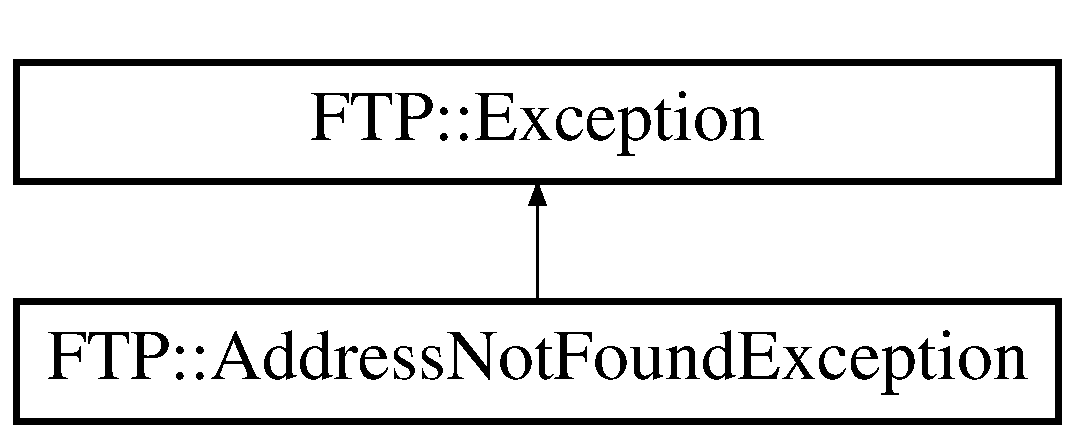
\includegraphics[height=2.000000cm]{classFTP_1_1AddressNotFoundException}
\end{center}
\end{figure}
\subsection*{Public Member Functions}
\begin{DoxyCompactItemize}
\item 
\hyperlink{classFTP_1_1AddressNotFoundException_a0a1d6bf81c4f0a1b1de50d253a187724}{Address\+Not\+Found\+Exception} (const std\+::string \&address)
\begin{DoxyCompactList}\small\item\em \hyperlink{classFTP_1_1AddressNotFoundException}{Address\+Not\+Found\+Exception} constructor. \end{DoxyCompactList}\end{DoxyCompactItemize}


\subsection{Detailed Description}
\hyperlink{classFTP_1_1Exception}{Exception} for Operating system error. 

\subsection{Constructor \& Destructor Documentation}
\hypertarget{classFTP_1_1AddressNotFoundException_a0a1d6bf81c4f0a1b1de50d253a187724}{}\index{F\+T\+P\+::\+Address\+Not\+Found\+Exception@{F\+T\+P\+::\+Address\+Not\+Found\+Exception}!Address\+Not\+Found\+Exception@{Address\+Not\+Found\+Exception}}
\index{Address\+Not\+Found\+Exception@{Address\+Not\+Found\+Exception}!F\+T\+P\+::\+Address\+Not\+Found\+Exception@{F\+T\+P\+::\+Address\+Not\+Found\+Exception}}
\subsubsection[{Address\+Not\+Found\+Exception}]{\setlength{\rightskip}{0pt plus 5cm}F\+T\+P\+::\+Address\+Not\+Found\+Exception\+::\+Address\+Not\+Found\+Exception (
\begin{DoxyParamCaption}
\item[{const std\+::string \&}]{address}
\end{DoxyParamCaption}
)}\label{classFTP_1_1AddressNotFoundException_a0a1d6bf81c4f0a1b1de50d253a187724}


\hyperlink{classFTP_1_1AddressNotFoundException}{Address\+Not\+Found\+Exception} constructor. 


\begin{DoxyParams}{Parameters}
{\em address} & The address which is not found \\
\hline
\end{DoxyParams}


The documentation for this class was generated from the following file\+:\begin{DoxyCompactItemize}
\item 
C\+:/\+Users/\+Nicolas Cachera/\+Documents/\+Programmation/\+C\+A\+R\+\_\+\+Furet\+T\+P/include/exception/Address\+Not\+Found\+Exception.\+h\end{DoxyCompactItemize}

\hypertarget{classFTP_1_1Answer}{}\section{F\+T\+P\+:\+:Answer Class Reference}
\label{classFTP_1_1Answer}\index{F\+T\+P\+::\+Answer@{F\+T\+P\+::\+Answer}}


Basic request\textquotesingle{}s answer.  




{\ttfamily \#include $<$Answer.\+h$>$}

Inheritance diagram for F\+T\+P\+:\+:Answer\+:\begin{figure}[H]
\begin{center}
\leavevmode
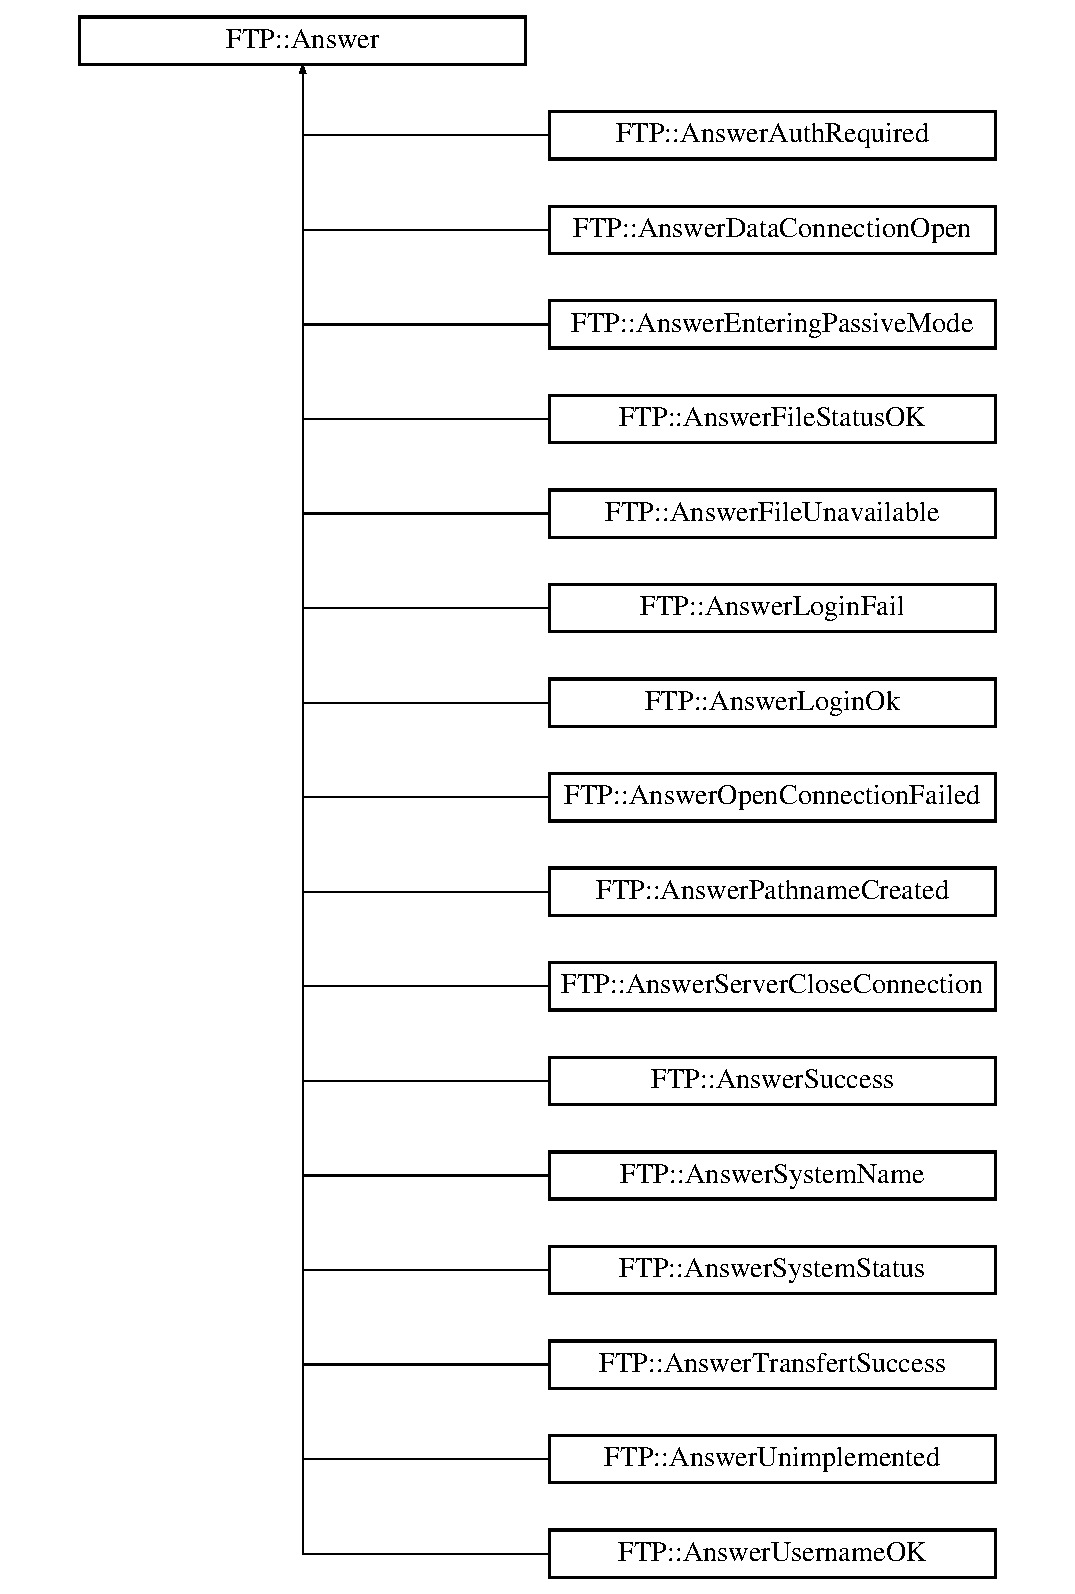
\includegraphics[height=12.000000cm]{classFTP_1_1Answer}
\end{center}
\end{figure}
\subsection*{Public Member Functions}
\begin{DoxyCompactItemize}
\item 
\hyperlink{classFTP_1_1Answer_a39151234c908f7e3028ee74d6290e8bf}{Answer} (unsigned int code)
\begin{DoxyCompactList}\small\item\em \hyperlink{classFTP_1_1Answer}{Answer} constructor. \end{DoxyCompactList}\item 
\hypertarget{classFTP_1_1Answer_abbba9b114d548fab7419060548b5f1e8}{}virtual \hyperlink{classFTP_1_1Answer_abbba9b114d548fab7419060548b5f1e8}{$\sim$\+Answer} ()\label{classFTP_1_1Answer_abbba9b114d548fab7419060548b5f1e8}

\begin{DoxyCompactList}\small\item\em \hyperlink{classFTP_1_1Answer}{Answer} desctructor. \end{DoxyCompactList}\item 
void \hyperlink{classFTP_1_1Answer_ac7d2718a9c3b31b620403d34dad8b55e}{generate\+Packet} (\hyperlink{classFTP_1_1Packet}{Packet} \&packet)
\begin{DoxyCompactList}\small\item\em generate\+Packet generate a packet to send to the user from the answer class. \end{DoxyCompactList}\item 
void \hyperlink{classFTP_1_1Answer_acd97d40fea4bb26e0e18429000d9705f}{add\+Argument} (const std\+::string \&argument)
\begin{DoxyCompactList}\small\item\em Add a string argument to the answer. \end{DoxyCompactList}\end{DoxyCompactItemize}


\subsection{Detailed Description}
Basic request\textquotesingle{}s answer. 

Represents a packet send by the server to the user in response of a request. 

\subsection{Constructor \& Destructor Documentation}
\hypertarget{classFTP_1_1Answer_a39151234c908f7e3028ee74d6290e8bf}{}\index{F\+T\+P\+::\+Answer@{F\+T\+P\+::\+Answer}!Answer@{Answer}}
\index{Answer@{Answer}!F\+T\+P\+::\+Answer@{F\+T\+P\+::\+Answer}}
\subsubsection[{Answer}]{\setlength{\rightskip}{0pt plus 5cm}F\+T\+P\+::\+Answer\+::\+Answer (
\begin{DoxyParamCaption}
\item[{unsigned int}]{code}
\end{DoxyParamCaption}
)}\label{classFTP_1_1Answer_a39151234c908f7e3028ee74d6290e8bf}


\hyperlink{classFTP_1_1Answer}{Answer} constructor. 


\begin{DoxyParams}{Parameters}
{\em code} & Return code value of the answer \\
\hline
\end{DoxyParams}


\subsection{Member Function Documentation}
\hypertarget{classFTP_1_1Answer_acd97d40fea4bb26e0e18429000d9705f}{}\index{F\+T\+P\+::\+Answer@{F\+T\+P\+::\+Answer}!add\+Argument@{add\+Argument}}
\index{add\+Argument@{add\+Argument}!F\+T\+P\+::\+Answer@{F\+T\+P\+::\+Answer}}
\subsubsection[{add\+Argument}]{\setlength{\rightskip}{0pt plus 5cm}void F\+T\+P\+::\+Answer\+::add\+Argument (
\begin{DoxyParamCaption}
\item[{const std\+::string \&}]{argument}
\end{DoxyParamCaption}
)}\label{classFTP_1_1Answer_acd97d40fea4bb26e0e18429000d9705f}


Add a string argument to the answer. 


\begin{DoxyParams}{Parameters}
{\em argument} & the string to add \\
\hline
\end{DoxyParams}
\hypertarget{classFTP_1_1Answer_ac7d2718a9c3b31b620403d34dad8b55e}{}\index{F\+T\+P\+::\+Answer@{F\+T\+P\+::\+Answer}!generate\+Packet@{generate\+Packet}}
\index{generate\+Packet@{generate\+Packet}!F\+T\+P\+::\+Answer@{F\+T\+P\+::\+Answer}}
\subsubsection[{generate\+Packet}]{\setlength{\rightskip}{0pt plus 5cm}void F\+T\+P\+::\+Answer\+::generate\+Packet (
\begin{DoxyParamCaption}
\item[{{\bf Packet} \&}]{packet}
\end{DoxyParamCaption}
)}\label{classFTP_1_1Answer_ac7d2718a9c3b31b620403d34dad8b55e}


generate\+Packet generate a packet to send to the user from the answer class. 


\begin{DoxyParams}{Parameters}
{\em packet} & \hyperlink{classFTP_1_1Packet}{Packet} which will contains the generated packet\\
\hline
\end{DoxyParams}
The packet will have the following format \+: $<$\+\_\+code$>$ $<$\+\_\+arguments$>$. 

The documentation for this class was generated from the following file\+:\begin{DoxyCompactItemize}
\item 
C\+:/\+Users/\+Nicolas Cachera/\+Documents/\+Programmation/\+C\+A\+R\+\_\+\+Furet\+T\+P/include/core/message/answer/Answer.\+h\end{DoxyCompactItemize}

\hypertarget{classFTP_1_1AnswerAuthRequired}{}\section{F\+T\+P\+:\+:Answer\+Auth\+Required Class Reference}
\label{classFTP_1_1AnswerAuthRequired}\index{F\+T\+P\+::\+Answer\+Auth\+Required@{F\+T\+P\+::\+Answer\+Auth\+Required}}


532 need account for storing files.  




{\ttfamily \#include $<$Answer\+Command\+Error.\+h$>$}

Inheritance diagram for F\+T\+P\+:\+:Answer\+Auth\+Required\+:\begin{figure}[H]
\begin{center}
\leavevmode
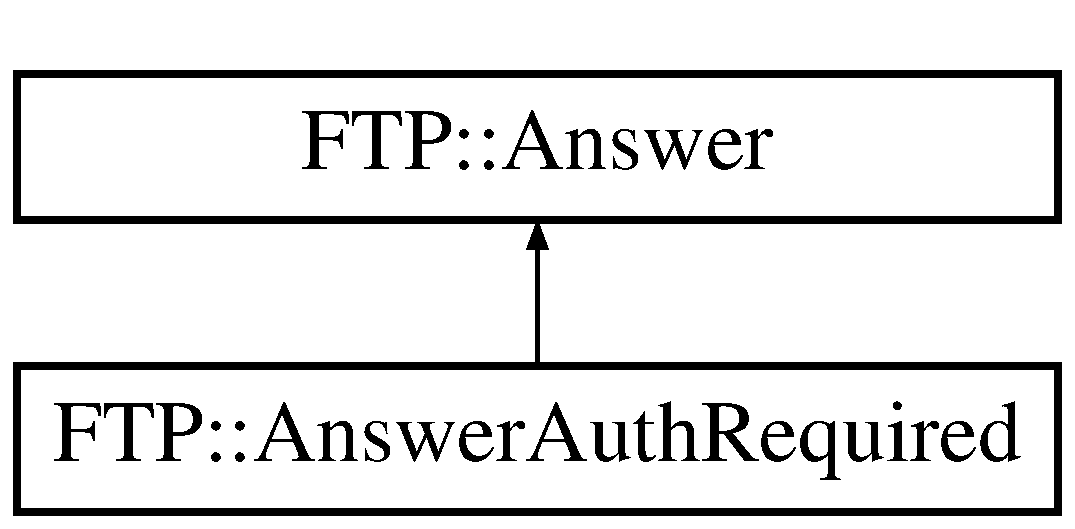
\includegraphics[height=2.000000cm]{classFTP_1_1AnswerAuthRequired}
\end{center}
\end{figure}
\subsection*{Static Public Attributes}
\begin{DoxyCompactItemize}
\item 
\hypertarget{classFTP_1_1AnswerAuthRequired_a0b31d375012cdc068704bcf4d1a88bf3}{}static const unsigned int {\bfseries Code} = 532\label{classFTP_1_1AnswerAuthRequired_a0b31d375012cdc068704bcf4d1a88bf3}

\end{DoxyCompactItemize}
\subsection*{Additional Inherited Members}


\subsection{Detailed Description}
532 need account for storing files. 

The documentation for this class was generated from the following file\+:\begin{DoxyCompactItemize}
\item 
C\+:/\+Users/\+Nicolas Cachera/\+Documents/\+Programmation/\+C\+A\+R\+\_\+\+Furet\+T\+P/include/core/message/answer/Answer\+Command\+Error.\+h\end{DoxyCompactItemize}

\hypertarget{classFTP_1_1AnswerDataConnectionOpen}{}\section{F\+T\+P\+:\+:Answer\+Data\+Connection\+Open Class Reference}
\label{classFTP_1_1AnswerDataConnectionOpen}\index{F\+T\+P\+::\+Answer\+Data\+Connection\+Open@{F\+T\+P\+::\+Answer\+Data\+Connection\+Open}}


225 Data connection open, no transfert in progress  




{\ttfamily \#include $<$Answer\+Success.\+h$>$}

Inheritance diagram for F\+T\+P\+:\+:Answer\+Data\+Connection\+Open\+:\begin{figure}[H]
\begin{center}
\leavevmode
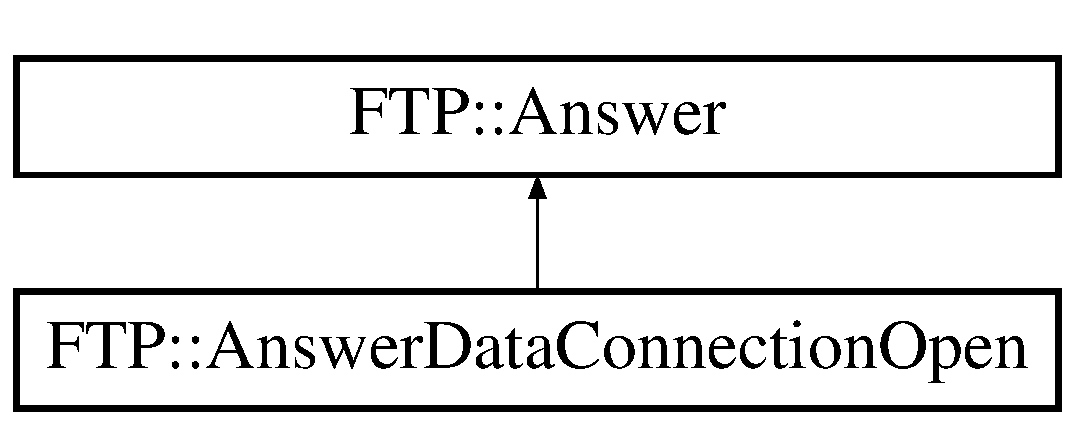
\includegraphics[height=2.000000cm]{classFTP_1_1AnswerDataConnectionOpen}
\end{center}
\end{figure}
\subsection*{Static Public Attributes}
\begin{DoxyCompactItemize}
\item 
\hypertarget{classFTP_1_1AnswerDataConnectionOpen_a883697754f0cebfe3f8f6be47f6461c0}{}static const unsigned int {\bfseries Code} = 225\label{classFTP_1_1AnswerDataConnectionOpen_a883697754f0cebfe3f8f6be47f6461c0}

\end{DoxyCompactItemize}
\subsection*{Additional Inherited Members}


\subsection{Detailed Description}
225 Data connection open, no transfert in progress 

The documentation for this class was generated from the following file\+:\begin{DoxyCompactItemize}
\item 
C\+:/\+Users/\+Nicolas Cachera/\+Documents/\+Programmation/\+C\+A\+R\+\_\+\+Furet\+T\+P/include/core/message/answer/Answer\+Success.\+h\end{DoxyCompactItemize}

\hypertarget{classFTP_1_1AnswerEnteringPassiveMode}{}\section{F\+T\+P\+:\+:Answer\+Entering\+Passive\+Mode Class Reference}
\label{classFTP_1_1AnswerEnteringPassiveMode}\index{F\+T\+P\+::\+Answer\+Entering\+Passive\+Mode@{F\+T\+P\+::\+Answer\+Entering\+Passive\+Mode}}


227 Entering passive mode  




{\ttfamily \#include $<$Answer\+Success.\+h$>$}

Inheritance diagram for F\+T\+P\+:\+:Answer\+Entering\+Passive\+Mode\+:\begin{figure}[H]
\begin{center}
\leavevmode
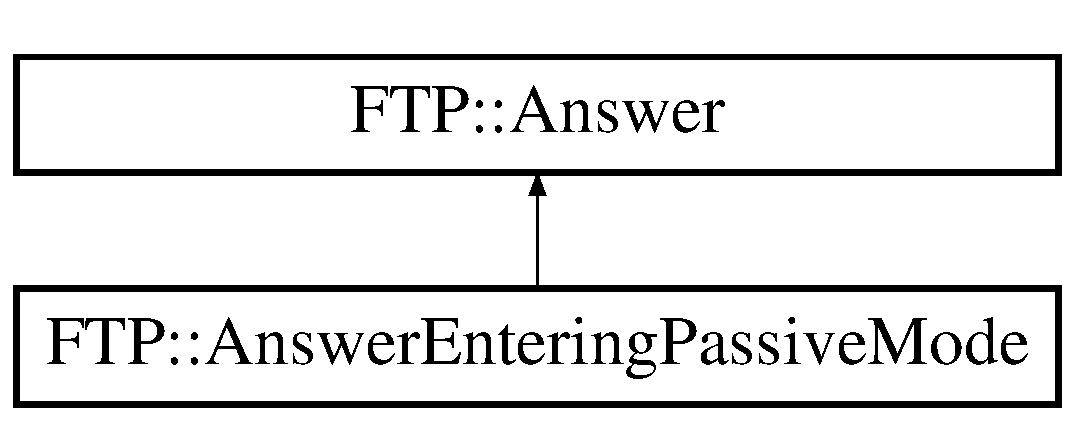
\includegraphics[height=2.000000cm]{classFTP_1_1AnswerEnteringPassiveMode}
\end{center}
\end{figure}
\subsection*{Static Public Attributes}
\begin{DoxyCompactItemize}
\item 
\hypertarget{classFTP_1_1AnswerEnteringPassiveMode_a3f6261b4cfda714e0611d9184e698c6d}{}static const unsigned int {\bfseries Code} = 227\label{classFTP_1_1AnswerEnteringPassiveMode_a3f6261b4cfda714e0611d9184e698c6d}

\end{DoxyCompactItemize}
\subsection*{Additional Inherited Members}


\subsection{Detailed Description}
227 Entering passive mode 

The documentation for this class was generated from the following file\+:\begin{DoxyCompactItemize}
\item 
C\+:/\+Users/\+Nicolas Cachera/\+Documents/\+Programmation/\+C\+A\+R\+\_\+\+Furet\+T\+P/include/core/message/answer/Answer\+Success.\+h\end{DoxyCompactItemize}

\hypertarget{classFTP_1_1AnswerFileStatusOK}{}\section{F\+T\+P\+:\+:Answer\+File\+Status\+O\+K Class Reference}
\label{classFTP_1_1AnswerFileStatusOK}\index{F\+T\+P\+::\+Answer\+File\+Status\+O\+K@{F\+T\+P\+::\+Answer\+File\+Status\+O\+K}}


150 file status okay; about to open data connection.  




{\ttfamily \#include $<$Answer\+Initialize.\+h$>$}

Inheritance diagram for F\+T\+P\+:\+:Answer\+File\+Status\+O\+K\+:\begin{figure}[H]
\begin{center}
\leavevmode
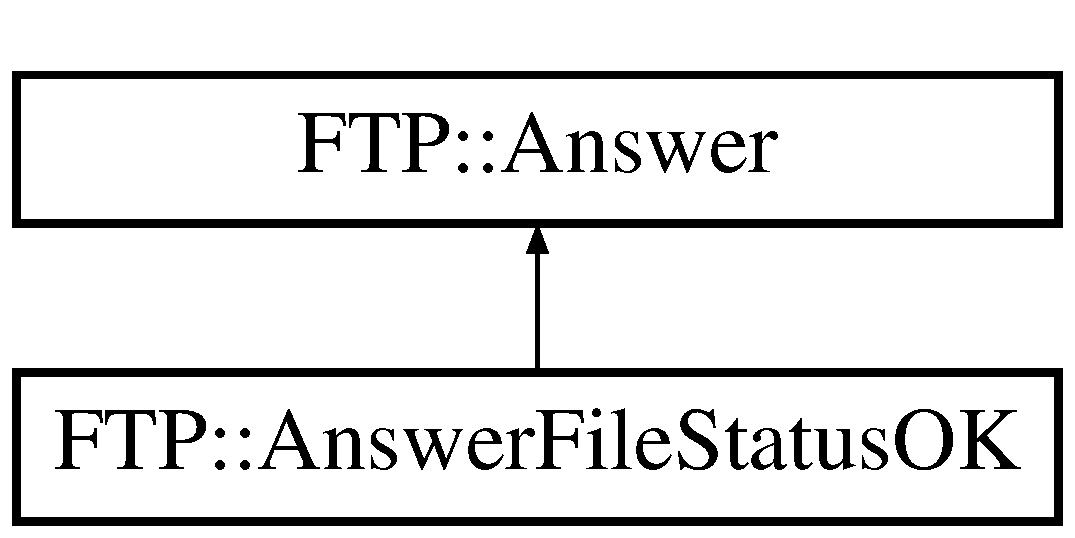
\includegraphics[height=2.000000cm]{classFTP_1_1AnswerFileStatusOK}
\end{center}
\end{figure}
\subsection*{Static Public Attributes}
\begin{DoxyCompactItemize}
\item 
\hypertarget{classFTP_1_1AnswerFileStatusOK_abbcdece8e9af326b425d4d0ec456835b}{}static const unsigned int {\bfseries Code} = 150\label{classFTP_1_1AnswerFileStatusOK_abbcdece8e9af326b425d4d0ec456835b}

\end{DoxyCompactItemize}
\subsection*{Additional Inherited Members}


\subsection{Detailed Description}
150 file status okay; about to open data connection. 

The documentation for this class was generated from the following file\+:\begin{DoxyCompactItemize}
\item 
C\+:/\+Users/\+Nicolas Cachera/\+Documents/\+Programmation/\+C\+A\+R\+\_\+\+Furet\+T\+P/include/core/message/answer/Answer\+Initialize.\+h\end{DoxyCompactItemize}

\hypertarget{classFTP_1_1AnswerFileUnavailable}{}\section{F\+T\+P\+:\+:Answer\+File\+Unavailable Class Reference}
\label{classFTP_1_1AnswerFileUnavailable}\index{F\+T\+P\+::\+Answer\+File\+Unavailable@{F\+T\+P\+::\+Answer\+File\+Unavailable}}


550 file unavailable  




{\ttfamily \#include $<$Answer\+Command\+Error.\+h$>$}

Inheritance diagram for F\+T\+P\+:\+:Answer\+File\+Unavailable\+:\begin{figure}[H]
\begin{center}
\leavevmode
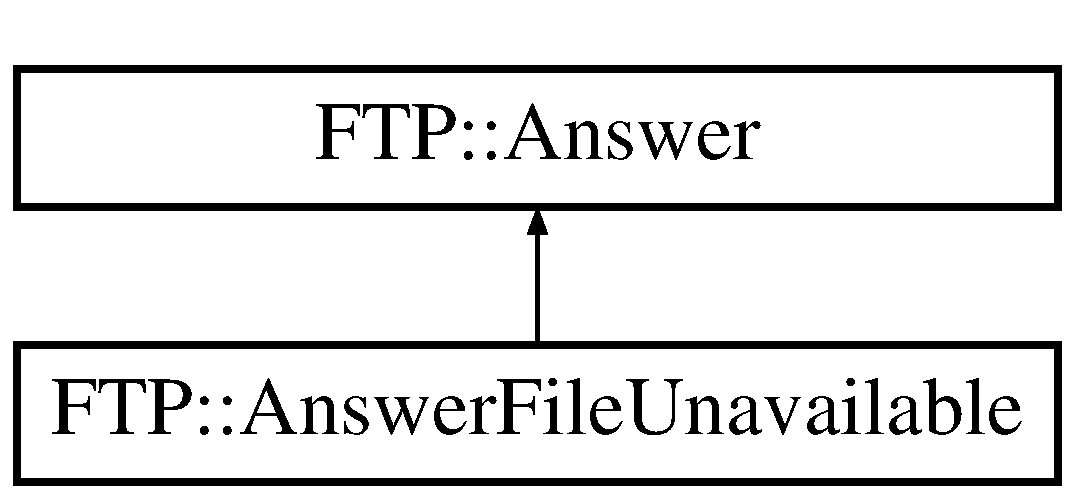
\includegraphics[height=2.000000cm]{classFTP_1_1AnswerFileUnavailable}
\end{center}
\end{figure}
\subsection*{Static Public Attributes}
\begin{DoxyCompactItemize}
\item 
\hypertarget{classFTP_1_1AnswerFileUnavailable_adf574d290aa6e1609cce557f7d54515f}{}static const unsigned int {\bfseries Code} = 550\label{classFTP_1_1AnswerFileUnavailable_adf574d290aa6e1609cce557f7d54515f}

\end{DoxyCompactItemize}
\subsection*{Additional Inherited Members}


\subsection{Detailed Description}
550 file unavailable 

The documentation for this class was generated from the following file\+:\begin{DoxyCompactItemize}
\item 
C\+:/\+Users/\+Nicolas Cachera/\+Documents/\+Programmation/\+C\+A\+R\+\_\+\+Furet\+T\+P/include/core/message/answer/Answer\+Command\+Error.\+h\end{DoxyCompactItemize}

\hypertarget{classFTP_1_1AnswerLoginFail}{}\section{F\+T\+P\+:\+:Answer\+Login\+Fail Class Reference}
\label{classFTP_1_1AnswerLoginFail}\index{F\+T\+P\+::\+Answer\+Login\+Fail@{F\+T\+P\+::\+Answer\+Login\+Fail}}


430 Username or password incorrect  




{\ttfamily \#include $<$Answer\+User\+Error.\+h$>$}

Inheritance diagram for F\+T\+P\+:\+:Answer\+Login\+Fail\+:\begin{figure}[H]
\begin{center}
\leavevmode
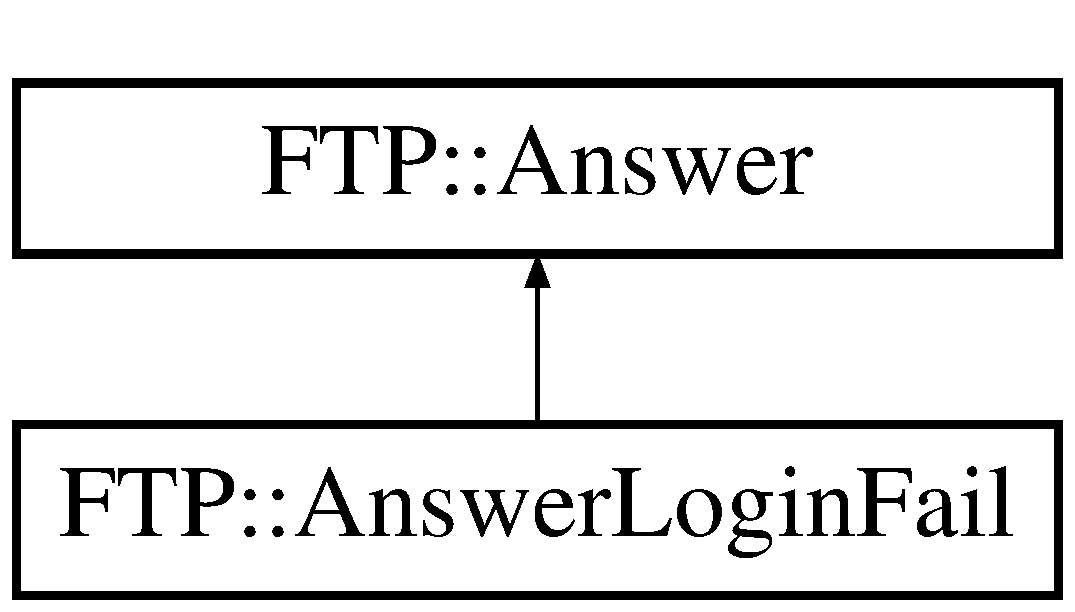
\includegraphics[height=2.000000cm]{classFTP_1_1AnswerLoginFail}
\end{center}
\end{figure}
\subsection*{Static Public Attributes}
\begin{DoxyCompactItemize}
\item 
\hypertarget{classFTP_1_1AnswerLoginFail_add2a45cb80065adb45244ffd47b10ce5}{}static const unsigned int {\bfseries Code} = 430\label{classFTP_1_1AnswerLoginFail_add2a45cb80065adb45244ffd47b10ce5}

\end{DoxyCompactItemize}
\subsection*{Additional Inherited Members}


\subsection{Detailed Description}
430 Username or password incorrect 

The documentation for this class was generated from the following file\+:\begin{DoxyCompactItemize}
\item 
C\+:/\+Users/\+Nicolas Cachera/\+Documents/\+Programmation/\+C\+A\+R\+\_\+\+Furet\+T\+P/include/core/message/answer/Answer\+User\+Error.\+h\end{DoxyCompactItemize}

\hypertarget{classFTP_1_1AnswerLoginOk}{}\section{F\+T\+P\+:\+:Answer\+Login\+Ok Class Reference}
\label{classFTP_1_1AnswerLoginOk}\index{F\+T\+P\+::\+Answer\+Login\+Ok@{F\+T\+P\+::\+Answer\+Login\+Ok}}


230 \hyperlink{structFTP_1_1User}{User} identifiant ok  




{\ttfamily \#include $<$Answer\+Success.\+h$>$}

Inheritance diagram for F\+T\+P\+:\+:Answer\+Login\+Ok\+:\begin{figure}[H]
\begin{center}
\leavevmode
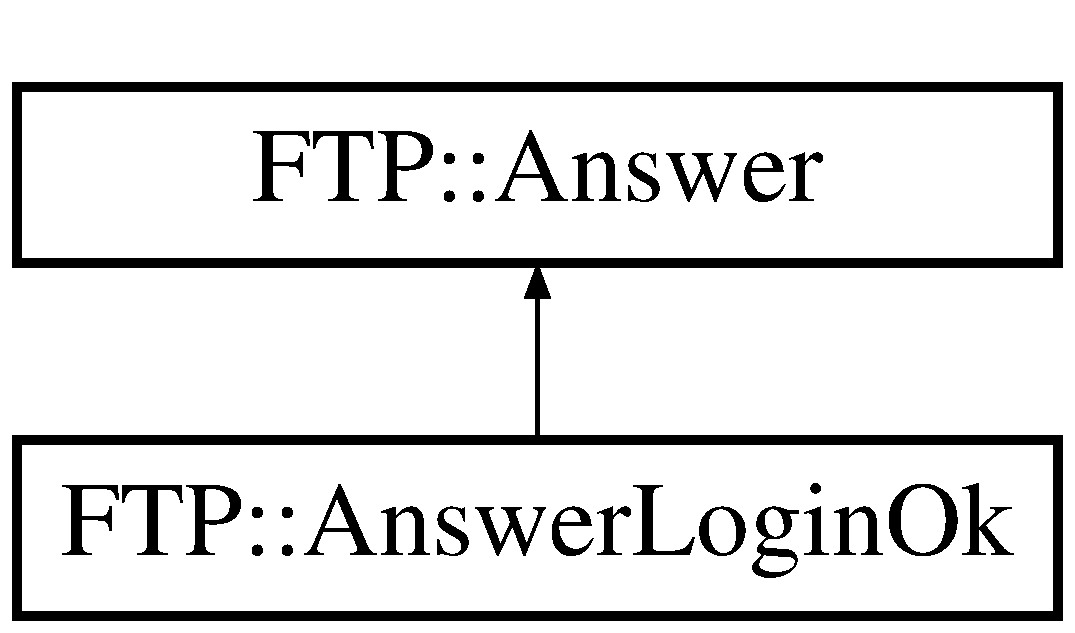
\includegraphics[height=2.000000cm]{classFTP_1_1AnswerLoginOk}
\end{center}
\end{figure}
\subsection*{Static Public Attributes}
\begin{DoxyCompactItemize}
\item 
\hypertarget{classFTP_1_1AnswerLoginOk_a5931c280d254e2cddbab352d225f2398}{}static const unsigned int {\bfseries Code} = 230\label{classFTP_1_1AnswerLoginOk_a5931c280d254e2cddbab352d225f2398}

\end{DoxyCompactItemize}
\subsection*{Additional Inherited Members}


\subsection{Detailed Description}
230 \hyperlink{structFTP_1_1User}{User} identifiant ok 

The documentation for this class was generated from the following file\+:\begin{DoxyCompactItemize}
\item 
C\+:/\+Users/\+Nicolas Cachera/\+Documents/\+Programmation/\+C\+A\+R\+\_\+\+Furet\+T\+P/include/core/message/answer/Answer\+Success.\+h\end{DoxyCompactItemize}

\hypertarget{classFTP_1_1AnswerOpenConnectionFailed}{}\section{F\+T\+P\+:\+:Answer\+Open\+Connection\+Failed Class Reference}
\label{classFTP_1_1AnswerOpenConnectionFailed}\index{F\+T\+P\+::\+Answer\+Open\+Connection\+Failed@{F\+T\+P\+::\+Answer\+Open\+Connection\+Failed}}


425 Can\textquotesingle{}t open a data connection  




{\ttfamily \#include $<$Answer\+User\+Error.\+h$>$}

Inheritance diagram for F\+T\+P\+:\+:Answer\+Open\+Connection\+Failed\+:\begin{figure}[H]
\begin{center}
\leavevmode
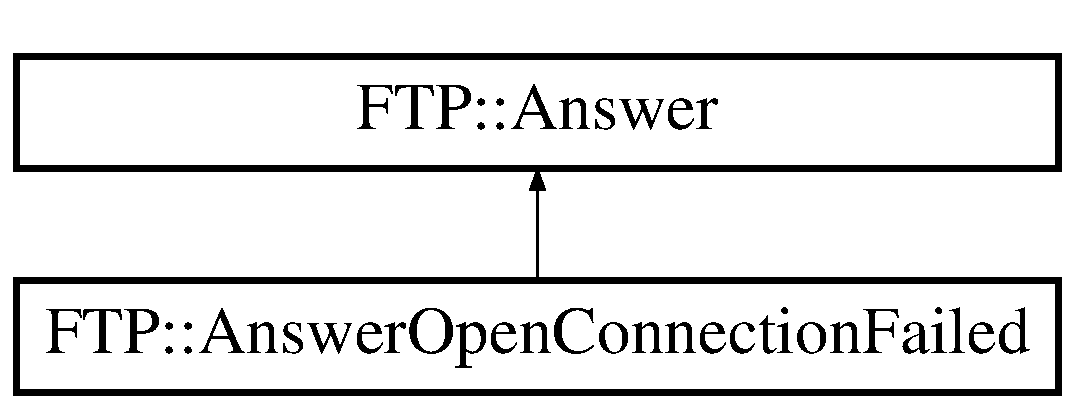
\includegraphics[height=2.000000cm]{classFTP_1_1AnswerOpenConnectionFailed}
\end{center}
\end{figure}
\subsection*{Static Public Attributes}
\begin{DoxyCompactItemize}
\item 
\hypertarget{classFTP_1_1AnswerOpenConnectionFailed_ab58e3bd133a6b97fcf460bd0ea4550d7}{}static const unsigned int {\bfseries Code} = 425\label{classFTP_1_1AnswerOpenConnectionFailed_ab58e3bd133a6b97fcf460bd0ea4550d7}

\end{DoxyCompactItemize}
\subsection*{Additional Inherited Members}


\subsection{Detailed Description}
425 Can\textquotesingle{}t open a data connection 

The documentation for this class was generated from the following file\+:\begin{DoxyCompactItemize}
\item 
C\+:/\+Users/\+Nicolas Cachera/\+Documents/\+Programmation/\+C\+A\+R\+\_\+\+Furet\+T\+P/include/core/message/answer/Answer\+User\+Error.\+h\end{DoxyCompactItemize}

\hypertarget{classFTP_1_1AnswerPathnameCreated}{}\section{F\+T\+P\+:\+:Answer\+Pathname\+Created Class Reference}
\label{classFTP_1_1AnswerPathnameCreated}\index{F\+T\+P\+::\+Answer\+Pathname\+Created@{F\+T\+P\+::\+Answer\+Pathname\+Created}}


257 System pathname  




{\ttfamily \#include $<$Answer\+Success.\+h$>$}

Inheritance diagram for F\+T\+P\+:\+:Answer\+Pathname\+Created\+:\begin{figure}[H]
\begin{center}
\leavevmode
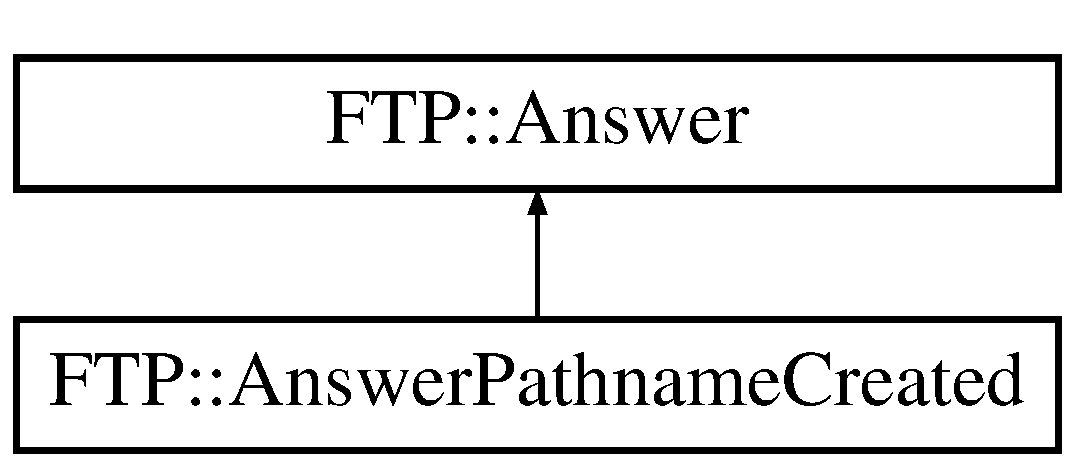
\includegraphics[height=2.000000cm]{classFTP_1_1AnswerPathnameCreated}
\end{center}
\end{figure}
\subsection*{Static Public Attributes}
\begin{DoxyCompactItemize}
\item 
\hypertarget{classFTP_1_1AnswerPathnameCreated_a318289d8af475a7ff1b55b0a7cddc503}{}static const unsigned int {\bfseries Code} = 257\label{classFTP_1_1AnswerPathnameCreated_a318289d8af475a7ff1b55b0a7cddc503}

\end{DoxyCompactItemize}
\subsection*{Additional Inherited Members}


\subsection{Detailed Description}
257 System pathname 

The documentation for this class was generated from the following file\+:\begin{DoxyCompactItemize}
\item 
C\+:/\+Users/\+Nicolas Cachera/\+Documents/\+Programmation/\+C\+A\+R\+\_\+\+Furet\+T\+P/include/core/message/answer/Answer\+Success.\+h\end{DoxyCompactItemize}

\hypertarget{classFTP_1_1AnswerServerCloseConnection}{}\section{F\+T\+P\+:\+:Answer\+Server\+Close\+Connection Class Reference}
\label{classFTP_1_1AnswerServerCloseConnection}\index{F\+T\+P\+::\+Answer\+Server\+Close\+Connection@{F\+T\+P\+::\+Answer\+Server\+Close\+Connection}}


221 server close connection  




{\ttfamily \#include $<$Answer\+Success.\+h$>$}

Inheritance diagram for F\+T\+P\+:\+:Answer\+Server\+Close\+Connection\+:\begin{figure}[H]
\begin{center}
\leavevmode
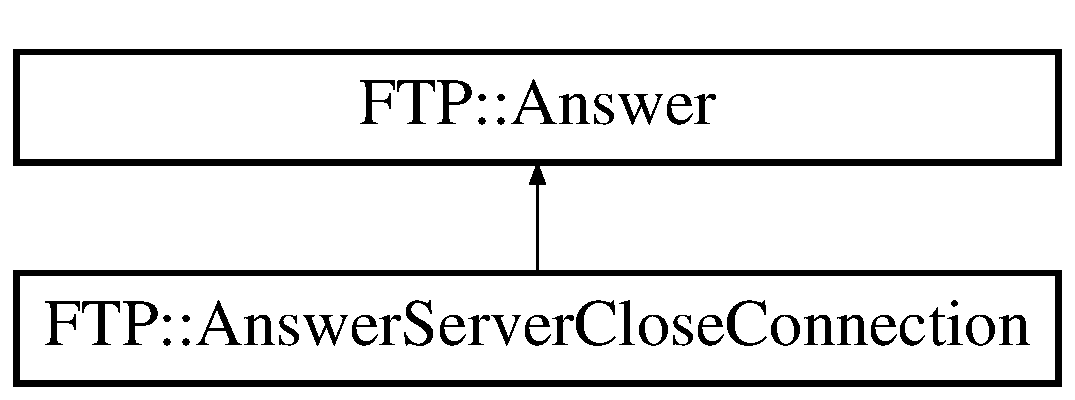
\includegraphics[height=2.000000cm]{classFTP_1_1AnswerServerCloseConnection}
\end{center}
\end{figure}
\subsection*{Static Public Attributes}
\begin{DoxyCompactItemize}
\item 
\hypertarget{classFTP_1_1AnswerServerCloseConnection_a84a59678802f8cb1a193b407e05b6814}{}static const unsigned int {\bfseries Code} = 221\label{classFTP_1_1AnswerServerCloseConnection_a84a59678802f8cb1a193b407e05b6814}

\end{DoxyCompactItemize}
\subsection*{Additional Inherited Members}


\subsection{Detailed Description}
221 server close connection 

The documentation for this class was generated from the following file\+:\begin{DoxyCompactItemize}
\item 
C\+:/\+Users/\+Nicolas Cachera/\+Documents/\+Programmation/\+C\+A\+R\+\_\+\+Furet\+T\+P/include/core/message/answer/Answer\+Success.\+h\end{DoxyCompactItemize}

\hypertarget{classFTP_1_1AnswerSuccess}{}\section{F\+T\+P\+:\+:Answer\+Success Class Reference}
\label{classFTP_1_1AnswerSuccess}\index{F\+T\+P\+::\+Answer\+Success@{F\+T\+P\+::\+Answer\+Success}}


200 O\+K  




{\ttfamily \#include $<$Answer\+Success.\+h$>$}

Inheritance diagram for F\+T\+P\+:\+:Answer\+Success\+:\begin{figure}[H]
\begin{center}
\leavevmode
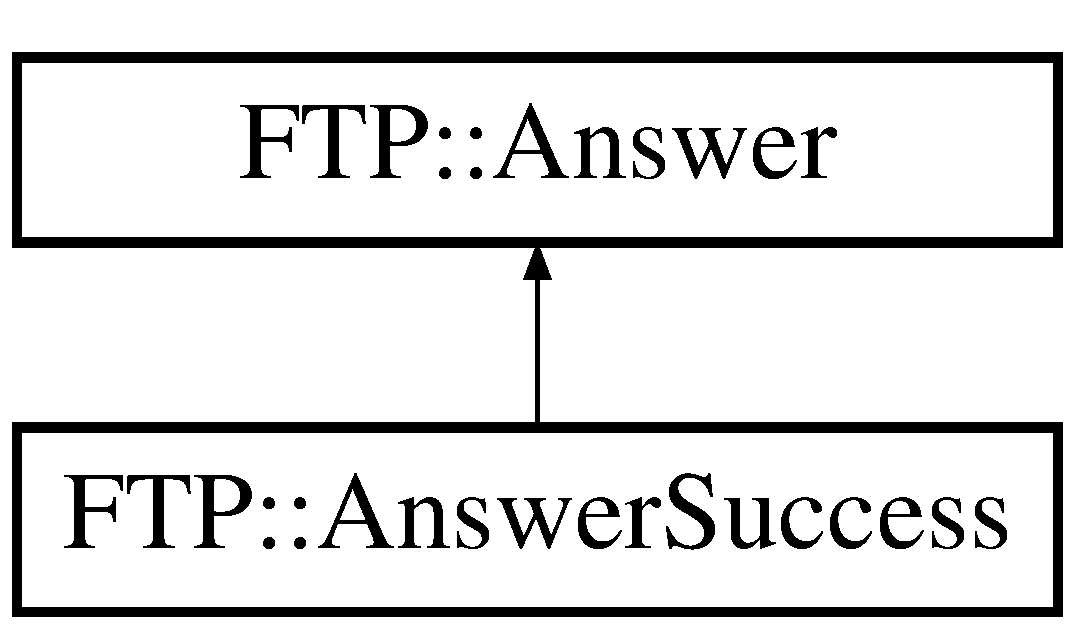
\includegraphics[height=2.000000cm]{classFTP_1_1AnswerSuccess}
\end{center}
\end{figure}
\subsection*{Static Public Attributes}
\begin{DoxyCompactItemize}
\item 
\hypertarget{classFTP_1_1AnswerSuccess_a3708e95f733d7e0d8aa62864113dc20b}{}static const unsigned int {\bfseries Code} = 200\label{classFTP_1_1AnswerSuccess_a3708e95f733d7e0d8aa62864113dc20b}

\end{DoxyCompactItemize}
\subsection*{Additional Inherited Members}


\subsection{Detailed Description}
200 O\+K 

The documentation for this class was generated from the following file\+:\begin{DoxyCompactItemize}
\item 
C\+:/\+Users/\+Nicolas Cachera/\+Documents/\+Programmation/\+C\+A\+R\+\_\+\+Furet\+T\+P/include/core/message/answer/Answer\+Success.\+h\end{DoxyCompactItemize}

\hypertarget{classFTP_1_1AnswerSystemName}{}\section{F\+T\+P\+:\+:Answer\+System\+Name Class Reference}
\label{classFTP_1_1AnswerSystemName}\index{F\+T\+P\+::\+Answer\+System\+Name@{F\+T\+P\+::\+Answer\+System\+Name}}


215 System name  




{\ttfamily \#include $<$Answer\+Success.\+h$>$}

Inheritance diagram for F\+T\+P\+:\+:Answer\+System\+Name\+:\begin{figure}[H]
\begin{center}
\leavevmode
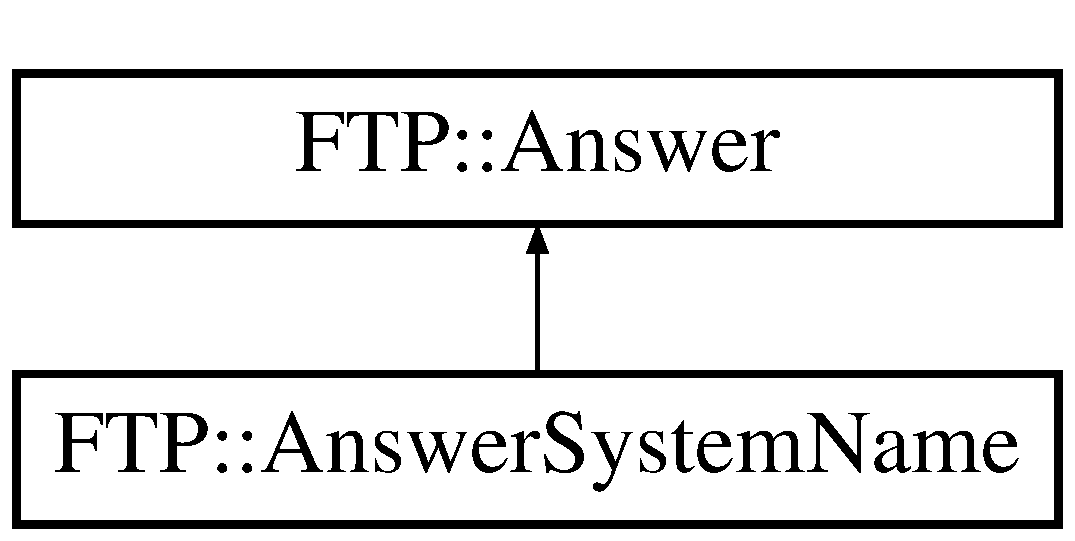
\includegraphics[height=2.000000cm]{classFTP_1_1AnswerSystemName}
\end{center}
\end{figure}
\subsection*{Public Member Functions}
\begin{DoxyCompactItemize}
\item 
\hypertarget{classFTP_1_1AnswerSystemName_a435757c81d82db47f1935c241c906023}{}{\bfseries Answer\+System\+Name} (const std\+::string \&system\+Name)\label{classFTP_1_1AnswerSystemName_a435757c81d82db47f1935c241c906023}

\end{DoxyCompactItemize}
\subsection*{Static Public Attributes}
\begin{DoxyCompactItemize}
\item 
\hypertarget{classFTP_1_1AnswerSystemName_af8ce22730f7209c5c72d3827fe6eb3b3}{}static const unsigned int {\bfseries Code} = 215\label{classFTP_1_1AnswerSystemName_af8ce22730f7209c5c72d3827fe6eb3b3}

\end{DoxyCompactItemize}


\subsection{Detailed Description}
215 System name 

The documentation for this class was generated from the following file\+:\begin{DoxyCompactItemize}
\item 
C\+:/\+Users/\+Nicolas Cachera/\+Documents/\+Programmation/\+C\+A\+R\+\_\+\+Furet\+T\+P/include/core/message/answer/Answer\+Success.\+h\end{DoxyCompactItemize}

\hypertarget{classFTP_1_1AnswerSystemStatus}{}\section{F\+T\+P\+:\+:Answer\+System\+Status Class Reference}
\label{classFTP_1_1AnswerSystemStatus}\index{F\+T\+P\+::\+Answer\+System\+Status@{F\+T\+P\+::\+Answer\+System\+Status}}


211 System status  




{\ttfamily \#include $<$Answer\+Success.\+h$>$}

Inheritance diagram for F\+T\+P\+:\+:Answer\+System\+Status\+:\begin{figure}[H]
\begin{center}
\leavevmode
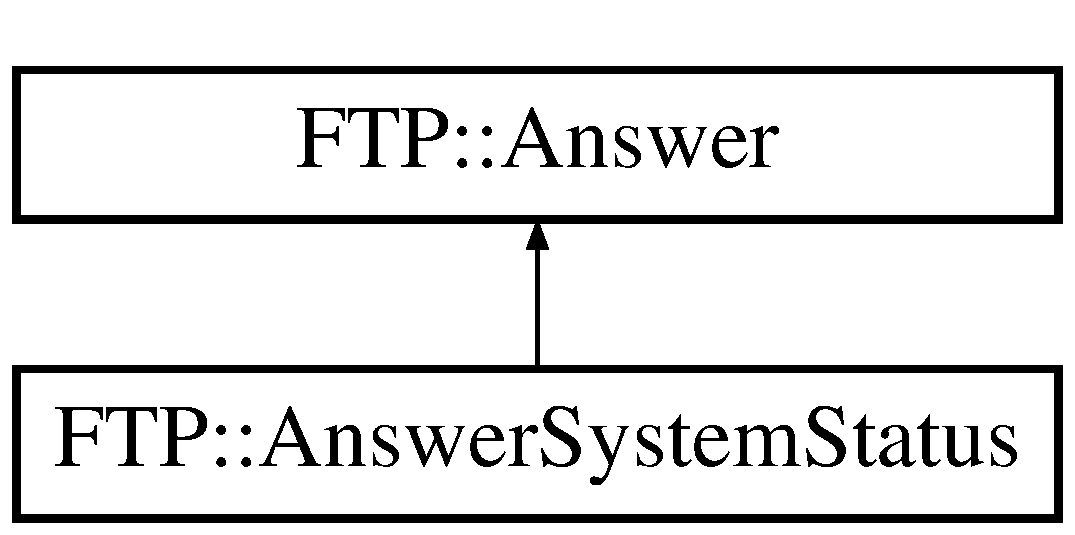
\includegraphics[height=2.000000cm]{classFTP_1_1AnswerSystemStatus}
\end{center}
\end{figure}
\subsection*{Static Public Attributes}
\begin{DoxyCompactItemize}
\item 
\hypertarget{classFTP_1_1AnswerSystemStatus_abb133d330c4bffaab044b3300ed49a65}{}static const unsigned int {\bfseries Code} = 211\label{classFTP_1_1AnswerSystemStatus_abb133d330c4bffaab044b3300ed49a65}

\end{DoxyCompactItemize}
\subsection*{Additional Inherited Members}


\subsection{Detailed Description}
211 System status 

The documentation for this class was generated from the following file\+:\begin{DoxyCompactItemize}
\item 
C\+:/\+Users/\+Nicolas Cachera/\+Documents/\+Programmation/\+C\+A\+R\+\_\+\+Furet\+T\+P/include/core/message/answer/Answer\+Success.\+h\end{DoxyCompactItemize}

\hypertarget{classFTP_1_1AnswerTransfertSuccess}{}\section{F\+T\+P\+:\+:Answer\+Transfert\+Success Class Reference}
\label{classFTP_1_1AnswerTransfertSuccess}\index{F\+T\+P\+::\+Answer\+Transfert\+Success@{F\+T\+P\+::\+Answer\+Transfert\+Success}}


226 File transfert success  




{\ttfamily \#include $<$Answer\+Success.\+h$>$}

Inheritance diagram for F\+T\+P\+:\+:Answer\+Transfert\+Success\+:\begin{figure}[H]
\begin{center}
\leavevmode
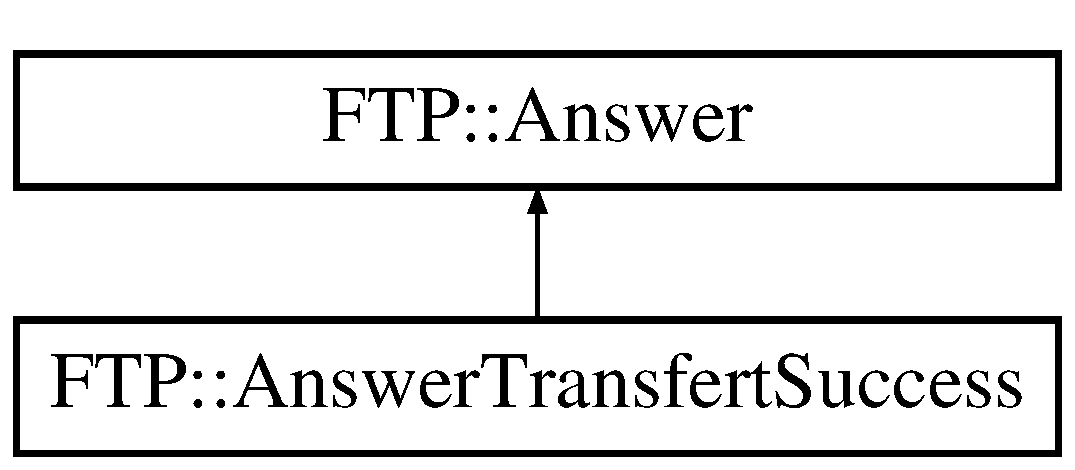
\includegraphics[height=2.000000cm]{classFTP_1_1AnswerTransfertSuccess}
\end{center}
\end{figure}
\subsection*{Static Public Attributes}
\begin{DoxyCompactItemize}
\item 
\hypertarget{classFTP_1_1AnswerTransfertSuccess_a5f298ee0643cb6879316cda93e94ea3f}{}static const unsigned int {\bfseries Code} = 226\label{classFTP_1_1AnswerTransfertSuccess_a5f298ee0643cb6879316cda93e94ea3f}

\end{DoxyCompactItemize}
\subsection*{Additional Inherited Members}


\subsection{Detailed Description}
226 File transfert success 

The documentation for this class was generated from the following file\+:\begin{DoxyCompactItemize}
\item 
C\+:/\+Users/\+Nicolas Cachera/\+Documents/\+Programmation/\+C\+A\+R\+\_\+\+Furet\+T\+P/include/core/message/answer/Answer\+Success.\+h\end{DoxyCompactItemize}

\hypertarget{classFTP_1_1AnswerUnimplemented}{}\section{F\+T\+P\+:\+:Answer\+Unimplemented Class Reference}
\label{classFTP_1_1AnswerUnimplemented}\index{F\+T\+P\+::\+Answer\+Unimplemented@{F\+T\+P\+::\+Answer\+Unimplemented}}


502 unimplemented command  




{\ttfamily \#include $<$Answer\+Command\+Error.\+h$>$}

Inheritance diagram for F\+T\+P\+:\+:Answer\+Unimplemented\+:\begin{figure}[H]
\begin{center}
\leavevmode
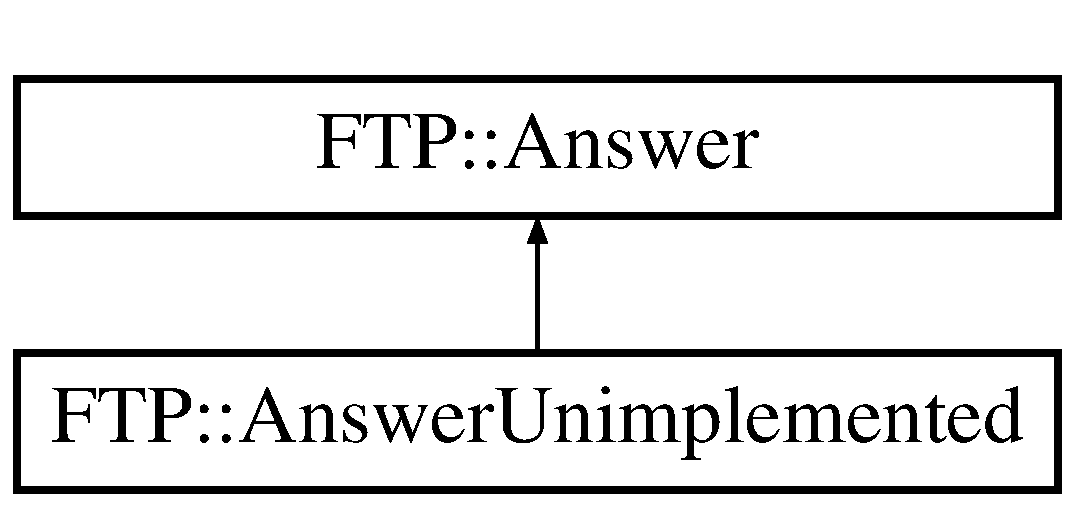
\includegraphics[height=2.000000cm]{classFTP_1_1AnswerUnimplemented}
\end{center}
\end{figure}
\subsection*{Static Public Attributes}
\begin{DoxyCompactItemize}
\item 
\hypertarget{classFTP_1_1AnswerUnimplemented_a2cd23d0c7ad3f6c5b353012a27cc1fcd}{}static const unsigned int {\bfseries Code} = 502\label{classFTP_1_1AnswerUnimplemented_a2cd23d0c7ad3f6c5b353012a27cc1fcd}

\end{DoxyCompactItemize}
\subsection*{Additional Inherited Members}


\subsection{Detailed Description}
502 unimplemented command 

The documentation for this class was generated from the following file\+:\begin{DoxyCompactItemize}
\item 
C\+:/\+Users/\+Nicolas Cachera/\+Documents/\+Programmation/\+C\+A\+R\+\_\+\+Furet\+T\+P/include/core/message/answer/Answer\+Command\+Error.\+h\end{DoxyCompactItemize}

\hypertarget{classFTP_1_1AnswerUsernameOK}{}\section{F\+T\+P\+:\+:Answer\+Username\+O\+K Class Reference}
\label{classFTP_1_1AnswerUsernameOK}\index{F\+T\+P\+::\+Answer\+Username\+O\+K@{F\+T\+P\+::\+Answer\+Username\+O\+K}}


331 Username O\+K, require password  




{\ttfamily \#include $<$Answer\+Waiting.\+h$>$}

Inheritance diagram for F\+T\+P\+:\+:Answer\+Username\+O\+K\+:\begin{figure}[H]
\begin{center}
\leavevmode
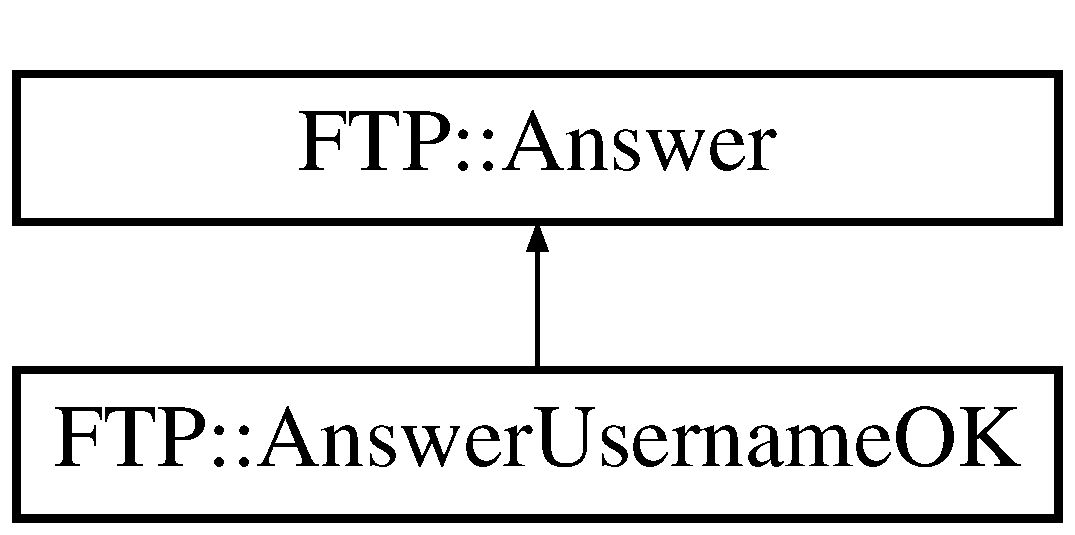
\includegraphics[height=2.000000cm]{classFTP_1_1AnswerUsernameOK}
\end{center}
\end{figure}
\subsection*{Static Public Attributes}
\begin{DoxyCompactItemize}
\item 
\hypertarget{classFTP_1_1AnswerUsernameOK_a2a86e76b47c5d49f642a73173b36a7b1}{}static const unsigned int {\bfseries Code} = 331\label{classFTP_1_1AnswerUsernameOK_a2a86e76b47c5d49f642a73173b36a7b1}

\end{DoxyCompactItemize}
\subsection*{Additional Inherited Members}


\subsection{Detailed Description}
331 Username O\+K, require password 

The documentation for this class was generated from the following file\+:\begin{DoxyCompactItemize}
\item 
C\+:/\+Users/\+Nicolas Cachera/\+Documents/\+Programmation/\+C\+A\+R\+\_\+\+Furet\+T\+P/include/core/message/answer/Answer\+Waiting.\+h\end{DoxyCompactItemize}

\hypertarget{classFTP_1_1CDUPRequest}{}\section{F\+T\+P\+:\+:C\+D\+U\+P\+Request Class Reference}
\label{classFTP_1_1CDUPRequest}\index{F\+T\+P\+::\+C\+D\+U\+P\+Request@{F\+T\+P\+::\+C\+D\+U\+P\+Request}}


C\+D\+U\+P request.  




{\ttfamily \#include $<$C\+D\+U\+P\+Request.\+h$>$}

Inheritance diagram for F\+T\+P\+:\+:C\+D\+U\+P\+Request\+:\begin{figure}[H]
\begin{center}
\leavevmode
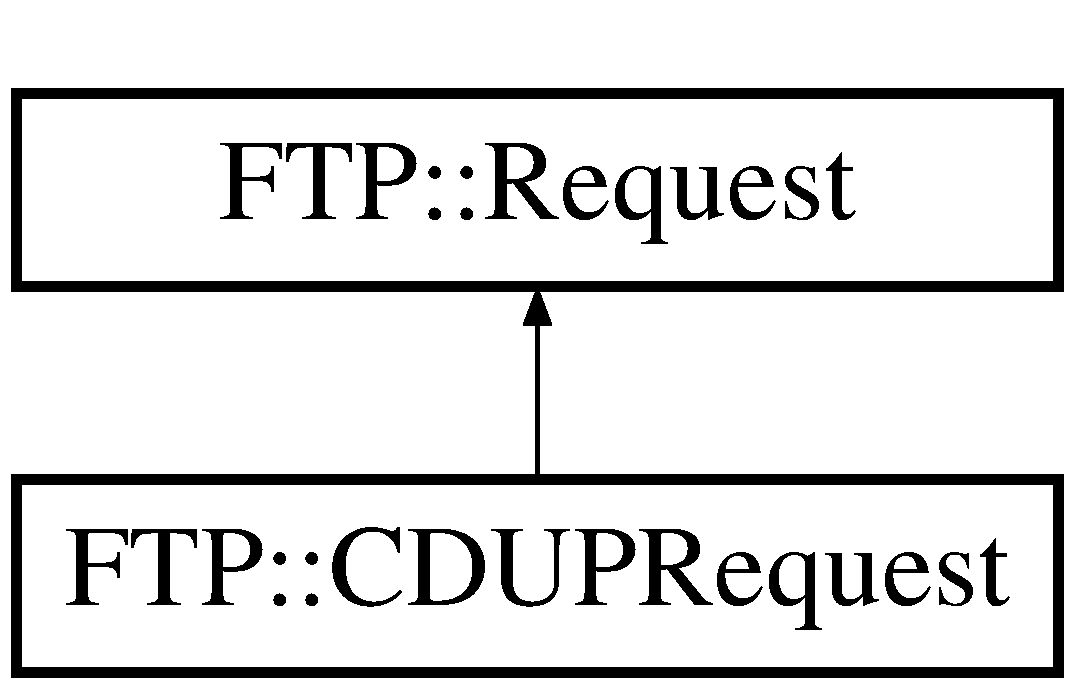
\includegraphics[height=2.000000cm]{classFTP_1_1CDUPRequest}
\end{center}
\end{figure}
\subsection*{Public Member Functions}
\begin{DoxyCompactItemize}
\item 
\hypertarget{classFTP_1_1CDUPRequest_ab15198847bffc2563c46b9ff0b6dd58f}{}\hyperlink{classFTP_1_1CDUPRequest_ab15198847bffc2563c46b9ff0b6dd58f}{C\+D\+U\+P\+Request} ()\label{classFTP_1_1CDUPRequest_ab15198847bffc2563c46b9ff0b6dd58f}

\begin{DoxyCompactList}\small\item\em \hyperlink{classFTP_1_1CDUPRequest}{C\+D\+U\+P\+Request} constructor. \end{DoxyCompactList}\end{DoxyCompactItemize}
\subsection*{Static Public Attributes}
\begin{DoxyCompactItemize}
\item 
\hypertarget{classFTP_1_1CDUPRequest_a3acde3ab0a847af43a10420065dcd535}{}static constexpr const char $\ast$ {\bfseries Command\+Name} = \char`\"{}C\+D\+U\+P\char`\"{}\label{classFTP_1_1CDUPRequest_a3acde3ab0a847af43a10420065dcd535}

\end{DoxyCompactItemize}


\subsection{Detailed Description}
C\+D\+U\+P request. 

Asks the server to set the current directory to its parent folder. 

The documentation for this class was generated from the following file\+:\begin{DoxyCompactItemize}
\item 
C\+:/\+Users/\+Nicolas Cachera/\+Documents/\+Programmation/\+C\+A\+R\+\_\+\+Furet\+T\+P/include/core/message/request/C\+D\+U\+P\+Request.\+h\end{DoxyCompactItemize}

\hypertarget{classFTP_1_1Client}{}\section{F\+T\+P\+:\+:Client Class Reference}
\label{classFTP_1_1Client}\index{F\+T\+P\+::\+Client@{F\+T\+P\+::\+Client}}


\hyperlink{structFTP_1_1User}{User} connection to the Server.  




{\ttfamily \#include $<$Client.\+h$>$}

\subsection*{Public Member Functions}
\begin{DoxyCompactItemize}
\item 
\hyperlink{classFTP_1_1Client_ab611529ac304de5e847df898306b7408}{Client} (\hyperlink{classFTP_1_1FTPServer}{F\+T\+P\+Server} $\ast$server, \hyperlink{classFTP_1_1TCP_1_1Socket}{T\+C\+P\+::\+Socket} \&socket)
\begin{DoxyCompactList}\small\item\em \hyperlink{classFTP_1_1Client}{Client} constructor. \end{DoxyCompactList}\item 
void \hyperlink{classFTP_1_1Client_a260407a0f8d8fe5c7c26b68b5ac2443b}{run} ()
\begin{DoxyCompactList}\small\item\em Runs the connection between \hyperlink{classFTP_1_1Client}{Client} and Server. \end{DoxyCompactList}\item 
\hypertarget{classFTP_1_1Client_a5423cfaf6fc6242ad010c8605df143df}{}bool \hyperlink{classFTP_1_1Client_a5423cfaf6fc6242ad010c8605df143df}{set\+Username} (const std\+::string \&username)\label{classFTP_1_1Client_a5423cfaf6fc6242ad010c8605df143df}

\begin{DoxyCompactList}\small\item\em set username of the client. \end{DoxyCompactList}\item 
bool \hyperlink{classFTP_1_1Client_abfdc9020e33df97a728211b81097113f}{login} (const std\+::string \&password)
\begin{DoxyCompactList}\small\item\em try to loggin with the previous username. \end{DoxyCompactList}\item 
\hypertarget{classFTP_1_1Client_a9d09db3246bb37ee6cd1cb48ae48ec67}{}void \hyperlink{classFTP_1_1Client_a9d09db3246bb37ee6cd1cb48ae48ec67}{reset\+Login} ()\label{classFTP_1_1Client_a9d09db3246bb37ee6cd1cb48ae48ec67}

\begin{DoxyCompactList}\small\item\em Reset login informations. \end{DoxyCompactList}\item 
\hypertarget{classFTP_1_1Client_a027ed05405359ceb55ed5c6a7205ac41}{}void \hyperlink{classFTP_1_1Client_a027ed05405359ceb55ed5c6a7205ac41}{open\+Data\+Connection} ()\label{classFTP_1_1Client_a027ed05405359ceb55ed5c6a7205ac41}

\begin{DoxyCompactList}\small\item\em open new data connection with client \end{DoxyCompactList}\item 
\hypertarget{classFTP_1_1Client_af278600020f84005d320054c55f2d260}{}void \hyperlink{classFTP_1_1Client_af278600020f84005d320054c55f2d260}{send\+To\+Data\+Connection} (const \hyperlink{classFTP_1_1Packet}{Packet} \&packet)\label{classFTP_1_1Client_af278600020f84005d320054c55f2d260}

\begin{DoxyCompactList}\small\item\em send packet on data connection \end{DoxyCompactList}\item 
\hypertarget{classFTP_1_1Client_a8fccfc0518176fb246308f2fb6bc3d62}{}void \hyperlink{classFTP_1_1Client_a8fccfc0518176fb246308f2fb6bc3d62}{receive\+From\+Data\+Connection} (\hyperlink{classFTP_1_1Packet}{Packet} \&packet)\label{classFTP_1_1Client_a8fccfc0518176fb246308f2fb6bc3d62}

\begin{DoxyCompactList}\small\item\em receive packet on data connection \end{DoxyCompactList}\item 
\hypertarget{classFTP_1_1Client_ad8c92ae82b9371bc6da087c77ef0d9d9}{}void \hyperlink{classFTP_1_1Client_ad8c92ae82b9371bc6da087c77ef0d9d9}{close\+Data\+Connection} ()\label{classFTP_1_1Client_ad8c92ae82b9371bc6da087c77ef0d9d9}

\begin{DoxyCompactList}\small\item\em Close the current data connection with the client. \end{DoxyCompactList}\item 
\hypertarget{classFTP_1_1Client_a140d72957c3ee4ed2ecc91bd21ce0c66}{}void \hyperlink{classFTP_1_1Client_a140d72957c3ee4ed2ecc91bd21ce0c66}{set\+Next\+Active\+Connection} (const \hyperlink{classFTP_1_1IP_1_1Address}{I\+P\+::\+Address} \&address, unsigned int port)\label{classFTP_1_1Client_a140d72957c3ee4ed2ecc91bd21ce0c66}

\begin{DoxyCompactList}\small\item\em Set next port and address for active connection. \end{DoxyCompactList}\item 
void \hyperlink{classFTP_1_1Client_a545b1a0a22f36391a6ee8f8563012fa6}{set\+Current\+Directory} (const std\+::string \&pathname)
\begin{DoxyCompactList}\small\item\em Set client current directory from its root directory. \end{DoxyCompactList}\item 
\hypertarget{classFTP_1_1Client_a57cd373e14fbd270455df91ddf0ac0e7}{}void \hyperlink{classFTP_1_1Client_a57cd373e14fbd270455df91ddf0ac0e7}{switch\+Passive\+Mode} ()\label{classFTP_1_1Client_a57cd373e14fbd270455df91ddf0ac0e7}

\begin{DoxyCompactList}\small\item\em Entering in passive mode. \end{DoxyCompactList}\item 
\hypertarget{classFTP_1_1Client_a78f23a9b26bbf98f9fb9b266552d94bb}{}void \hyperlink{classFTP_1_1Client_a78f23a9b26bbf98f9fb9b266552d94bb}{close} ()\label{classFTP_1_1Client_a78f23a9b26bbf98f9fb9b266552d94bb}

\begin{DoxyCompactList}\small\item\em close the client connection and terminate client \end{DoxyCompactList}\item 
\hypertarget{classFTP_1_1Client_abf9b8beac9e9769c78244de4406451d6}{}const \hyperlink{structFTP_1_1User}{User} \& {\bfseries get\+User} () const \label{classFTP_1_1Client_abf9b8beac9e9769c78244de4406451d6}

\item 
\hypertarget{classFTP_1_1Client_ab5f9b53875bb0847045e056a8f9f8073}{}const std\+::string \& {\bfseries get\+Current\+Directory} () const \label{classFTP_1_1Client_ab5f9b53875bb0847045e056a8f9f8073}

\item 
\hypertarget{classFTP_1_1Client_a285e48c50c37c7dd7832a3731182b362}{}\hyperlink{classFTP_1_1TCP_1_1Socket}{T\+C\+P\+::\+Socket} \& {\bfseries get\+Socket} ()\label{classFTP_1_1Client_a285e48c50c37c7dd7832a3731182b362}

\item 
\hypertarget{classFTP_1_1Client_add44878cec59e5f08b68504e0756a87e}{}\hyperlink{classFTP_1_1TCP_1_1Listener}{T\+C\+P\+::\+Listener} \& {\bfseries get\+Passive\+Data\+Listener} ()\label{classFTP_1_1Client_add44878cec59e5f08b68504e0756a87e}

\end{DoxyCompactItemize}


\subsection{Detailed Description}
\hyperlink{structFTP_1_1User}{User} connection to the Server. 

Represents the connection between the user and the server. It\textquotesingle{}s used to receive and send the different packet between the both entities. 

\subsection{Constructor \& Destructor Documentation}
\hypertarget{classFTP_1_1Client_ab611529ac304de5e847df898306b7408}{}\index{F\+T\+P\+::\+Client@{F\+T\+P\+::\+Client}!Client@{Client}}
\index{Client@{Client}!F\+T\+P\+::\+Client@{F\+T\+P\+::\+Client}}
\subsubsection[{Client}]{\setlength{\rightskip}{0pt plus 5cm}F\+T\+P\+::\+Client\+::\+Client (
\begin{DoxyParamCaption}
\item[{{\bf F\+T\+P\+Server} $\ast$}]{server, }
\item[{{\bf T\+C\+P\+::\+Socket} \&}]{socket}
\end{DoxyParamCaption}
)}\label{classFTP_1_1Client_ab611529ac304de5e847df898306b7408}


\hyperlink{classFTP_1_1Client}{Client} constructor. 


\begin{DoxyParams}{Parameters}
{\em server} & Server which the user is connecting. \\
\hline
{\em socket} & \hyperlink{structFTP_1_1User}{User}\textquotesingle{}s socket. \\
\hline
\end{DoxyParams}


\subsection{Member Function Documentation}
\hypertarget{classFTP_1_1Client_abfdc9020e33df97a728211b81097113f}{}\index{F\+T\+P\+::\+Client@{F\+T\+P\+::\+Client}!login@{login}}
\index{login@{login}!F\+T\+P\+::\+Client@{F\+T\+P\+::\+Client}}
\subsubsection[{login}]{\setlength{\rightskip}{0pt plus 5cm}bool F\+T\+P\+::\+Client\+::login (
\begin{DoxyParamCaption}
\item[{const std\+::string \&}]{password}
\end{DoxyParamCaption}
)}\label{classFTP_1_1Client_abfdc9020e33df97a728211b81097113f}


try to loggin with the previous username. 


\begin{DoxyParams}{Parameters}
{\em password} & Password send by the user. \\
\hline
\end{DoxyParams}
\begin{DoxyReturn}{Returns}
True if the client is logged in, false otherwise.
\end{DoxyReturn}
Try to login the client, if an username had been setted. If the password is corresponding with the username, the user is logged in and the method return true. If not, the method return false. \hypertarget{classFTP_1_1Client_a260407a0f8d8fe5c7c26b68b5ac2443b}{}\index{F\+T\+P\+::\+Client@{F\+T\+P\+::\+Client}!run@{run}}
\index{run@{run}!F\+T\+P\+::\+Client@{F\+T\+P\+::\+Client}}
\subsubsection[{run}]{\setlength{\rightskip}{0pt plus 5cm}void F\+T\+P\+::\+Client\+::run (
\begin{DoxyParamCaption}
{}
\end{DoxyParamCaption}
)}\label{classFTP_1_1Client_a260407a0f8d8fe5c7c26b68b5ac2443b}


Runs the connection between \hyperlink{classFTP_1_1Client}{Client} and Server. 

Runs the connection between \hyperlink{classFTP_1_1Client}{Client} and Server while the socket is open. Receives each packet from the user and interprets them. If the received packet is a known request, it calls the \hyperlink{classFTP_1_1RequestHandler}{Request\+Handler}, else it sends an unimplemented command packet. \hypertarget{classFTP_1_1Client_a545b1a0a22f36391a6ee8f8563012fa6}{}\index{F\+T\+P\+::\+Client@{F\+T\+P\+::\+Client}!set\+Current\+Directory@{set\+Current\+Directory}}
\index{set\+Current\+Directory@{set\+Current\+Directory}!F\+T\+P\+::\+Client@{F\+T\+P\+::\+Client}}
\subsubsection[{set\+Current\+Directory}]{\setlength{\rightskip}{0pt plus 5cm}void F\+T\+P\+::\+Client\+::set\+Current\+Directory (
\begin{DoxyParamCaption}
\item[{const std\+::string \&}]{pathname}
\end{DoxyParamCaption}
)}\label{classFTP_1_1Client_a545b1a0a22f36391a6ee8f8563012fa6}


Set client current directory from its root directory. 

This pathname need to be absolute considering client root directory as root 

The documentation for this class was generated from the following file\+:\begin{DoxyCompactItemize}
\item 
C\+:/\+Users/\+Nicolas Cachera/\+Documents/\+Programmation/\+C\+A\+R\+\_\+\+Furet\+T\+P/include/core/Client.\+h\end{DoxyCompactItemize}

\input{classCWDPRequest}
\hypertarget{classFTP_1_1CWDRequest}{}\section{F\+T\+P\+:\+:C\+W\+D\+Request Class Reference}
\label{classFTP_1_1CWDRequest}\index{F\+T\+P\+::\+C\+W\+D\+Request@{F\+T\+P\+::\+C\+W\+D\+Request}}


C\+W\+D request.  




{\ttfamily \#include $<$C\+W\+D\+Request.\+h$>$}

Inheritance diagram for F\+T\+P\+:\+:C\+W\+D\+Request\+:\begin{figure}[H]
\begin{center}
\leavevmode
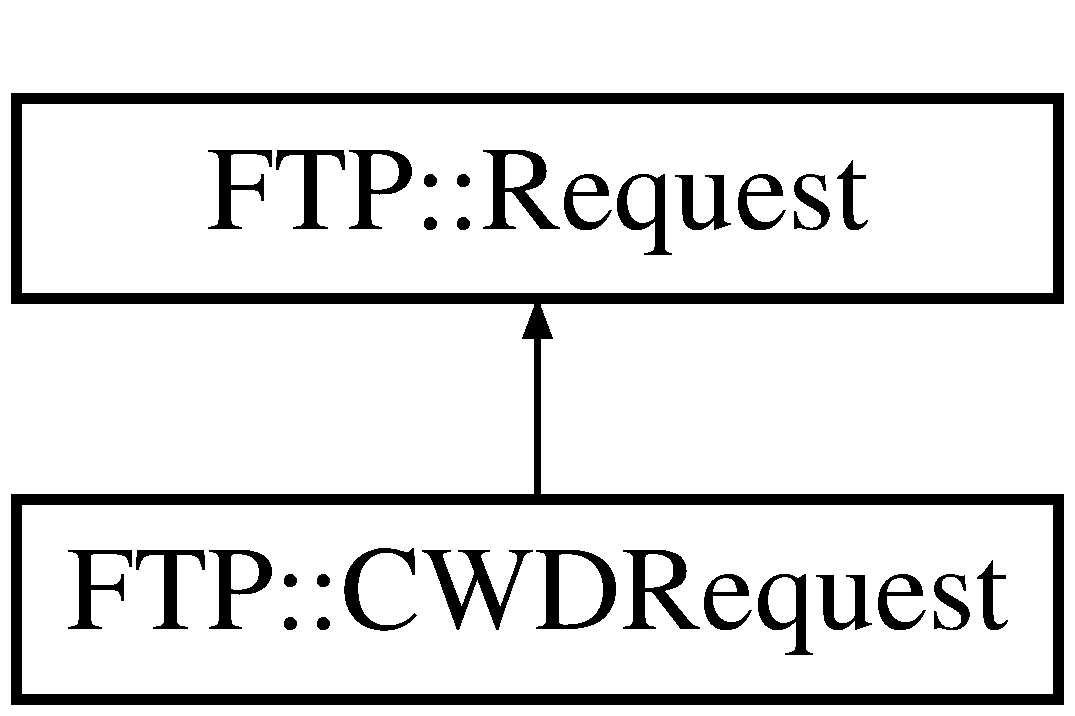
\includegraphics[height=2.000000cm]{classFTP_1_1CWDRequest}
\end{center}
\end{figure}
\subsection*{Public Member Functions}
\begin{DoxyCompactItemize}
\item 
\hyperlink{classFTP_1_1CWDRequest_a091feea182bab2dd9a7b4fd5d4d3decc}{C\+W\+D\+Request} (const std\+::string \&directory)
\begin{DoxyCompactList}\small\item\em \hyperlink{classFTP_1_1CWDRequest}{C\+W\+D\+Request} constructor. \end{DoxyCompactList}\item 
\hypertarget{classFTP_1_1CWDRequest_a1206a80f13f5690af449ddc409bbee95}{}const std\+::string \& {\bfseries get\+Directory} () const \label{classFTP_1_1CWDRequest_a1206a80f13f5690af449ddc409bbee95}

\end{DoxyCompactItemize}
\subsection*{Static Public Attributes}
\begin{DoxyCompactItemize}
\item 
\hypertarget{classFTP_1_1CWDRequest_a9985962b0f7a8b28c49020d37e509b7d}{}static constexpr const char $\ast$ {\bfseries Command\+Name} = \char`\"{}C\+W\+D\char`\"{}\label{classFTP_1_1CWDRequest_a9985962b0f7a8b28c49020d37e509b7d}

\end{DoxyCompactItemize}


\subsection{Detailed Description}
C\+W\+D request. 

Asks the server to change the current directory. Accept absolute and relative path 

\subsection{Constructor \& Destructor Documentation}
\hypertarget{classFTP_1_1CWDRequest_a091feea182bab2dd9a7b4fd5d4d3decc}{}\index{F\+T\+P\+::\+C\+W\+D\+Request@{F\+T\+P\+::\+C\+W\+D\+Request}!C\+W\+D\+Request@{C\+W\+D\+Request}}
\index{C\+W\+D\+Request@{C\+W\+D\+Request}!F\+T\+P\+::\+C\+W\+D\+Request@{F\+T\+P\+::\+C\+W\+D\+Request}}
\subsubsection[{C\+W\+D\+Request}]{\setlength{\rightskip}{0pt plus 5cm}F\+T\+P\+::\+C\+W\+D\+Request\+::\+C\+W\+D\+Request (
\begin{DoxyParamCaption}
\item[{const std\+::string \&}]{directory}
\end{DoxyParamCaption}
)}\label{classFTP_1_1CWDRequest_a091feea182bab2dd9a7b4fd5d4d3decc}


\hyperlink{classFTP_1_1CWDRequest}{C\+W\+D\+Request} constructor. 


\begin{DoxyParams}{Parameters}
{\em directory} & New current directory\\
\hline
\end{DoxyParams}
The directory needs to exist 

The documentation for this class was generated from the following file\+:\begin{DoxyCompactItemize}
\item 
C\+:/\+Users/\+Nicolas Cachera/\+Documents/\+Programmation/\+C\+A\+R\+\_\+\+Furet\+T\+P/include/core/message/request/C\+W\+D\+Request.\+h\end{DoxyCompactItemize}

\hypertarget{classFTP_1_1Directory}{}\section{F\+T\+P\+:\+:Directory Class Reference}
\label{classFTP_1_1Directory}\index{F\+T\+P\+::\+Directory@{F\+T\+P\+::\+Directory}}


\hyperlink{classFTP_1_1Directory}{Directory} management classx.  




{\ttfamily \#include $<$Directory.\+h$>$}

\subsection*{Classes}
\begin{DoxyCompactItemize}
\item 
class \hyperlink{structFTP_1_1Directory_1_1Entry}{Entry}
\begin{DoxyCompactList}\small\item\em \hyperlink{structFTP_1_1Directory_1_1Entry}{Entry} in directory. \end{DoxyCompactList}\end{DoxyCompactItemize}
\subsection*{Public Member Functions}
\begin{DoxyCompactItemize}
\item 
void \hyperlink{classFTP_1_1Directory_a55f609eb353e6f9806c19e93e294ac0a}{open} (std\+::string pathname)
\begin{DoxyCompactList}\small\item\em open a directory \end{DoxyCompactList}\item 
void \hyperlink{classFTP_1_1Directory_a2030a6e209fbe90537db216839eb6c75}{list} (std\+::vector$<$ \hyperlink{structFTP_1_1Directory_1_1Entry}{Entry} $>$ \&entries)
\begin{DoxyCompactList}\small\item\em list the directory contents. Need previously be openend \end{DoxyCompactList}\item 
\hypertarget{classFTP_1_1Directory_abb5502a657390ea09207d51494213b27}{}void \hyperlink{classFTP_1_1Directory_abb5502a657390ea09207d51494213b27}{close} ()\label{classFTP_1_1Directory_abb5502a657390ea09207d51494213b27}

\begin{DoxyCompactList}\small\item\em close directory \end{DoxyCompactList}\end{DoxyCompactItemize}


\subsection{Detailed Description}
\hyperlink{classFTP_1_1Directory}{Directory} management classx. 

Enscapsulate C directory reader functions. Allow to list the content directory 

\subsection{Member Function Documentation}
\hypertarget{classFTP_1_1Directory_a2030a6e209fbe90537db216839eb6c75}{}\index{F\+T\+P\+::\+Directory@{F\+T\+P\+::\+Directory}!list@{list}}
\index{list@{list}!F\+T\+P\+::\+Directory@{F\+T\+P\+::\+Directory}}
\subsubsection[{list}]{\setlength{\rightskip}{0pt plus 5cm}void F\+T\+P\+::\+Directory\+::list (
\begin{DoxyParamCaption}
\item[{std\+::vector$<$ {\bf Entry} $>$ \&}]{entries}
\end{DoxyParamCaption}
)}\label{classFTP_1_1Directory_a2030a6e209fbe90537db216839eb6c75}


list the directory contents. Need previously be openend 


\begin{DoxyParams}{Parameters}
{\em entries} & \+: a vector which be fill with all the entries of the opened directory \\
\hline
\end{DoxyParams}
\hypertarget{classFTP_1_1Directory_a55f609eb353e6f9806c19e93e294ac0a}{}\index{F\+T\+P\+::\+Directory@{F\+T\+P\+::\+Directory}!open@{open}}
\index{open@{open}!F\+T\+P\+::\+Directory@{F\+T\+P\+::\+Directory}}
\subsubsection[{open}]{\setlength{\rightskip}{0pt plus 5cm}void F\+T\+P\+::\+Directory\+::open (
\begin{DoxyParamCaption}
\item[{std\+::string}]{pathname}
\end{DoxyParamCaption}
)}\label{classFTP_1_1Directory_a55f609eb353e6f9806c19e93e294ac0a}


open a directory 


\begin{DoxyParams}{Parameters}
{\em pathname} & of the directory \\
\hline
\end{DoxyParams}


The documentation for this class was generated from the following file\+:\begin{DoxyCompactItemize}
\item 
C\+:/\+Users/\+Nicolas Cachera/\+Documents/\+Programmation/\+C\+A\+R\+\_\+\+Furet\+T\+P/include/system/Directory.\+h\end{DoxyCompactItemize}

\hypertarget{structFTP_1_1Directory_1_1Entry}{}\section{F\+T\+P\+:\+:Directory\+:\+:Entry Class Reference}
\label{structFTP_1_1Directory_1_1Entry}\index{F\+T\+P\+::\+Directory\+::\+Entry@{F\+T\+P\+::\+Directory\+::\+Entry}}


\hyperlink{structFTP_1_1Directory_1_1Entry}{Entry} in directory.  




{\ttfamily \#include $<$Directory.\+h$>$}

\subsection*{Public Attributes}
\begin{DoxyCompactItemize}
\item 
\hypertarget{structFTP_1_1Directory_1_1Entry_aac9c20aeb62b9a48ebd1e8bfb897aabf}{}std\+::string \hyperlink{structFTP_1_1Directory_1_1Entry_aac9c20aeb62b9a48ebd1e8bfb897aabf}{permission}\label{structFTP_1_1Directory_1_1Entry_aac9c20aeb62b9a48ebd1e8bfb897aabf}

\begin{DoxyCompactList}\small\item\em file permission in Unix presentation (like -\/rwxr-\/x---) \end{DoxyCompactList}\item 
\hypertarget{structFTP_1_1Directory_1_1Entry_a75b6770d2c8fd215755a7ad5f3187e25}{}unsigned int \hyperlink{structFTP_1_1Directory_1_1Entry_a75b6770d2c8fd215755a7ad5f3187e25}{size}\label{structFTP_1_1Directory_1_1Entry_a75b6770d2c8fd215755a7ad5f3187e25}

\begin{DoxyCompactList}\small\item\em file size \end{DoxyCompactList}\item 
\hypertarget{structFTP_1_1Directory_1_1Entry_a7476d45d4a0267cbf9e708bbc5bdc3e1}{}std\+::string \hyperlink{structFTP_1_1Directory_1_1Entry_a7476d45d4a0267cbf9e708bbc5bdc3e1}{name}\label{structFTP_1_1Directory_1_1Entry_a7476d45d4a0267cbf9e708bbc5bdc3e1}

\begin{DoxyCompactList}\small\item\em file name \end{DoxyCompactList}\item 
\hypertarget{structFTP_1_1Directory_1_1Entry_adc85896558570dd9d34709848804ce78}{}std\+::string \hyperlink{structFTP_1_1Directory_1_1Entry_adc85896558570dd9d34709848804ce78}{last\+Modification}\label{structFTP_1_1Directory_1_1Entry_adc85896558570dd9d34709848804ce78}

\begin{DoxyCompactList}\small\item\em last modification date in format month day hh\+:mm \end{DoxyCompactList}\end{DoxyCompactItemize}


\subsection{Detailed Description}
\hyperlink{structFTP_1_1Directory_1_1Entry}{Entry} in directory. 

Structure which contains entry information 

The documentation for this class was generated from the following file\+:\begin{DoxyCompactItemize}
\item 
C\+:/\+Users/\+Nicolas Cachera/\+Documents/\+Programmation/\+C\+A\+R\+\_\+\+Furet\+T\+P/include/system/Directory.\+h\end{DoxyCompactItemize}

\hypertarget{classFTP_1_1Exception}{}\section{F\+T\+P\+:\+:Exception Class Reference}
\label{classFTP_1_1Exception}\index{F\+T\+P\+::\+Exception@{F\+T\+P\+::\+Exception}}


Basic exception.  




{\ttfamily \#include $<$Exception.\+h$>$}

Inheritance diagram for F\+T\+P\+:\+:Exception\+:\begin{figure}[H]
\begin{center}
\leavevmode
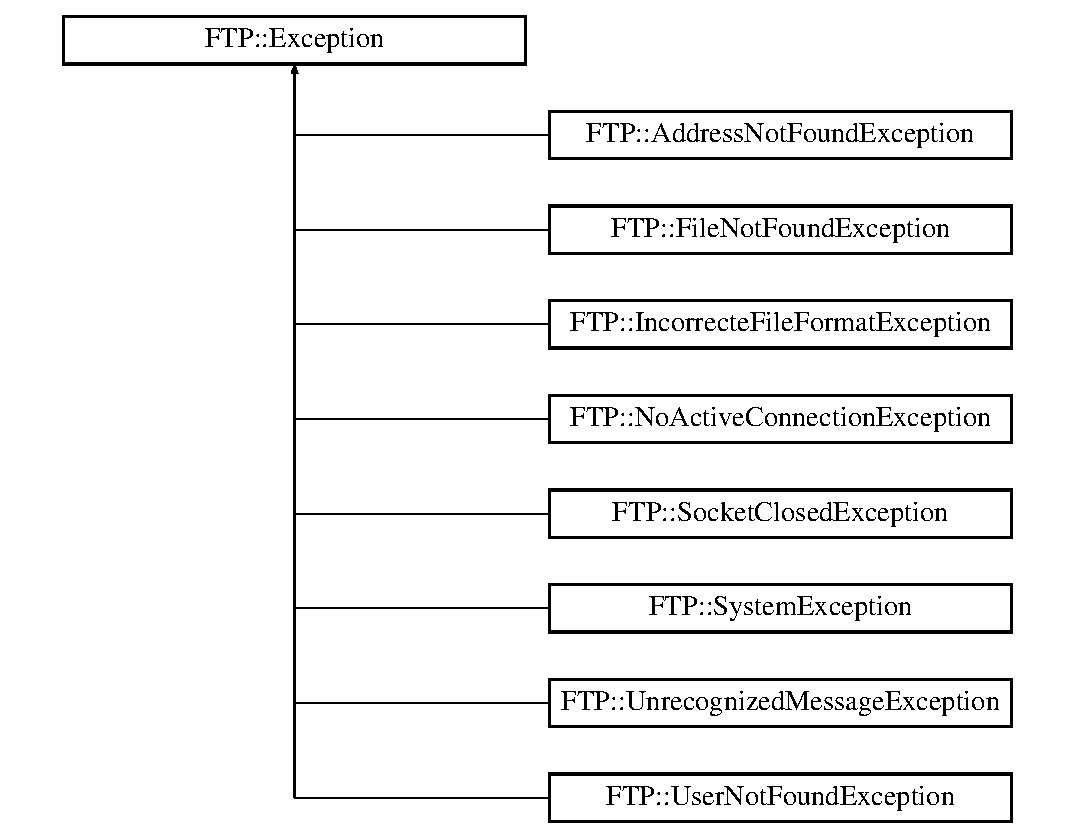
\includegraphics[height=9.000000cm]{classFTP_1_1Exception}
\end{center}
\end{figure}
\subsection*{Public Member Functions}
\begin{DoxyCompactItemize}
\item 
\hypertarget{classFTP_1_1Exception_a2451744502231316fb25c76b9d0e4ad0}{}\hyperlink{classFTP_1_1Exception_a2451744502231316fb25c76b9d0e4ad0}{Exception} ()\label{classFTP_1_1Exception_a2451744502231316fb25c76b9d0e4ad0}

\begin{DoxyCompactList}\small\item\em \hyperlink{classFTP_1_1Exception}{Exception} constructor. \end{DoxyCompactList}\item 
\hyperlink{classFTP_1_1Exception_a2c62e4f58bf71065327a509d87cd1ae0}{Exception} (const std\+::string \&message)
\begin{DoxyCompactList}\small\item\em \hyperlink{classFTP_1_1Exception}{Exception} constructor. \end{DoxyCompactList}\item 
void \hyperlink{classFTP_1_1Exception_a462325fec2828a1cc5d06b9b1994dc49}{set\+Localisation} (const char $\ast$file, int line)
\begin{DoxyCompactList}\small\item\em Set error localisation in a file. \end{DoxyCompactList}\item 
\hypertarget{classFTP_1_1Exception_ab8184759911a05c6ff47b0807237fae9}{}const std\+::string \& {\bfseries get\+Message} () const   throw ()\label{classFTP_1_1Exception_ab8184759911a05c6ff47b0807237fae9}

\item 
\hypertarget{classFTP_1_1Exception_a16f83d3adfebfb58402c761d337e7ff0}{}const char $\ast$ {\bfseries get\+File} () const   throw ()\label{classFTP_1_1Exception_a16f83d3adfebfb58402c761d337e7ff0}

\item 
\hypertarget{classFTP_1_1Exception_a76b9ea580b17dc54d29b1e42525711c2}{}int {\bfseries get\+Line} () const   throw ()\label{classFTP_1_1Exception_a76b9ea580b17dc54d29b1e42525711c2}

\end{DoxyCompactItemize}


\subsection{Detailed Description}
Basic exception. 

\subsection{Constructor \& Destructor Documentation}
\hypertarget{classFTP_1_1Exception_a2c62e4f58bf71065327a509d87cd1ae0}{}\index{F\+T\+P\+::\+Exception@{F\+T\+P\+::\+Exception}!Exception@{Exception}}
\index{Exception@{Exception}!F\+T\+P\+::\+Exception@{F\+T\+P\+::\+Exception}}
\subsubsection[{Exception}]{\setlength{\rightskip}{0pt plus 5cm}F\+T\+P\+::\+Exception\+::\+Exception (
\begin{DoxyParamCaption}
\item[{const std\+::string \&}]{message}
\end{DoxyParamCaption}
)}\label{classFTP_1_1Exception_a2c62e4f58bf71065327a509d87cd1ae0}


\hyperlink{classFTP_1_1Exception}{Exception} constructor. 


\begin{DoxyParams}{Parameters}
{\em message} & A message to print \\
\hline
\end{DoxyParams}


\subsection{Member Function Documentation}
\hypertarget{classFTP_1_1Exception_a462325fec2828a1cc5d06b9b1994dc49}{}\index{F\+T\+P\+::\+Exception@{F\+T\+P\+::\+Exception}!set\+Localisation@{set\+Localisation}}
\index{set\+Localisation@{set\+Localisation}!F\+T\+P\+::\+Exception@{F\+T\+P\+::\+Exception}}
\subsubsection[{set\+Localisation}]{\setlength{\rightskip}{0pt plus 5cm}void F\+T\+P\+::\+Exception\+::set\+Localisation (
\begin{DoxyParamCaption}
\item[{const char $\ast$}]{file, }
\item[{int}]{line}
\end{DoxyParamCaption}
)}\label{classFTP_1_1Exception_a462325fec2828a1cc5d06b9b1994dc49}


Set error localisation in a file. 


\begin{DoxyParams}{Parameters}
{\em file} & The file which contains the error \\
\hline
{\em line} & The line which contains the error \\
\hline
\end{DoxyParams}


The documentation for this class was generated from the following file\+:\begin{DoxyCompactItemize}
\item 
C\+:/\+Users/\+Nicolas Cachera/\+Documents/\+Programmation/\+C\+A\+R\+\_\+\+Furet\+T\+P/include/exception/Exception.\+h\end{DoxyCompactItemize}

\hypertarget{classFTP_1_1FeatRequest}{}\section{F\+T\+P\+:\+:Feat\+Request Class Reference}
\label{classFTP_1_1FeatRequest}\index{F\+T\+P\+::\+Feat\+Request@{F\+T\+P\+::\+Feat\+Request}}


Feat request.  




{\ttfamily \#include $<$Feat\+Request.\+h$>$}

Inheritance diagram for F\+T\+P\+:\+:Feat\+Request\+:\begin{figure}[H]
\begin{center}
\leavevmode
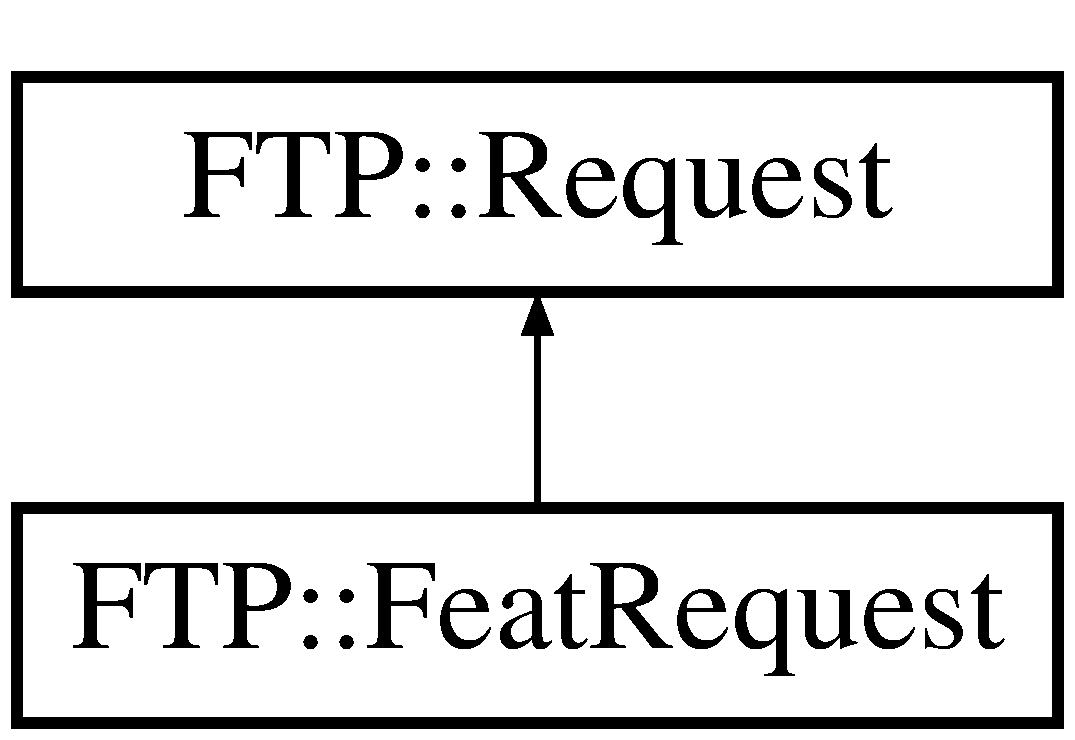
\includegraphics[height=2.000000cm]{classFTP_1_1FeatRequest}
\end{center}
\end{figure}
\subsection*{Public Member Functions}
\begin{DoxyCompactItemize}
\item 
\hypertarget{classFTP_1_1FeatRequest_a3f4a0e055a9fcacd680c8550f1410229}{}\hyperlink{classFTP_1_1FeatRequest_a3f4a0e055a9fcacd680c8550f1410229}{Feat\+Request} ()\label{classFTP_1_1FeatRequest_a3f4a0e055a9fcacd680c8550f1410229}

\begin{DoxyCompactList}\small\item\em \hyperlink{classFTP_1_1FeatRequest}{Feat\+Request} constructor. \end{DoxyCompactList}\end{DoxyCompactItemize}
\subsection*{Static Public Attributes}
\begin{DoxyCompactItemize}
\item 
\hypertarget{classFTP_1_1FeatRequest_aa42ff5dc78f3d80b1944ee80f0340017}{}static constexpr const char $\ast$ {\bfseries Command\+Name} = \char`\"{}F\+E\+A\+T\char`\"{}\label{classFTP_1_1FeatRequest_aa42ff5dc78f3d80b1944ee80f0340017}

\end{DoxyCompactItemize}


\subsection{Detailed Description}
Feat request. 

\hyperlink{classFTP_1_1Request}{Request} sent to know extra command supported by server undefined in R\+F\+C 959. 

The documentation for this class was generated from the following file\+:\begin{DoxyCompactItemize}
\item 
C\+:/\+Users/\+Nicolas Cachera/\+Documents/\+Programmation/\+C\+A\+R\+\_\+\+Furet\+T\+P/include/core/message/request/Feat\+Request.\+h\end{DoxyCompactItemize}

\hypertarget{classFTP_1_1FileNotFoundException}{}\section{F\+T\+P\+:\+:File\+Not\+Found\+Exception Class Reference}
\label{classFTP_1_1FileNotFoundException}\index{F\+T\+P\+::\+File\+Not\+Found\+Exception@{F\+T\+P\+::\+File\+Not\+Found\+Exception}}


\hyperlink{classFTP_1_1Exception}{Exception} launched when a file is needed but not found.  




{\ttfamily \#include $<$File\+Not\+Found\+Exception.\+h$>$}

Inheritance diagram for F\+T\+P\+:\+:File\+Not\+Found\+Exception\+:\begin{figure}[H]
\begin{center}
\leavevmode
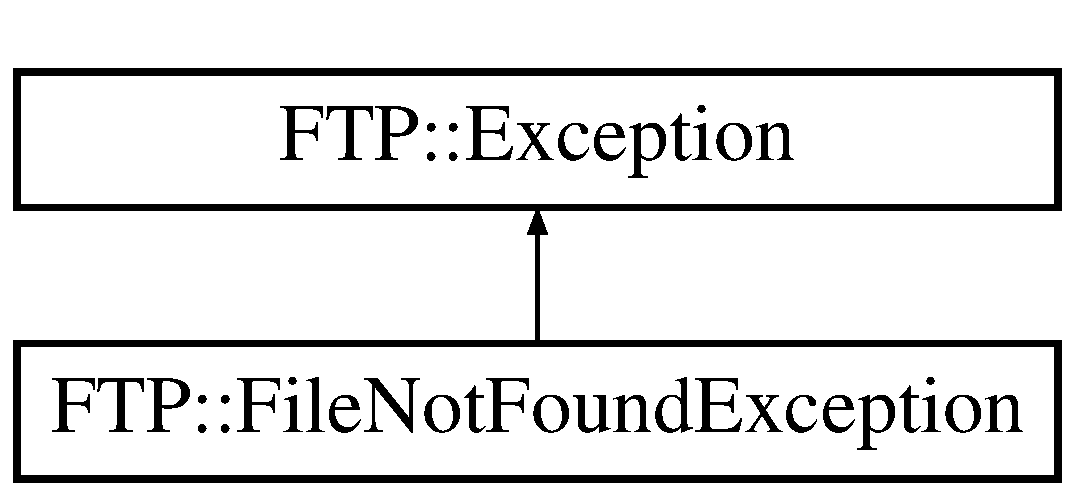
\includegraphics[height=2.000000cm]{classFTP_1_1FileNotFoundException}
\end{center}
\end{figure}
\subsection*{Public Member Functions}
\begin{DoxyCompactItemize}
\item 
\hyperlink{classFTP_1_1FileNotFoundException_aad708c1cca717cbff7eb2ce33978536e}{File\+Not\+Found\+Exception} (const std\+::string \&file)
\begin{DoxyCompactList}\small\item\em \hyperlink{classFTP_1_1FileNotFoundException}{File\+Not\+Found\+Exception} constructor. \end{DoxyCompactList}\end{DoxyCompactItemize}


\subsection{Detailed Description}
\hyperlink{classFTP_1_1Exception}{Exception} launched when a file is needed but not found. 

\subsection{Constructor \& Destructor Documentation}
\hypertarget{classFTP_1_1FileNotFoundException_aad708c1cca717cbff7eb2ce33978536e}{}\index{F\+T\+P\+::\+File\+Not\+Found\+Exception@{F\+T\+P\+::\+File\+Not\+Found\+Exception}!File\+Not\+Found\+Exception@{File\+Not\+Found\+Exception}}
\index{File\+Not\+Found\+Exception@{File\+Not\+Found\+Exception}!F\+T\+P\+::\+File\+Not\+Found\+Exception@{F\+T\+P\+::\+File\+Not\+Found\+Exception}}
\subsubsection[{File\+Not\+Found\+Exception}]{\setlength{\rightskip}{0pt plus 5cm}F\+T\+P\+::\+File\+Not\+Found\+Exception\+::\+File\+Not\+Found\+Exception (
\begin{DoxyParamCaption}
\item[{const std\+::string \&}]{file}
\end{DoxyParamCaption}
)}\label{classFTP_1_1FileNotFoundException_aad708c1cca717cbff7eb2ce33978536e}


\hyperlink{classFTP_1_1FileNotFoundException}{File\+Not\+Found\+Exception} constructor. 


\begin{DoxyParams}{Parameters}
{\em file} & The file which is not found \\
\hline
\end{DoxyParams}


The documentation for this class was generated from the following file\+:\begin{DoxyCompactItemize}
\item 
C\+:/\+Users/\+Nicolas Cachera/\+Documents/\+Programmation/\+C\+A\+R\+\_\+\+Furet\+T\+P/include/exception/File\+Not\+Found\+Exception.\+h\end{DoxyCompactItemize}

\hypertarget{classFTP_1_1FTPServer}{}\section{F\+T\+P\+:\+:F\+T\+P\+Server Class Reference}
\label{classFTP_1_1FTPServer}\index{F\+T\+P\+::\+F\+T\+P\+Server@{F\+T\+P\+::\+F\+T\+P\+Server}}


Represents the F\+T\+P Server.  




{\ttfamily \#include $<$F\+T\+P\+Server.\+h$>$}

\subsection*{Public Member Functions}
\begin{DoxyCompactItemize}
\item 
\hyperlink{classFTP_1_1FTPServer_a8ea3b0bab4f4991de8060c7741ef84b2}{F\+T\+P\+Server} (const \hyperlink{classFTP_1_1ServerConfiguration}{Server\+Configuration} \&configuration)
\begin{DoxyCompactList}\small\item\em \hyperlink{classFTP_1_1FTPServer}{F\+T\+P\+Server} constructor. \end{DoxyCompactList}\item 
void \hyperlink{classFTP_1_1FTPServer_ac484c041ac5c602c6a0e5eb77b4c2828}{run} ()
\begin{DoxyCompactList}\small\item\em run the server while the application is launched \end{DoxyCompactList}\item 
\hypertarget{classFTP_1_1FTPServer_a3606447f498e487d2ab498dfddb62422}{}void \hyperlink{classFTP_1_1FTPServer_a3606447f498e487d2ab498dfddb62422}{close} ()\label{classFTP_1_1FTPServer_a3606447f498e487d2ab498dfddb62422}

\begin{DoxyCompactList}\small\item\em Close the server and every connection. \end{DoxyCompactList}\item 
\hypertarget{classFTP_1_1FTPServer_a505cd213609eccfa11d806562010d13f}{}const \hyperlink{classFTP_1_1ServerConfiguration}{Server\+Configuration} \& {\bfseries get\+Configuration} () const \label{classFTP_1_1FTPServer_a505cd213609eccfa11d806562010d13f}

\end{DoxyCompactItemize}


\subsection{Detailed Description}
Represents the F\+T\+P Server. 

Represents the F\+T\+P Server. It receives user connections then create a \hyperlink{classFTP_1_1Client}{Client} instance for each of them. 

\subsection{Constructor \& Destructor Documentation}
\hypertarget{classFTP_1_1FTPServer_a8ea3b0bab4f4991de8060c7741ef84b2}{}\index{F\+T\+P\+::\+F\+T\+P\+Server@{F\+T\+P\+::\+F\+T\+P\+Server}!F\+T\+P\+Server@{F\+T\+P\+Server}}
\index{F\+T\+P\+Server@{F\+T\+P\+Server}!F\+T\+P\+::\+F\+T\+P\+Server@{F\+T\+P\+::\+F\+T\+P\+Server}}
\subsubsection[{F\+T\+P\+Server}]{\setlength{\rightskip}{0pt plus 5cm}F\+T\+P\+::\+F\+T\+P\+Server\+::\+F\+T\+P\+Server (
\begin{DoxyParamCaption}
\item[{const {\bf Server\+Configuration} \&}]{configuration}
\end{DoxyParamCaption}
)}\label{classFTP_1_1FTPServer_a8ea3b0bab4f4991de8060c7741ef84b2}


\hyperlink{classFTP_1_1FTPServer}{F\+T\+P\+Server} constructor. 


\begin{DoxyParams}{Parameters}
{\em configuration} & Configuration of the server. \\
\hline
\end{DoxyParams}


\subsection{Member Function Documentation}
\hypertarget{classFTP_1_1FTPServer_ac484c041ac5c602c6a0e5eb77b4c2828}{}\index{F\+T\+P\+::\+F\+T\+P\+Server@{F\+T\+P\+::\+F\+T\+P\+Server}!run@{run}}
\index{run@{run}!F\+T\+P\+::\+F\+T\+P\+Server@{F\+T\+P\+::\+F\+T\+P\+Server}}
\subsubsection[{run}]{\setlength{\rightskip}{0pt plus 5cm}void F\+T\+P\+::\+F\+T\+P\+Server\+::run (
\begin{DoxyParamCaption}
{}
\end{DoxyParamCaption}
)}\label{classFTP_1_1FTPServer_ac484c041ac5c602c6a0e5eb77b4c2828}


run the server while the application is launched 

Creates a \hyperlink{classFTP_1_1Client}{Client} instance each time the server receives a user connection and create a new thread. 

The documentation for this class was generated from the following file\+:\begin{DoxyCompactItemize}
\item 
C\+:/\+Users/\+Nicolas Cachera/\+Documents/\+Programmation/\+C\+A\+R\+\_\+\+Furet\+T\+P/include/core/F\+T\+P\+Server.\+h\end{DoxyCompactItemize}

\hypertarget{classFTP_1_1IncorrecteFileFormatException}{}\section{F\+T\+P\+:\+:Incorrecte\+File\+Format\+Exception Class Reference}
\label{classFTP_1_1IncorrecteFileFormatException}\index{F\+T\+P\+::\+Incorrecte\+File\+Format\+Exception@{F\+T\+P\+::\+Incorrecte\+File\+Format\+Exception}}


\hyperlink{classFTP_1_1Exception}{Exception} launched when a file format is incorrect.  




{\ttfamily \#include $<$Incorrecte\+File\+Format\+Exception.\+h$>$}

Inheritance diagram for F\+T\+P\+:\+:Incorrecte\+File\+Format\+Exception\+:\begin{figure}[H]
\begin{center}
\leavevmode
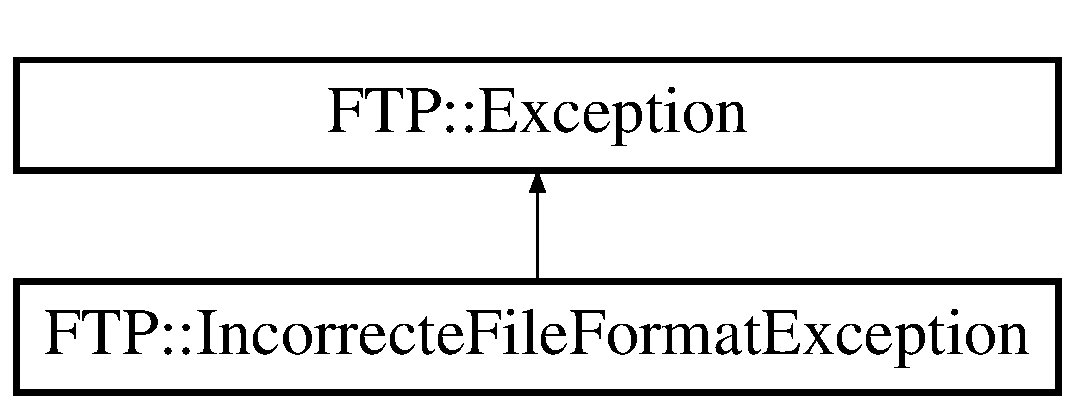
\includegraphics[height=2.000000cm]{classFTP_1_1IncorrecteFileFormatException}
\end{center}
\end{figure}
\subsection*{Public Member Functions}
\begin{DoxyCompactItemize}
\item 
\hyperlink{classFTP_1_1IncorrecteFileFormatException_a0ade738f890878daee4f89a1447cb590}{Incorrecte\+File\+Format\+Exception} (const std\+::string \&message, unsigned int line, const std\+::string \&file)
\begin{DoxyCompactList}\small\item\em \hyperlink{classFTP_1_1IncorrecteFileFormatException}{Incorrecte\+File\+Format\+Exception} constructor. \end{DoxyCompactList}\end{DoxyCompactItemize}


\subsection{Detailed Description}
\hyperlink{classFTP_1_1Exception}{Exception} launched when a file format is incorrect. 

\subsection{Constructor \& Destructor Documentation}
\hypertarget{classFTP_1_1IncorrecteFileFormatException_a0ade738f890878daee4f89a1447cb590}{}\index{F\+T\+P\+::\+Incorrecte\+File\+Format\+Exception@{F\+T\+P\+::\+Incorrecte\+File\+Format\+Exception}!Incorrecte\+File\+Format\+Exception@{Incorrecte\+File\+Format\+Exception}}
\index{Incorrecte\+File\+Format\+Exception@{Incorrecte\+File\+Format\+Exception}!F\+T\+P\+::\+Incorrecte\+File\+Format\+Exception@{F\+T\+P\+::\+Incorrecte\+File\+Format\+Exception}}
\subsubsection[{Incorrecte\+File\+Format\+Exception}]{\setlength{\rightskip}{0pt plus 5cm}F\+T\+P\+::\+Incorrecte\+File\+Format\+Exception\+::\+Incorrecte\+File\+Format\+Exception (
\begin{DoxyParamCaption}
\item[{const std\+::string \&}]{message, }
\item[{unsigned int}]{line, }
\item[{const std\+::string \&}]{file}
\end{DoxyParamCaption}
)}\label{classFTP_1_1IncorrecteFileFormatException_a0ade738f890878daee4f89a1447cb590}


\hyperlink{classFTP_1_1IncorrecteFileFormatException}{Incorrecte\+File\+Format\+Exception} constructor. 


\begin{DoxyParams}{Parameters}
{\em message} & A message to print \\
\hline
{\em line} & The line of the error in the file \\
\hline
{\em file} & The name of the incorrect file \\
\hline
\end{DoxyParams}


The documentation for this class was generated from the following file\+:\begin{DoxyCompactItemize}
\item 
C\+:/\+Users/\+Nicolas Cachera/\+Documents/\+Programmation/\+C\+A\+R\+\_\+\+Furet\+T\+P/include/exception/Incorrecte\+File\+Format\+Exception.\+h\end{DoxyCompactItemize}

\hypertarget{classFTP_1_1TCP_1_1Listener}{}\section{F\+T\+P\+:\+:T\+C\+P\+:\+:Listener Class Reference}
\label{classFTP_1_1TCP_1_1Listener}\index{F\+T\+P\+::\+T\+C\+P\+::\+Listener@{F\+T\+P\+::\+T\+C\+P\+::\+Listener}}


T\+C\+P socket listener.  




{\ttfamily \#include $<$Listener.\+h$>$}

\subsection*{Public Member Functions}
\begin{DoxyCompactItemize}
\item 
\hypertarget{classFTP_1_1TCP_1_1Listener_a69e4e544dd49c56e1d2cac10a314d90a}{}\hyperlink{classFTP_1_1TCP_1_1Listener_a69e4e544dd49c56e1d2cac10a314d90a}{Listener} ()\label{classFTP_1_1TCP_1_1Listener_a69e4e544dd49c56e1d2cac10a314d90a}

\begin{DoxyCompactList}\small\item\em create a listener. \end{DoxyCompactList}\item 
\hypertarget{classFTP_1_1TCP_1_1Listener_aafa6fa407abdfd638db25fb0d610252e}{}void \hyperlink{classFTP_1_1TCP_1_1Listener_aafa6fa407abdfd638db25fb0d610252e}{listen} (unsigned int port)\label{classFTP_1_1TCP_1_1Listener_aafa6fa407abdfd638db25fb0d610252e}

\begin{DoxyCompactList}\small\item\em bind a port for listen client connections \end{DoxyCompactList}\item 
\hypertarget{classFTP_1_1TCP_1_1Listener_abd151bda4845bec6533c75667499c21f}{}unsigned int \hyperlink{classFTP_1_1TCP_1_1Listener_abd151bda4845bec6533c75667499c21f}{listen} ()\label{classFTP_1_1TCP_1_1Listener_abd151bda4845bec6533c75667499c21f}

\begin{DoxyCompactList}\small\item\em bind a free port for listen client connections and return port number \end{DoxyCompactList}\item 
\hypertarget{classFTP_1_1TCP_1_1Listener_a2c3b3f387f91f07e4e3508ebba73c7c2}{}void \hyperlink{classFTP_1_1TCP_1_1Listener_a2c3b3f387f91f07e4e3508ebba73c7c2}{accept} (\hyperlink{classFTP_1_1TCP_1_1Socket}{Socket} \&socket)\label{classFTP_1_1TCP_1_1Listener_a2c3b3f387f91f07e4e3508ebba73c7c2}

\begin{DoxyCompactList}\small\item\em wait a client. When connection is etablished, this function return the client \hyperlink{classFTP_1_1TCP_1_1Socket}{Socket} \end{DoxyCompactList}\item 
\hypertarget{classFTP_1_1TCP_1_1Listener_aeeaa42d5d438dbd156500dffde6caaa2}{}void \hyperlink{classFTP_1_1TCP_1_1Listener_aeeaa42d5d438dbd156500dffde6caaa2}{close} ()\label{classFTP_1_1TCP_1_1Listener_aeeaa42d5d438dbd156500dffde6caaa2}

\begin{DoxyCompactList}\small\item\em close the socket \end{DoxyCompactList}\item 
\hypertarget{classFTP_1_1TCP_1_1Listener_afa96842f3eda508d047553ba09f7be87}{}bool \hyperlink{classFTP_1_1TCP_1_1Listener_afa96842f3eda508d047553ba09f7be87}{is\+Open} () const \label{classFTP_1_1TCP_1_1Listener_afa96842f3eda508d047553ba09f7be87}

\begin{DoxyCompactList}\small\item\em return true if the listener can currently accept new client, false otherwise \end{DoxyCompactList}\item 
\hypertarget{classFTP_1_1TCP_1_1Listener_a068338ce03ae095bfe6f1f6261035886}{}unsigned int {\bfseries get\+Port} () const \label{classFTP_1_1TCP_1_1Listener_a068338ce03ae095bfe6f1f6261035886}

\end{DoxyCompactItemize}
\subsection*{Public Attributes}
\begin{DoxyCompactItemize}
\item 
\hypertarget{classFTP_1_1TCP_1_1Listener_a8989ba42888d474698f599cbec3134df}{}const int {\bfseries Max\+Simultaneous\+Connection} = 8\label{classFTP_1_1TCP_1_1Listener_a8989ba42888d474698f599cbec3134df}

\end{DoxyCompactItemize}


\subsection{Detailed Description}
T\+C\+P socket listener. 

T\+C\+P socket.

This class bind a port for listen entry tcp connection on this last. This class use a P\+O\+S\+I\+X \hyperlink{classFTP_1_1TCP_1_1Socket}{Socket}.

Represent a tcp socket for communicate with another socket on local or remote machine . This class use a P\+O\+S\+I\+X \hyperlink{classFTP_1_1TCP_1_1Socket}{Socket}. 

The documentation for this class was generated from the following file\+:\begin{DoxyCompactItemize}
\item 
C\+:/\+Users/\+Nicolas Cachera/\+Documents/\+Programmation/\+C\+A\+R\+\_\+\+Furet\+T\+P/include/network/tcp/Listener.\+h\end{DoxyCompactItemize}

\hypertarget{classFTP_1_1ListRequest}{}\section{F\+T\+P\+:\+:List\+Request Class Reference}
\label{classFTP_1_1ListRequest}\index{F\+T\+P\+::\+List\+Request@{F\+T\+P\+::\+List\+Request}}


List request.  




{\ttfamily \#include $<$List\+Request.\+h$>$}

Inheritance diagram for F\+T\+P\+:\+:List\+Request\+:\begin{figure}[H]
\begin{center}
\leavevmode
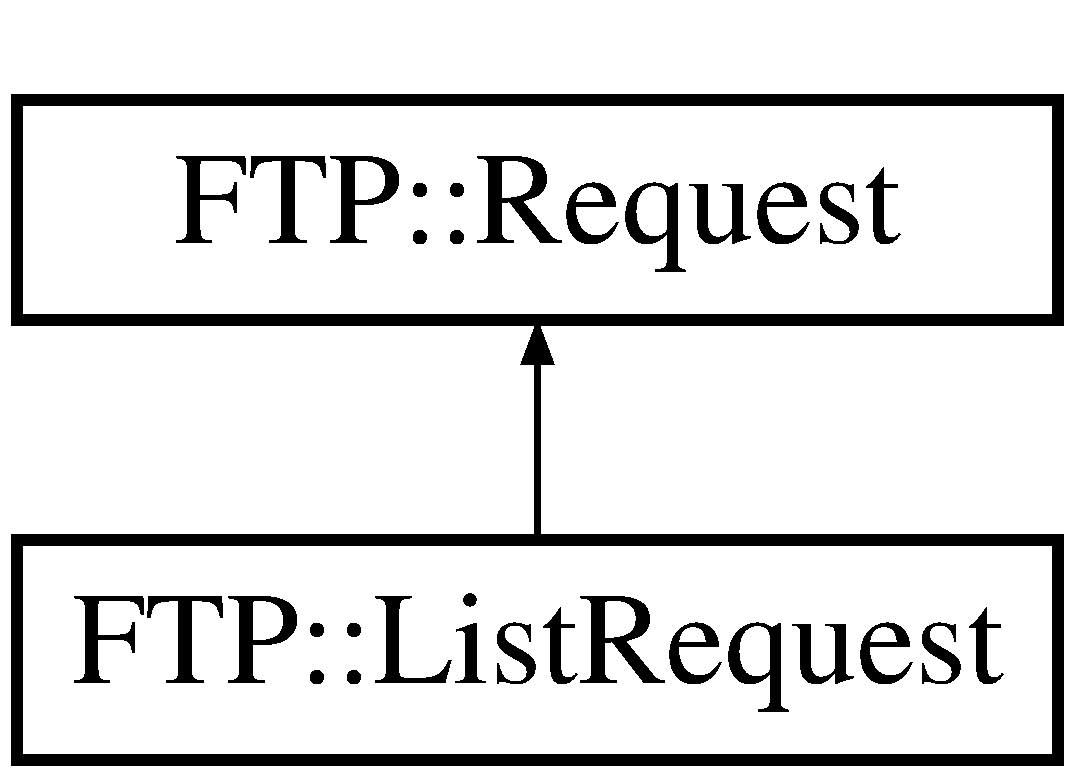
\includegraphics[height=2.000000cm]{classFTP_1_1ListRequest}
\end{center}
\end{figure}
\subsection*{Public Member Functions}
\begin{DoxyCompactItemize}
\item 
\hypertarget{classFTP_1_1ListRequest_aa6b1eb7e03533491a28bf8ba800e1989}{}\hyperlink{classFTP_1_1ListRequest_aa6b1eb7e03533491a28bf8ba800e1989}{List\+Request} ()\label{classFTP_1_1ListRequest_aa6b1eb7e03533491a28bf8ba800e1989}

\begin{DoxyCompactList}\small\item\em \hyperlink{classFTP_1_1ListRequest}{List\+Request} constructor. \end{DoxyCompactList}\end{DoxyCompactItemize}
\subsection*{Static Public Attributes}
\begin{DoxyCompactItemize}
\item 
\hypertarget{classFTP_1_1ListRequest_ac8ac654082b68fbb98934517c0387f67}{}static constexpr const char $\ast$ {\bfseries Command\+Name} = \char`\"{}L\+I\+S\+T\char`\"{}\label{classFTP_1_1ListRequest_ac8ac654082b68fbb98934517c0387f67}

\end{DoxyCompactItemize}


\subsection{Detailed Description}
List request. 

Display every files present in the current directory. 

The documentation for this class was generated from the following file\+:\begin{DoxyCompactItemize}
\item 
C\+:/\+Users/\+Nicolas Cachera/\+Documents/\+Programmation/\+C\+A\+R\+\_\+\+Furet\+T\+P/include/core/message/request/List\+Request.\+h\end{DoxyCompactItemize}

\hypertarget{classFTP_1_1MkdRequest}{}\section{F\+T\+P\+:\+:Mkd\+Request Class Reference}
\label{classFTP_1_1MkdRequest}\index{F\+T\+P\+::\+Mkd\+Request@{F\+T\+P\+::\+Mkd\+Request}}


Mkd request.  




{\ttfamily \#include $<$Mkd\+Request.\+h$>$}

Inheritance diagram for F\+T\+P\+:\+:Mkd\+Request\+:\begin{figure}[H]
\begin{center}
\leavevmode
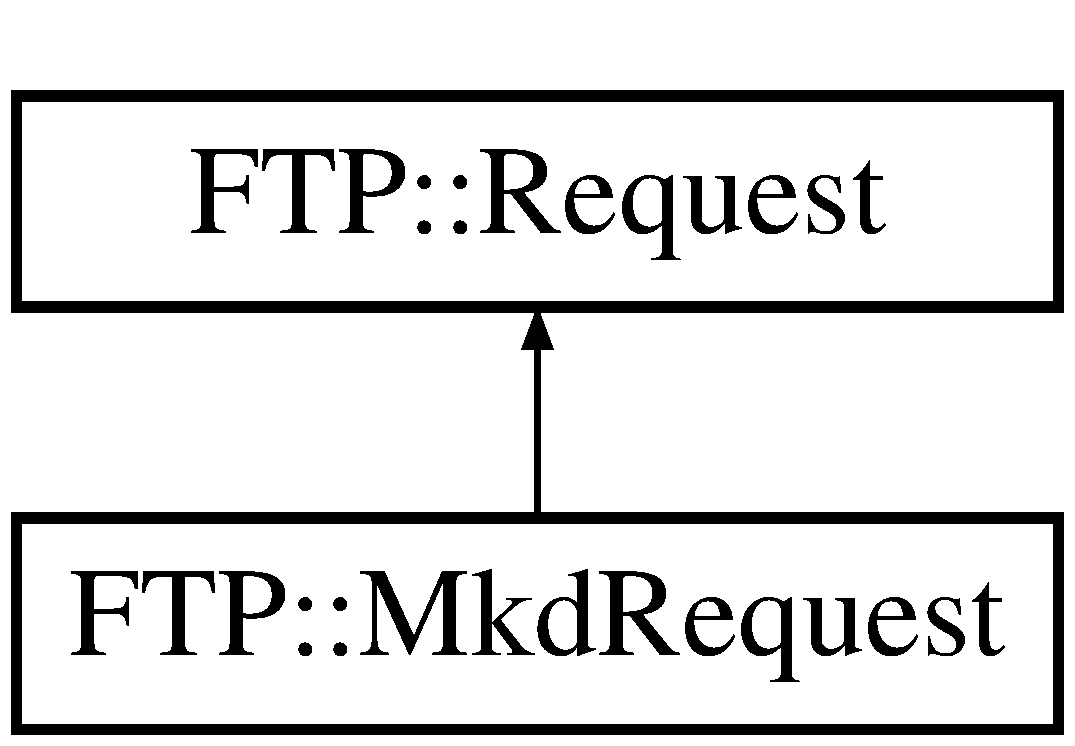
\includegraphics[height=2.000000cm]{classFTP_1_1MkdRequest}
\end{center}
\end{figure}
\subsection*{Public Member Functions}
\begin{DoxyCompactItemize}
\item 
\hyperlink{classFTP_1_1MkdRequest_a1c4565a8d7fbe2bc74ac4db2e2f4d4a9}{Mkd\+Request} (const std\+::string \&name)
\begin{DoxyCompactList}\small\item\em \hyperlink{classFTP_1_1MkdRequest}{Mkd\+Request} constructor. \end{DoxyCompactList}\item 
\hypertarget{classFTP_1_1MkdRequest_ae113af9dc74d782f22f51108186ec388}{}const std\+::string \& {\bfseries get\+Name} () const \label{classFTP_1_1MkdRequest_ae113af9dc74d782f22f51108186ec388}

\end{DoxyCompactItemize}
\subsection*{Static Public Attributes}
\begin{DoxyCompactItemize}
\item 
\hypertarget{classFTP_1_1MkdRequest_a0a5ac61b458cd123dcbbaa97143e2221}{}static constexpr const char $\ast$ {\bfseries Command\+Name} = \char`\"{}M\+K\+D\char`\"{}\label{classFTP_1_1MkdRequest_a0a5ac61b458cd123dcbbaa97143e2221}

\end{DoxyCompactItemize}


\subsection{Detailed Description}
Mkd request. 

Asks the server to create a new folder in the current directory. 

\subsection{Constructor \& Destructor Documentation}
\hypertarget{classFTP_1_1MkdRequest_a1c4565a8d7fbe2bc74ac4db2e2f4d4a9}{}\index{F\+T\+P\+::\+Mkd\+Request@{F\+T\+P\+::\+Mkd\+Request}!Mkd\+Request@{Mkd\+Request}}
\index{Mkd\+Request@{Mkd\+Request}!F\+T\+P\+::\+Mkd\+Request@{F\+T\+P\+::\+Mkd\+Request}}
\subsubsection[{Mkd\+Request}]{\setlength{\rightskip}{0pt plus 5cm}F\+T\+P\+::\+Mkd\+Request\+::\+Mkd\+Request (
\begin{DoxyParamCaption}
\item[{const std\+::string \&}]{name}
\end{DoxyParamCaption}
)}\label{classFTP_1_1MkdRequest_a1c4565a8d7fbe2bc74ac4db2e2f4d4a9}


\hyperlink{classFTP_1_1MkdRequest}{Mkd\+Request} constructor. 


\begin{DoxyParams}{Parameters}
{\em name} & The name of the folder \\
\hline
\end{DoxyParams}


The documentation for this class was generated from the following file\+:\begin{DoxyCompactItemize}
\item 
C\+:/\+Users/\+Nicolas Cachera/\+Documents/\+Programmation/\+C\+A\+R\+\_\+\+Furet\+T\+P/include/core/message/request/Mkd\+Request.\+h\end{DoxyCompactItemize}

\hypertarget{classFTP_1_1NoActiveConnectionException}{}\section{F\+T\+P\+:\+:No\+Active\+Connection\+Exception Class Reference}
\label{classFTP_1_1NoActiveConnectionException}\index{F\+T\+P\+::\+No\+Active\+Connection\+Exception@{F\+T\+P\+::\+No\+Active\+Connection\+Exception}}


\hyperlink{classFTP_1_1Exception}{Exception} launched when there isn\textquotesingle{}t Active connection when it\textquotesingle{}s needed.  




{\ttfamily \#include $<$No\+Active\+Connection\+Exception.\+h$>$}

Inheritance diagram for F\+T\+P\+:\+:No\+Active\+Connection\+Exception\+:\begin{figure}[H]
\begin{center}
\leavevmode
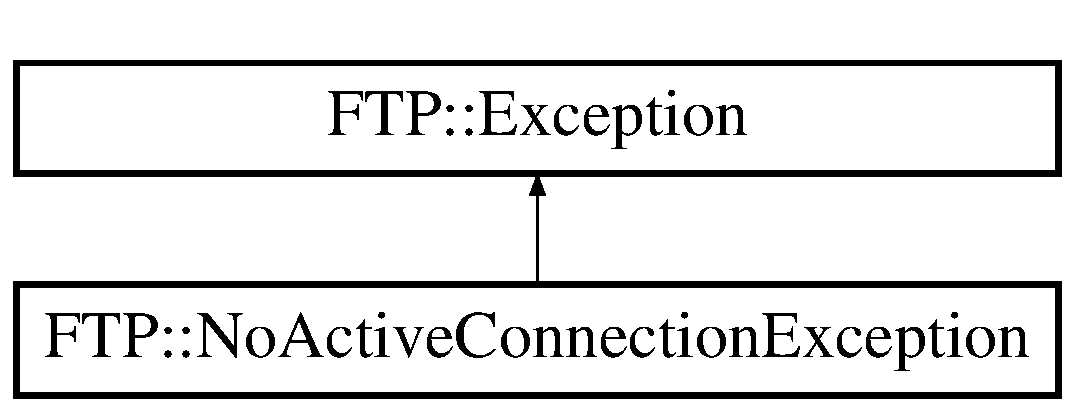
\includegraphics[height=2.000000cm]{classFTP_1_1NoActiveConnectionException}
\end{center}
\end{figure}
\subsection*{Public Member Functions}
\begin{DoxyCompactItemize}
\item 
\hyperlink{classFTP_1_1NoActiveConnectionException_a8ca3caac1e8edfb7b08134935f9b8688}{No\+Active\+Connection\+Exception} (const std\+::string \&message=\char`\"{}\char`\"{})
\begin{DoxyCompactList}\small\item\em \hyperlink{classFTP_1_1NoActiveConnectionException}{No\+Active\+Connection\+Exception} constructor. \end{DoxyCompactList}\end{DoxyCompactItemize}


\subsection{Detailed Description}
\hyperlink{classFTP_1_1Exception}{Exception} launched when there isn\textquotesingle{}t Active connection when it\textquotesingle{}s needed. 

\subsection{Constructor \& Destructor Documentation}
\hypertarget{classFTP_1_1NoActiveConnectionException_a8ca3caac1e8edfb7b08134935f9b8688}{}\index{F\+T\+P\+::\+No\+Active\+Connection\+Exception@{F\+T\+P\+::\+No\+Active\+Connection\+Exception}!No\+Active\+Connection\+Exception@{No\+Active\+Connection\+Exception}}
\index{No\+Active\+Connection\+Exception@{No\+Active\+Connection\+Exception}!F\+T\+P\+::\+No\+Active\+Connection\+Exception@{F\+T\+P\+::\+No\+Active\+Connection\+Exception}}
\subsubsection[{No\+Active\+Connection\+Exception}]{\setlength{\rightskip}{0pt plus 5cm}F\+T\+P\+::\+No\+Active\+Connection\+Exception\+::\+No\+Active\+Connection\+Exception (
\begin{DoxyParamCaption}
\item[{const std\+::string \&}]{message = {\ttfamily \char`\"{}\char`\"{}}}
\end{DoxyParamCaption}
)}\label{classFTP_1_1NoActiveConnectionException_a8ca3caac1e8edfb7b08134935f9b8688}


\hyperlink{classFTP_1_1NoActiveConnectionException}{No\+Active\+Connection\+Exception} constructor. 


\begin{DoxyParams}{Parameters}
{\em message} & A message to print \\
\hline
\end{DoxyParams}


The documentation for this class was generated from the following file\+:\begin{DoxyCompactItemize}
\item 
C\+:/\+Users/\+Nicolas Cachera/\+Documents/\+Programmation/\+C\+A\+R\+\_\+\+Furet\+T\+P/include/exception/No\+Active\+Connection\+Exception.\+h\end{DoxyCompactItemize}

\hypertarget{classFTP_1_1Packet}{}\section{F\+T\+P\+:\+:Packet Class Reference}
\label{classFTP_1_1Packet}\index{F\+T\+P\+::\+Packet@{F\+T\+P\+::\+Packet}}


Class which contains data. \hyperlink{classFTP_1_1Packet}{Packet} are used to send and receive message from sockets.  




{\ttfamily \#include $<$Packet.\+h$>$}

\subsection*{Public Member Functions}
\begin{DoxyCompactItemize}
\item 
\hypertarget{classFTP_1_1Packet_a95e1b1075f22a60bca81da1740533595}{}\hyperlink{classFTP_1_1Packet_a95e1b1075f22a60bca81da1740533595}{Packet} ()\label{classFTP_1_1Packet_a95e1b1075f22a60bca81da1740533595}

\begin{DoxyCompactList}\small\item\em create empty packet \end{DoxyCompactList}\item 
\hypertarget{classFTP_1_1Packet_aa027c8478b3aa7a964a1c5c7a2e57eba}{}\hyperlink{classFTP_1_1Packet_aa027c8478b3aa7a964a1c5c7a2e57eba}{Packet} (const \hyperlink{classFTP_1_1Packet}{Packet} \&that)\label{classFTP_1_1Packet_aa027c8478b3aa7a964a1c5c7a2e57eba}

\begin{DoxyCompactList}\small\item\em create new packet and copy \textquotesingle{}that\textquotesingle{} contents into it \end{DoxyCompactList}\item 
\hypertarget{classFTP_1_1Packet_a0615f4be31088b859d770e6f620e357c}{}\hyperlink{classFTP_1_1Packet_a0615f4be31088b859d770e6f620e357c}{$\sim$\+Packet} ()\label{classFTP_1_1Packet_a0615f4be31088b859d770e6f620e357c}

\begin{DoxyCompactList}\small\item\em destroy packet and free memory \end{DoxyCompactList}\item 
\hypertarget{classFTP_1_1Packet_a896fef76d79779c046dcd1918bc3ee68}{}\hyperlink{classFTP_1_1Packet}{Packet} \& \hyperlink{classFTP_1_1Packet_a896fef76d79779c046dcd1918bc3ee68}{operator=} (const \hyperlink{classFTP_1_1Packet}{Packet} \&that)\label{classFTP_1_1Packet_a896fef76d79779c046dcd1918bc3ee68}

\begin{DoxyCompactList}\small\item\em copy content of another packet into current packet \end{DoxyCompactList}\item 
\hypertarget{classFTP_1_1Packet_ab67e5329d916ca745500c5cc0942a3f1}{}unsigned int {\bfseries get\+Size} () const \label{classFTP_1_1Packet_ab67e5329d916ca745500c5cc0942a3f1}

\item 
\hypertarget{classFTP_1_1Packet_af141e6f529ed3230e562ee3f3340fbcb}{}const char $\ast$ {\bfseries get\+Buffer} () const \label{classFTP_1_1Packet_af141e6f529ed3230e562ee3f3340fbcb}

\item 
\hypertarget{classFTP_1_1Packet_a579ab0ada8b4adbd2685cd6a8389c05a}{}void \hyperlink{classFTP_1_1Packet_a579ab0ada8b4adbd2685cd6a8389c05a}{raw\+Write} (const char $\ast$buffer, unsigned int length)\label{classFTP_1_1Packet_a579ab0ada8b4adbd2685cd6a8389c05a}

\begin{DoxyCompactList}\small\item\em write a raw buffer of size \textquotesingle{}length\textquotesingle{} into the packet \end{DoxyCompactList}\item 
\hypertarget{classFTP_1_1Packet_af3ce1782e8b128d3c5e29cb42ca00f97}{}\hyperlink{classFTP_1_1Packet}{Packet} \& \hyperlink{classFTP_1_1Packet_af3ce1782e8b128d3c5e29cb42ca00f97}{operator$<$$<$} (const std\+::string \&str)\label{classFTP_1_1Packet_af3ce1782e8b128d3c5e29cb42ca00f97}

\begin{DoxyCompactList}\small\item\em write a string at the end of the packet content \end{DoxyCompactList}\item 
\hypertarget{classFTP_1_1Packet_ad8407d95fda0ff5febf2ceb8fdbf67fe}{}\hyperlink{classFTP_1_1Packet}{Packet} \& \hyperlink{classFTP_1_1Packet_ad8407d95fda0ff5febf2ceb8fdbf67fe}{operator$>$$>$} (std\+::string \&str)\label{classFTP_1_1Packet_ad8407d95fda0ff5febf2ceb8fdbf67fe}

\begin{DoxyCompactList}\small\item\em get the next word of the packet content \end{DoxyCompactList}\end{DoxyCompactItemize}
\subsection*{Friends}
\begin{DoxyCompactItemize}
\item 
\hypertarget{classFTP_1_1Packet_a845b2286ebe97771dfb21b69ee0f2f21}{}std\+::ostream \& \hyperlink{classFTP_1_1Packet_a845b2286ebe97771dfb21b69ee0f2f21}{operator$<$$<$} (std\+::ostream \&stream, const \hyperlink{classFTP_1_1Packet}{Packet} \&packet)\label{classFTP_1_1Packet_a845b2286ebe97771dfb21b69ee0f2f21}

\begin{DoxyCompactList}\small\item\em display the content of the packet on the stream \end{DoxyCompactList}\end{DoxyCompactItemize}


\subsection{Detailed Description}
Class which contains data. \hyperlink{classFTP_1_1Packet}{Packet} are used to send and receive message from sockets. 

The documentation for this class was generated from the following file\+:\begin{DoxyCompactItemize}
\item 
C\+:/\+Users/\+Nicolas Cachera/\+Documents/\+Programmation/\+C\+A\+R\+\_\+\+Furet\+T\+P/include/network/Packet.\+h\end{DoxyCompactItemize}

\hypertarget{classFTP_1_1PassRequest}{}\section{F\+T\+P\+:\+:Pass\+Request Class Reference}
\label{classFTP_1_1PassRequest}\index{F\+T\+P\+::\+Pass\+Request@{F\+T\+P\+::\+Pass\+Request}}


Pass request.  




{\ttfamily \#include $<$Pass\+Request.\+h$>$}

Inheritance diagram for F\+T\+P\+:\+:Pass\+Request\+:\begin{figure}[H]
\begin{center}
\leavevmode
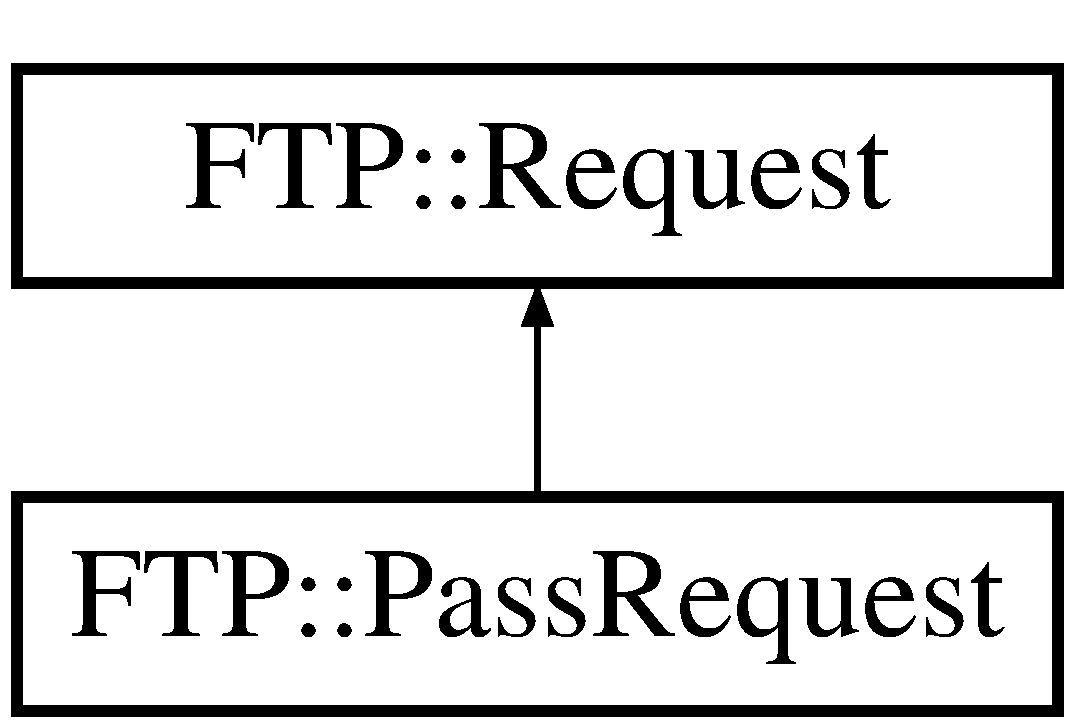
\includegraphics[height=2.000000cm]{classFTP_1_1PassRequest}
\end{center}
\end{figure}
\subsection*{Public Member Functions}
\begin{DoxyCompactItemize}
\item 
\hyperlink{classFTP_1_1PassRequest_a4eb653d4dfd503f9389f5307dd3b802c}{Pass\+Request} (const std\+::string \&password)
\begin{DoxyCompactList}\small\item\em \hyperlink{classFTP_1_1PassRequest}{Pass\+Request} constructor. \end{DoxyCompactList}\item 
\hypertarget{classFTP_1_1PassRequest_a43b1f3a580fc4492cb90713b9a79e537}{}const std\+::string \& {\bfseries get\+Password} () const \label{classFTP_1_1PassRequest_a43b1f3a580fc4492cb90713b9a79e537}

\end{DoxyCompactItemize}
\subsection*{Static Public Attributes}
\begin{DoxyCompactItemize}
\item 
\hypertarget{classFTP_1_1PassRequest_a17183488e2afd35b11bb970f113e7807}{}static constexpr const char $\ast$ {\bfseries Command\+Name} = \char`\"{}P\+A\+S\+S\char`\"{}\label{classFTP_1_1PassRequest_a17183488e2afd35b11bb970f113e7807}

\end{DoxyCompactItemize}


\subsection{Detailed Description}
Pass request. 

\hyperlink{classFTP_1_1Request}{Request} sent to end the login process. Contains the user\textquotesingle{}s password as first argument. 

\subsection{Constructor \& Destructor Documentation}
\hypertarget{classFTP_1_1PassRequest_a4eb653d4dfd503f9389f5307dd3b802c}{}\index{F\+T\+P\+::\+Pass\+Request@{F\+T\+P\+::\+Pass\+Request}!Pass\+Request@{Pass\+Request}}
\index{Pass\+Request@{Pass\+Request}!F\+T\+P\+::\+Pass\+Request@{F\+T\+P\+::\+Pass\+Request}}
\subsubsection[{Pass\+Request}]{\setlength{\rightskip}{0pt plus 5cm}F\+T\+P\+::\+Pass\+Request\+::\+Pass\+Request (
\begin{DoxyParamCaption}
\item[{const std\+::string \&}]{password}
\end{DoxyParamCaption}
)}\label{classFTP_1_1PassRequest_a4eb653d4dfd503f9389f5307dd3b802c}


\hyperlink{classFTP_1_1PassRequest}{Pass\+Request} constructor. 


\begin{DoxyParams}{Parameters}
{\em password} & \hyperlink{structFTP_1_1User}{User}\textquotesingle{}s password \\
\hline
\end{DoxyParams}


The documentation for this class was generated from the following file\+:\begin{DoxyCompactItemize}
\item 
C\+:/\+Users/\+Nicolas Cachera/\+Documents/\+Programmation/\+C\+A\+R\+\_\+\+Furet\+T\+P/include/core/message/request/Pass\+Request.\+h\end{DoxyCompactItemize}

\hypertarget{classFTP_1_1PasvRequest}{}\section{F\+T\+P\+:\+:Pasv\+Request Class Reference}
\label{classFTP_1_1PasvRequest}\index{F\+T\+P\+::\+Pasv\+Request@{F\+T\+P\+::\+Pasv\+Request}}


Pasv request.  




{\ttfamily \#include $<$Pasv\+Request.\+h$>$}

Inheritance diagram for F\+T\+P\+:\+:Pasv\+Request\+:\begin{figure}[H]
\begin{center}
\leavevmode
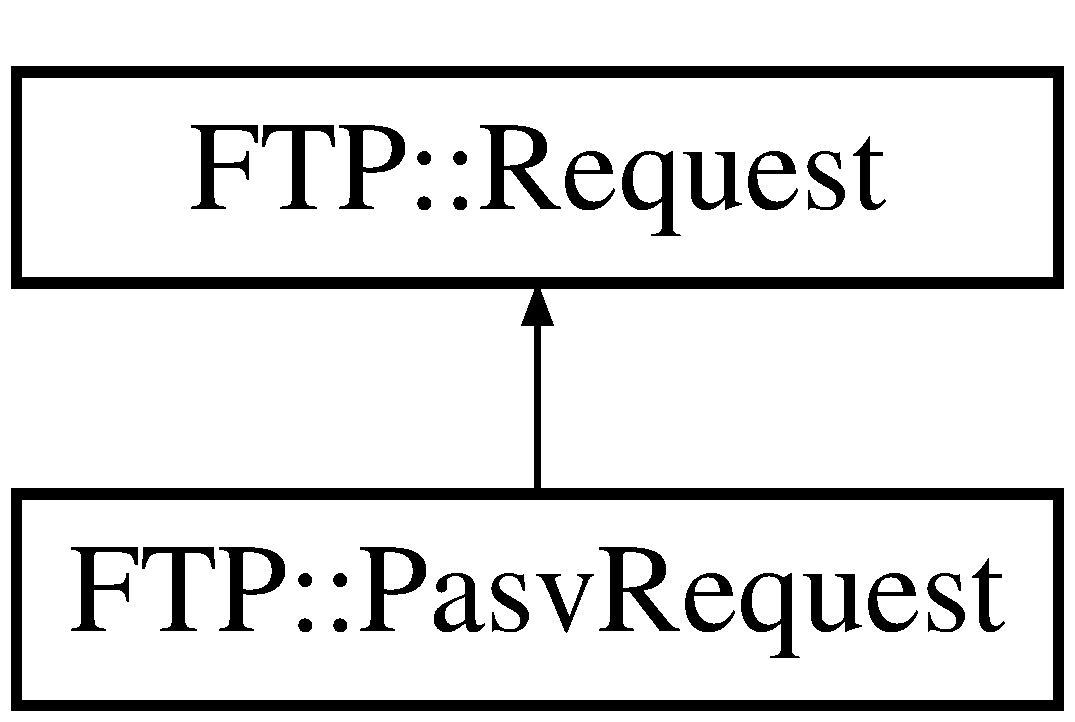
\includegraphics[height=2.000000cm]{classFTP_1_1PasvRequest}
\end{center}
\end{figure}
\subsection*{Public Member Functions}
\begin{DoxyCompactItemize}
\item 
\hypertarget{classFTP_1_1PasvRequest_aa78463de945e73db51aebe44bad1892a}{}\hyperlink{classFTP_1_1PasvRequest_aa78463de945e73db51aebe44bad1892a}{Pasv\+Request} ()\label{classFTP_1_1PasvRequest_aa78463de945e73db51aebe44bad1892a}

\begin{DoxyCompactList}\small\item\em \hyperlink{classFTP_1_1PasvRequest}{Pasv\+Request} constructor. \end{DoxyCompactList}\end{DoxyCompactItemize}
\subsection*{Static Public Attributes}
\begin{DoxyCompactItemize}
\item 
\hypertarget{classFTP_1_1PasvRequest_a0524ca195603ca4bd0e7b33a727373e9}{}static constexpr const char $\ast$ {\bfseries Command\+Name} = \char`\"{}P\+A\+S\+V\char`\"{}\label{classFTP_1_1PasvRequest_a0524ca195603ca4bd0e7b33a727373e9}

\end{DoxyCompactItemize}


\subsection{Detailed Description}
Pasv request. 

\hyperlink{classFTP_1_1Request}{Request} sent in order to enter in passive mode. 

The documentation for this class was generated from the following file\+:\begin{DoxyCompactItemize}
\item 
C\+:/\+Users/\+Nicolas Cachera/\+Documents/\+Programmation/\+C\+A\+R\+\_\+\+Furet\+T\+P/include/core/message/request/Pasv\+Request.\+h\end{DoxyCompactItemize}

\hypertarget{classFTP_1_1PortRequest}{}\section{F\+T\+P\+:\+:Port\+Request Class Reference}
\label{classFTP_1_1PortRequest}\index{F\+T\+P\+::\+Port\+Request@{F\+T\+P\+::\+Port\+Request}}


Port request.  




{\ttfamily \#include $<$Port\+Request.\+h$>$}

Inheritance diagram for F\+T\+P\+:\+:Port\+Request\+:\begin{figure}[H]
\begin{center}
\leavevmode
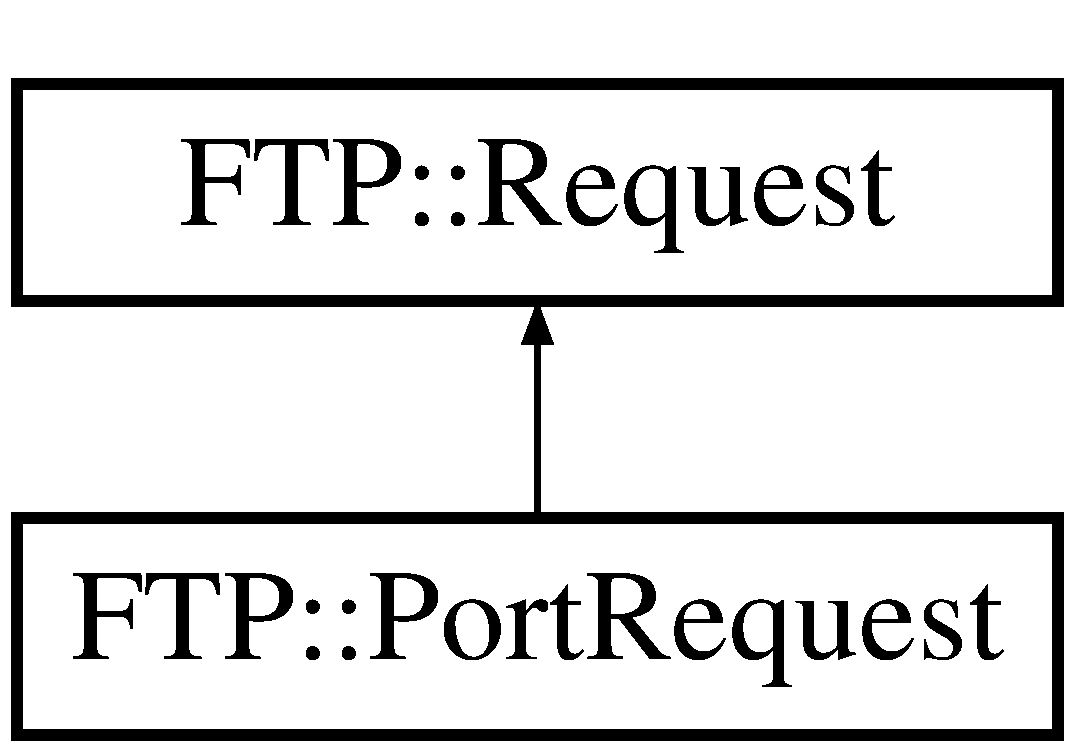
\includegraphics[height=2.000000cm]{classFTP_1_1PortRequest}
\end{center}
\end{figure}
\subsection*{Public Member Functions}
\begin{DoxyCompactItemize}
\item 
\hyperlink{classFTP_1_1PortRequest_a880ff4f41e2bcec2cfac43a6c90c5511}{Port\+Request} (const \hyperlink{classFTP_1_1IP_1_1Address}{I\+P\+::\+Address} \&address, unsigned int port)
\begin{DoxyCompactList}\small\item\em \hyperlink{classFTP_1_1PortRequest}{Port\+Request} constructor. \end{DoxyCompactList}\item 
\hypertarget{classFTP_1_1PortRequest_a056cc2a789af4cf9e2b1655a607803fd}{}const \hyperlink{classFTP_1_1IP_1_1Address}{I\+P\+::\+Address} \& {\bfseries get\+Address} () const \label{classFTP_1_1PortRequest_a056cc2a789af4cf9e2b1655a607803fd}

\item 
\hypertarget{classFTP_1_1PortRequest_a24bba13c833381f9cee9977c838a7571}{}unsigned int {\bfseries get\+Port} () const \label{classFTP_1_1PortRequest_a24bba13c833381f9cee9977c838a7571}

\end{DoxyCompactItemize}
\subsection*{Static Public Attributes}
\begin{DoxyCompactItemize}
\item 
\hypertarget{classFTP_1_1PortRequest_abe4ea52bfb6cce24fb0a0de77d742804}{}static constexpr const char $\ast$ {\bfseries Command\+Name} = \char`\"{}P\+O\+R\+T\char`\"{}\label{classFTP_1_1PortRequest_abe4ea52bfb6cce24fb0a0de77d742804}

\end{DoxyCompactItemize}


\subsection{Detailed Description}
Port request. 

Command sent by the client when he wants to open a new connection. 

\subsection{Constructor \& Destructor Documentation}
\hypertarget{classFTP_1_1PortRequest_a880ff4f41e2bcec2cfac43a6c90c5511}{}\index{F\+T\+P\+::\+Port\+Request@{F\+T\+P\+::\+Port\+Request}!Port\+Request@{Port\+Request}}
\index{Port\+Request@{Port\+Request}!F\+T\+P\+::\+Port\+Request@{F\+T\+P\+::\+Port\+Request}}
\subsubsection[{Port\+Request}]{\setlength{\rightskip}{0pt plus 5cm}F\+T\+P\+::\+Port\+Request\+::\+Port\+Request (
\begin{DoxyParamCaption}
\item[{const {\bf I\+P\+::\+Address} \&}]{address, }
\item[{unsigned int}]{port}
\end{DoxyParamCaption}
)}\label{classFTP_1_1PortRequest_a880ff4f41e2bcec2cfac43a6c90c5511}


\hyperlink{classFTP_1_1PortRequest}{Port\+Request} constructor. 


\begin{DoxyParams}{Parameters}
{\em address} & the new address to connect to \\
\hline
{\em port} & the new port to connect to \\
\hline
\end{DoxyParams}


The documentation for this class was generated from the following file\+:\begin{DoxyCompactItemize}
\item 
C\+:/\+Users/\+Nicolas Cachera/\+Documents/\+Programmation/\+C\+A\+R\+\_\+\+Furet\+T\+P/include/core/message/request/Port\+Request.\+h\end{DoxyCompactItemize}

\hypertarget{classFTP_1_1PwdRequest}{}\section{F\+T\+P\+:\+:Pwd\+Request Class Reference}
\label{classFTP_1_1PwdRequest}\index{F\+T\+P\+::\+Pwd\+Request@{F\+T\+P\+::\+Pwd\+Request}}


Pwd request.  




{\ttfamily \#include $<$Pwd\+Request.\+h$>$}

Inheritance diagram for F\+T\+P\+:\+:Pwd\+Request\+:\begin{figure}[H]
\begin{center}
\leavevmode
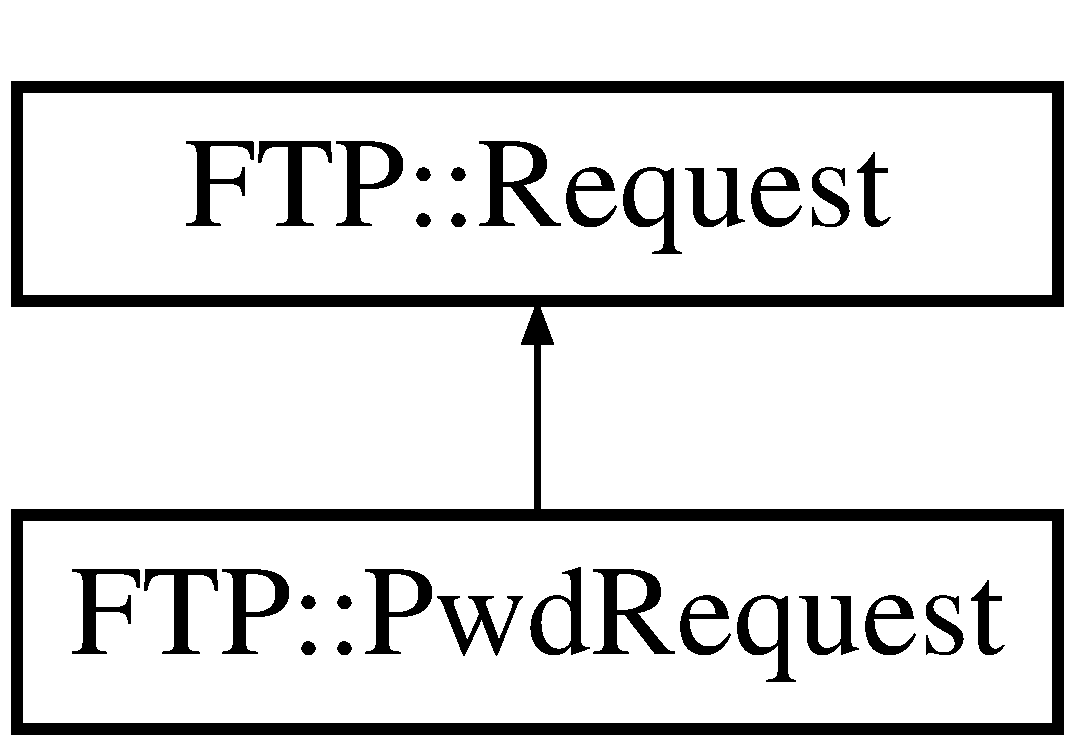
\includegraphics[height=2.000000cm]{classFTP_1_1PwdRequest}
\end{center}
\end{figure}
\subsection*{Public Member Functions}
\begin{DoxyCompactItemize}
\item 
\hypertarget{classFTP_1_1PwdRequest_a403b0aeb6e2ba118c808d16fbe3b78b9}{}\hyperlink{classFTP_1_1PwdRequest_a403b0aeb6e2ba118c808d16fbe3b78b9}{Pwd\+Request} ()\label{classFTP_1_1PwdRequest_a403b0aeb6e2ba118c808d16fbe3b78b9}

\begin{DoxyCompactList}\small\item\em \hyperlink{classFTP_1_1PwdRequest}{Pwd\+Request} constructor. \end{DoxyCompactList}\end{DoxyCompactItemize}
\subsection*{Static Public Attributes}
\begin{DoxyCompactItemize}
\item 
\hypertarget{classFTP_1_1PwdRequest_a5492dc00d110d1c8233af41d0f45c452}{}static constexpr const char $\ast$ {\bfseries Command\+Name} = \char`\"{}P\+W\+D\char`\"{}\label{classFTP_1_1PwdRequest_a5492dc00d110d1c8233af41d0f45c452}

\end{DoxyCompactItemize}


\subsection{Detailed Description}
Pwd request. 

Asks the server to send the current directory pathname. 

The documentation for this class was generated from the following file\+:\begin{DoxyCompactItemize}
\item 
C\+:/\+Users/\+Nicolas Cachera/\+Documents/\+Programmation/\+C\+A\+R\+\_\+\+Furet\+T\+P/include/core/message/request/Pwd\+Request.\+h\end{DoxyCompactItemize}

\hypertarget{classFTP_1_1QuitRequest}{}\section{F\+T\+P\+:\+:Quit\+Request Class Reference}
\label{classFTP_1_1QuitRequest}\index{F\+T\+P\+::\+Quit\+Request@{F\+T\+P\+::\+Quit\+Request}}


Quit request.  




{\ttfamily \#include $<$Quit\+Request.\+h$>$}

Inheritance diagram for F\+T\+P\+:\+:Quit\+Request\+:\begin{figure}[H]
\begin{center}
\leavevmode
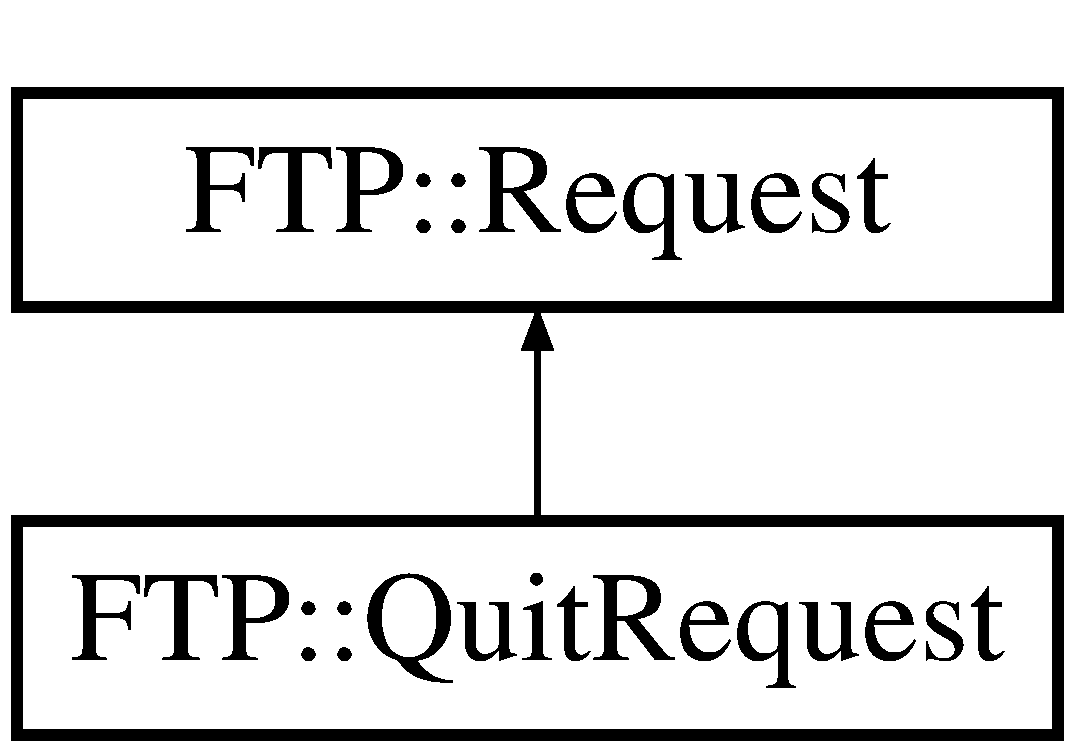
\includegraphics[height=2.000000cm]{classFTP_1_1QuitRequest}
\end{center}
\end{figure}
\subsection*{Public Member Functions}
\begin{DoxyCompactItemize}
\item 
\hypertarget{classFTP_1_1QuitRequest_ac4485b43c00501183cea0eaea01e7349}{}\hyperlink{classFTP_1_1QuitRequest_ac4485b43c00501183cea0eaea01e7349}{Quit\+Request} ()\label{classFTP_1_1QuitRequest_ac4485b43c00501183cea0eaea01e7349}

\begin{DoxyCompactList}\small\item\em \hyperlink{classFTP_1_1QuitRequest}{Quit\+Request} constructor. \end{DoxyCompactList}\end{DoxyCompactItemize}
\subsection*{Static Public Attributes}
\begin{DoxyCompactItemize}
\item 
\hypertarget{classFTP_1_1QuitRequest_ad454c5249faa90ecec425af2ca5a6405}{}static constexpr const char $\ast$ {\bfseries Command\+Name} = \char`\"{}Q\+U\+I\+T\char`\"{}\label{classFTP_1_1QuitRequest_ad454c5249faa90ecec425af2ca5a6405}

\end{DoxyCompactItemize}


\subsection{Detailed Description}
Quit request. 

Command sent to the server when an user quit it. 

The documentation for this class was generated from the following file\+:\begin{DoxyCompactItemize}
\item 
C\+:/\+Users/\+Nicolas Cachera/\+Documents/\+Programmation/\+C\+A\+R\+\_\+\+Furet\+T\+P/include/core/message/request/Quit\+Request.\+h\end{DoxyCompactItemize}

\hypertarget{classFTP_1_1Request}{}\section{F\+T\+P\+:\+:Request Class Reference}
\label{classFTP_1_1Request}\index{F\+T\+P\+::\+Request@{F\+T\+P\+::\+Request}}


Basic request.  




{\ttfamily \#include $<$Request.\+h$>$}

Inheritance diagram for F\+T\+P\+:\+:Request\+:\begin{figure}[H]
\begin{center}
\leavevmode
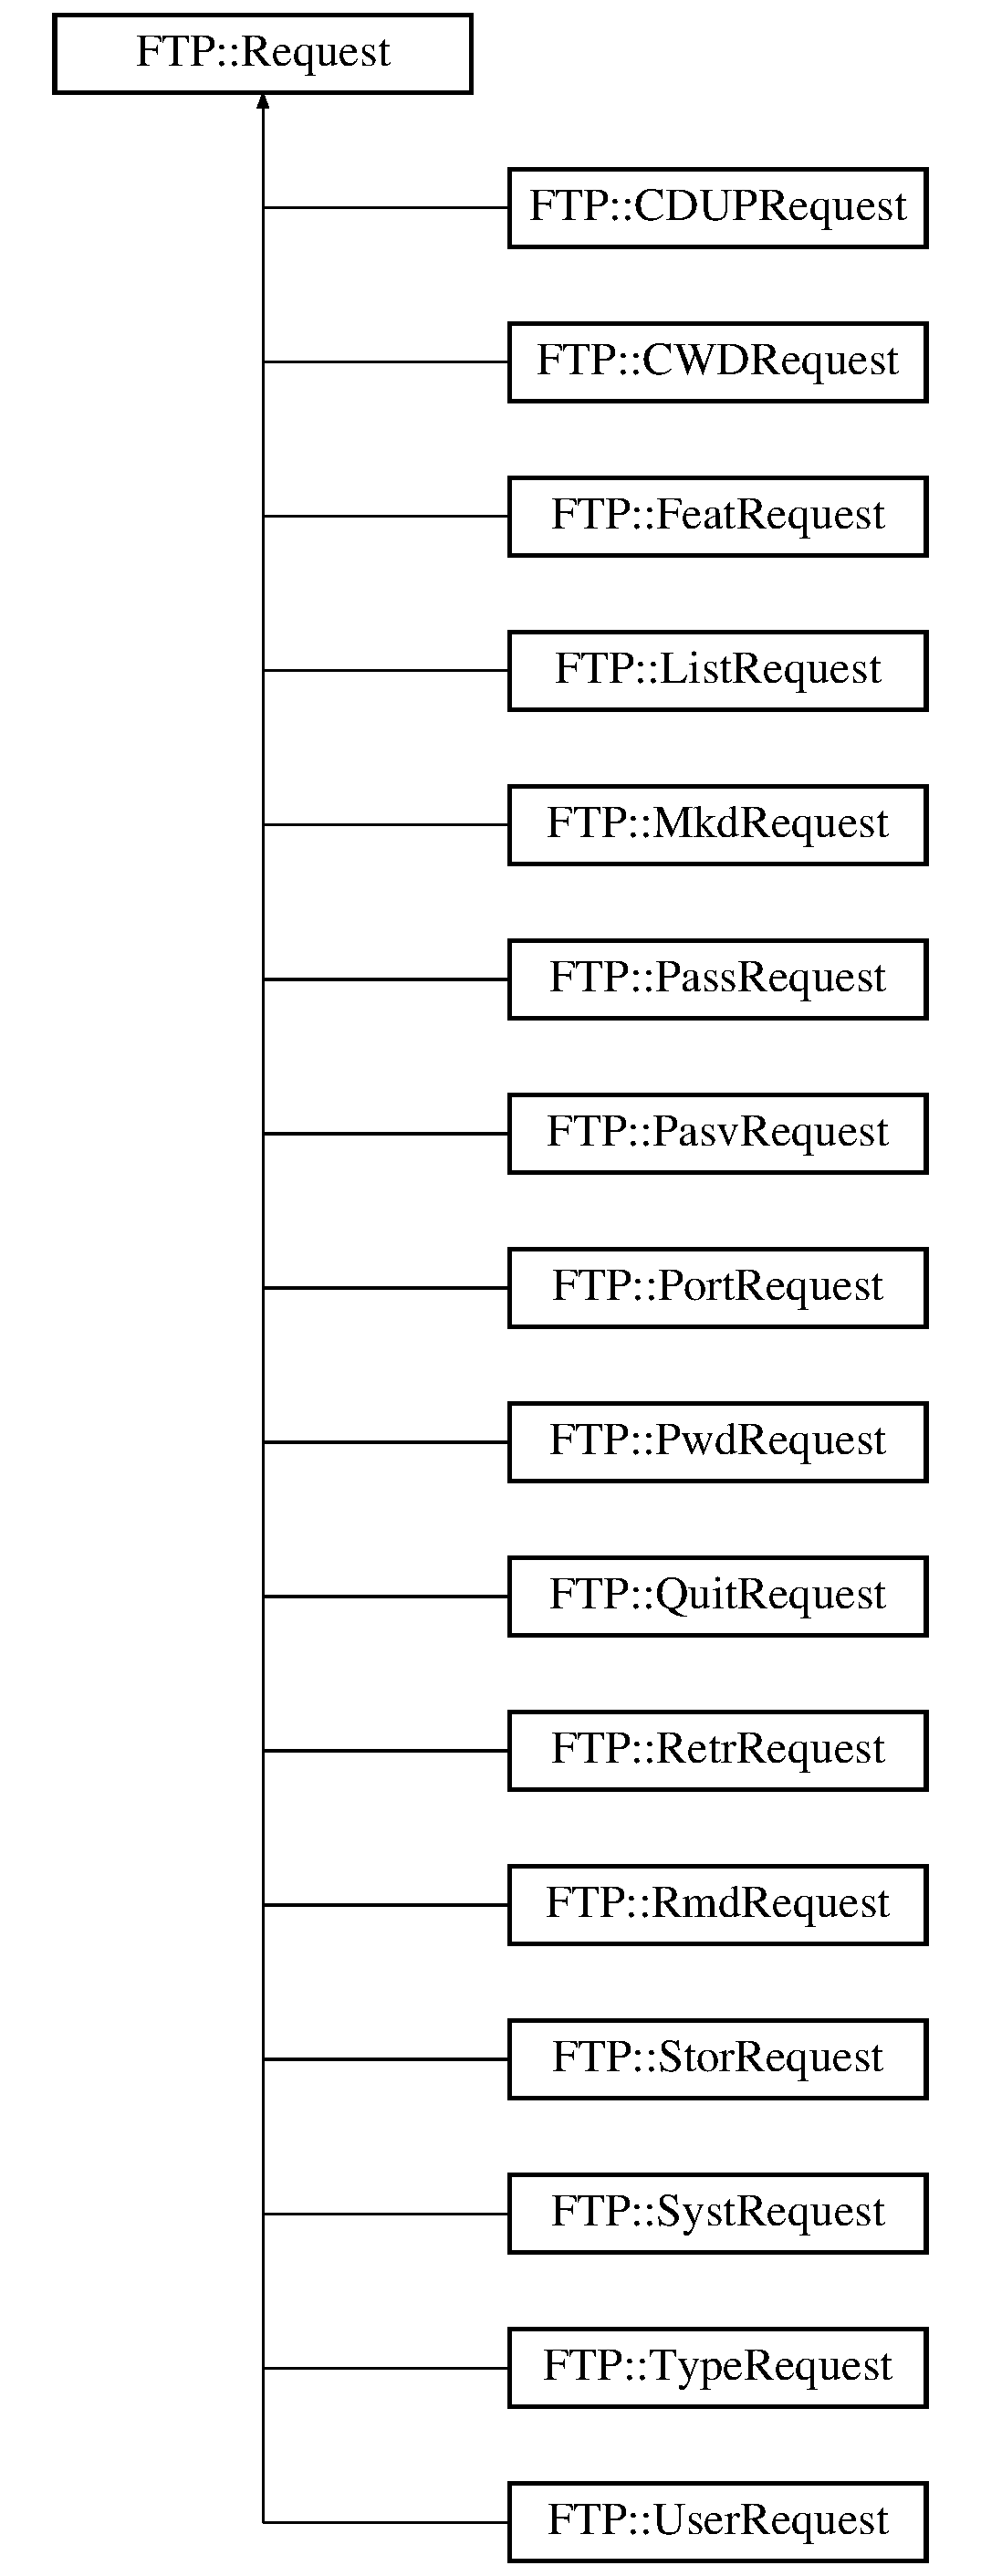
\includegraphics[height=12.000000cm]{classFTP_1_1Request}
\end{center}
\end{figure}
\subsection*{Public Member Functions}
\begin{DoxyCompactItemize}
\item 
\hyperlink{classFTP_1_1Request_a0ac0823bc06e65b29b01c6f260e949c4}{Request} (const std\+::string \&command)
\begin{DoxyCompactList}\small\item\em \hyperlink{classFTP_1_1Request}{Request} constructor. \end{DoxyCompactList}\item 
\hypertarget{classFTP_1_1Request_a450bfde1fc4c9c1f159426b738ffb28a}{}const std\+::string \& {\bfseries get\+Command\+Name} () const \label{classFTP_1_1Request_a450bfde1fc4c9c1f159426b738ffb28a}

\end{DoxyCompactItemize}


\subsection{Detailed Description}
Basic request. 

Represents a packet send by user to the server. 

\subsection{Constructor \& Destructor Documentation}
\hypertarget{classFTP_1_1Request_a0ac0823bc06e65b29b01c6f260e949c4}{}\index{F\+T\+P\+::\+Request@{F\+T\+P\+::\+Request}!Request@{Request}}
\index{Request@{Request}!F\+T\+P\+::\+Request@{F\+T\+P\+::\+Request}}
\subsubsection[{Request}]{\setlength{\rightskip}{0pt plus 5cm}F\+T\+P\+::\+Request\+::\+Request (
\begin{DoxyParamCaption}
\item[{const std\+::string \&}]{command}
\end{DoxyParamCaption}
)}\label{classFTP_1_1Request_a0ac0823bc06e65b29b01c6f260e949c4}


\hyperlink{classFTP_1_1Request}{Request} constructor. 


\begin{DoxyParams}{Parameters}
{\em command} & Command name of the request \\
\hline
\end{DoxyParams}


The documentation for this class was generated from the following file\+:\begin{DoxyCompactItemize}
\item 
C\+:/\+Users/\+Nicolas Cachera/\+Documents/\+Programmation/\+C\+A\+R\+\_\+\+Furet\+T\+P/include/core/message/request/Request.\+h\end{DoxyCompactItemize}

\hypertarget{classFTP_1_1RequestFactory}{}\section{F\+T\+P\+:\+:Request\+Factory Class Reference}
\label{classFTP_1_1RequestFactory}\index{F\+T\+P\+::\+Request\+Factory@{F\+T\+P\+::\+Request\+Factory}}


Determine the class of request packet.  




{\ttfamily \#include $<$Request\+Factory.\+h$>$}

\subsection*{Static Public Member Functions}
\begin{DoxyCompactItemize}
\item 
static \hyperlink{classFTP_1_1Request}{Request} $\ast$ \hyperlink{classFTP_1_1RequestFactory_ac53c72a15f6f91db30d6b0dfa11425dc}{eval} (\hyperlink{classFTP_1_1Packet}{Packet} \&packet)
\begin{DoxyCompactList}\small\item\em Create a request from the packet. \end{DoxyCompactList}\end{DoxyCompactItemize}


\subsection{Detailed Description}
Determine the class of request packet. 

\hyperlink{classFTP_1_1RequestFactory}{Request\+Factory} is a static class. It evaluate a packet in order to create a request from it. 

\subsection{Member Function Documentation}
\hypertarget{classFTP_1_1RequestFactory_ac53c72a15f6f91db30d6b0dfa11425dc}{}\index{F\+T\+P\+::\+Request\+Factory@{F\+T\+P\+::\+Request\+Factory}!eval@{eval}}
\index{eval@{eval}!F\+T\+P\+::\+Request\+Factory@{F\+T\+P\+::\+Request\+Factory}}
\subsubsection[{eval}]{\setlength{\rightskip}{0pt plus 5cm}static {\bf Request}$\ast$ F\+T\+P\+::\+Request\+Factory\+::eval (
\begin{DoxyParamCaption}
\item[{{\bf Packet} \&}]{packet}
\end{DoxyParamCaption}
)\hspace{0.3cm}{\ttfamily [static]}}\label{classFTP_1_1RequestFactory_ac53c72a15f6f91db30d6b0dfa11425dc}


Create a request from the packet. 


\begin{DoxyParams}{Parameters}
{\em packet} & The packet to evaluate \\
\hline
\end{DoxyParams}
\begin{DoxyReturn}{Returns}
F\+T\+P\+Message
\end{DoxyReturn}
The receiver is responsible of the returned object deletion 

The documentation for this class was generated from the following file\+:\begin{DoxyCompactItemize}
\item 
C\+:/\+Users/\+Nicolas Cachera/\+Documents/\+Programmation/\+C\+A\+R\+\_\+\+Furet\+T\+P/include/core/message/request/Request\+Factory.\+h\end{DoxyCompactItemize}

\hypertarget{classFTP_1_1RequestHandler}{}\section{F\+T\+P\+:\+:Request\+Handler Class Reference}
\label{classFTP_1_1RequestHandler}\index{F\+T\+P\+::\+Request\+Handler@{F\+T\+P\+::\+Request\+Handler}}


Interpret and execute a known request.  




{\ttfamily \#include $<$Request\+Handler.\+h$>$}

\subsection*{Static Public Member Functions}
\begin{DoxyCompactItemize}
\item 
static void \hyperlink{classFTP_1_1RequestHandler_a200aabd95bfbc5ff6c32d37e585d6310}{process} (\hyperlink{classFTP_1_1Request}{Request} \&request, \hyperlink{classFTP_1_1Client}{Client} $\ast$client)
\begin{DoxyCompactList}\small\item\em Call the right request handler for the request. \end{DoxyCompactList}\end{DoxyCompactItemize}


\subsection{Detailed Description}
Interpret and execute a known request. 

\hyperlink{classFTP_1_1RequestHandler}{Request\+Handler} is a static Class. It receives a request on its process method and then call the right method to execute it. 

\subsection{Member Function Documentation}
\hypertarget{classFTP_1_1RequestHandler_a200aabd95bfbc5ff6c32d37e585d6310}{}\index{F\+T\+P\+::\+Request\+Handler@{F\+T\+P\+::\+Request\+Handler}!process@{process}}
\index{process@{process}!F\+T\+P\+::\+Request\+Handler@{F\+T\+P\+::\+Request\+Handler}}
\subsubsection[{process}]{\setlength{\rightskip}{0pt plus 5cm}static void F\+T\+P\+::\+Request\+Handler\+::process (
\begin{DoxyParamCaption}
\item[{{\bf Request} \&}]{request, }
\item[{{\bf Client} $\ast$}]{client}
\end{DoxyParamCaption}
)\hspace{0.3cm}{\ttfamily [static]}}\label{classFTP_1_1RequestHandler_a200aabd95bfbc5ff6c32d37e585d6310}


Call the right request handler for the request. 


\begin{DoxyParams}{Parameters}
{\em request} & \hyperlink{classFTP_1_1Request}{Request} to interpret and execute \\
\hline
{\em client} & the user who sends the request \\
\hline
\end{DoxyParams}


The documentation for this class was generated from the following file\+:\begin{DoxyCompactItemize}
\item 
C\+:/\+Users/\+Nicolas Cachera/\+Documents/\+Programmation/\+C\+A\+R\+\_\+\+Furet\+T\+P/include/core/Request\+Handler.\+h\end{DoxyCompactItemize}

\hypertarget{classFTP_1_1RetrRequest}{}\section{F\+T\+P\+:\+:Retr\+Request Class Reference}
\label{classFTP_1_1RetrRequest}\index{F\+T\+P\+::\+Retr\+Request@{F\+T\+P\+::\+Retr\+Request}}


Retr request.  




{\ttfamily \#include $<$Retr\+Request.\+h$>$}

Inheritance diagram for F\+T\+P\+:\+:Retr\+Request\+:\begin{figure}[H]
\begin{center}
\leavevmode
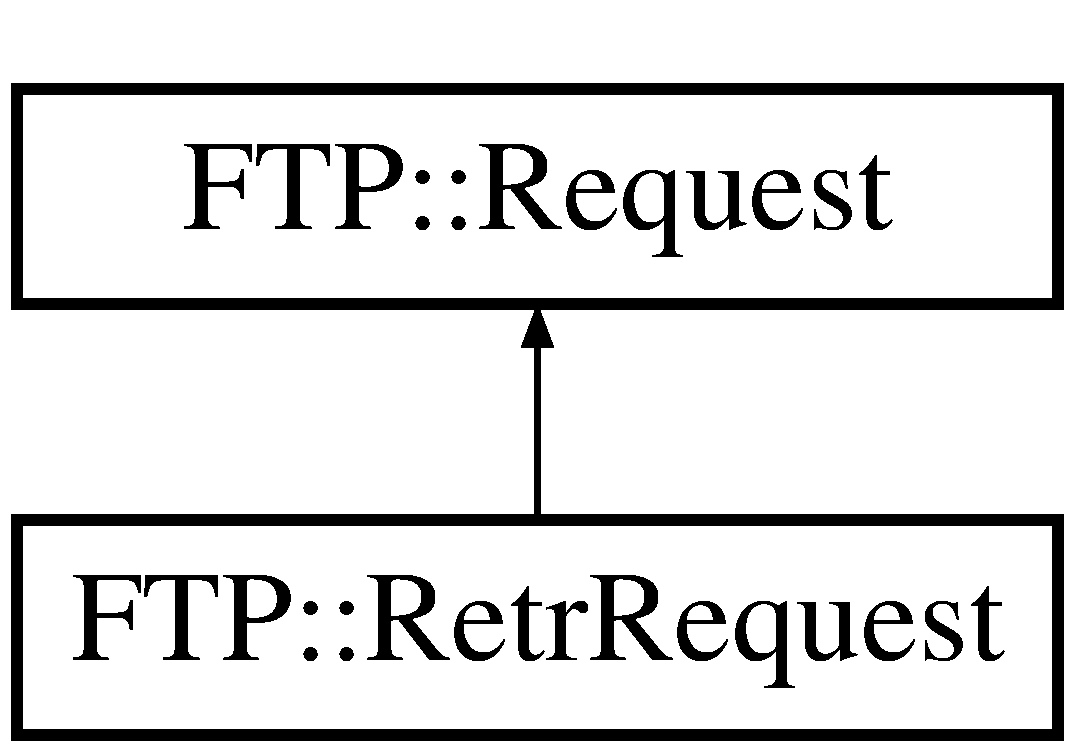
\includegraphics[height=2.000000cm]{classFTP_1_1RetrRequest}
\end{center}
\end{figure}
\subsection*{Public Member Functions}
\begin{DoxyCompactItemize}
\item 
\hyperlink{classFTP_1_1RetrRequest_a97bf717da1cf5ef47cd08d09db7fcb77}{Retr\+Request} (const std\+::string \&filename)
\begin{DoxyCompactList}\small\item\em \hyperlink{classFTP_1_1RetrRequest}{Retr\+Request} constructor. \end{DoxyCompactList}\item 
\hypertarget{classFTP_1_1RetrRequest_a3c558dccb6b1efac1138e31c4957c524}{}const std\+::string \& {\bfseries get\+Filename} () const \label{classFTP_1_1RetrRequest_a3c558dccb6b1efac1138e31c4957c524}

\end{DoxyCompactItemize}
\subsection*{Static Public Attributes}
\begin{DoxyCompactItemize}
\item 
\hypertarget{classFTP_1_1RetrRequest_ad28da02570e40fac7f7ae3136b71acdf}{}static constexpr const char $\ast$ {\bfseries Command\+Name} = \char`\"{}R\+E\+T\+R\char`\"{}\label{classFTP_1_1RetrRequest_ad28da02570e40fac7f7ae3136b71acdf}

\end{DoxyCompactItemize}


\subsection{Detailed Description}
Retr request. 

Command sent by the client to receive a remote file. 

\subsection{Constructor \& Destructor Documentation}
\hypertarget{classFTP_1_1RetrRequest_a97bf717da1cf5ef47cd08d09db7fcb77}{}\index{F\+T\+P\+::\+Retr\+Request@{F\+T\+P\+::\+Retr\+Request}!Retr\+Request@{Retr\+Request}}
\index{Retr\+Request@{Retr\+Request}!F\+T\+P\+::\+Retr\+Request@{F\+T\+P\+::\+Retr\+Request}}
\subsubsection[{Retr\+Request}]{\setlength{\rightskip}{0pt plus 5cm}F\+T\+P\+::\+Retr\+Request\+::\+Retr\+Request (
\begin{DoxyParamCaption}
\item[{const std\+::string \&}]{filename}
\end{DoxyParamCaption}
)}\label{classFTP_1_1RetrRequest_a97bf717da1cf5ef47cd08d09db7fcb77}


\hyperlink{classFTP_1_1RetrRequest}{Retr\+Request} constructor. 


\begin{DoxyParams}{Parameters}
{\em filename} & The file to receive \\
\hline
\end{DoxyParams}


The documentation for this class was generated from the following file\+:\begin{DoxyCompactItemize}
\item 
C\+:/\+Users/\+Nicolas Cachera/\+Documents/\+Programmation/\+C\+A\+R\+\_\+\+Furet\+T\+P/include/core/message/request/Retr\+Request.\+h\end{DoxyCompactItemize}

\hypertarget{classFTP_1_1RmdRequest}{}\section{F\+T\+P\+:\+:Rmd\+Request Class Reference}
\label{classFTP_1_1RmdRequest}\index{F\+T\+P\+::\+Rmd\+Request@{F\+T\+P\+::\+Rmd\+Request}}


Rmd request.  




{\ttfamily \#include $<$Rmd\+Request.\+h$>$}

Inheritance diagram for F\+T\+P\+:\+:Rmd\+Request\+:\begin{figure}[H]
\begin{center}
\leavevmode
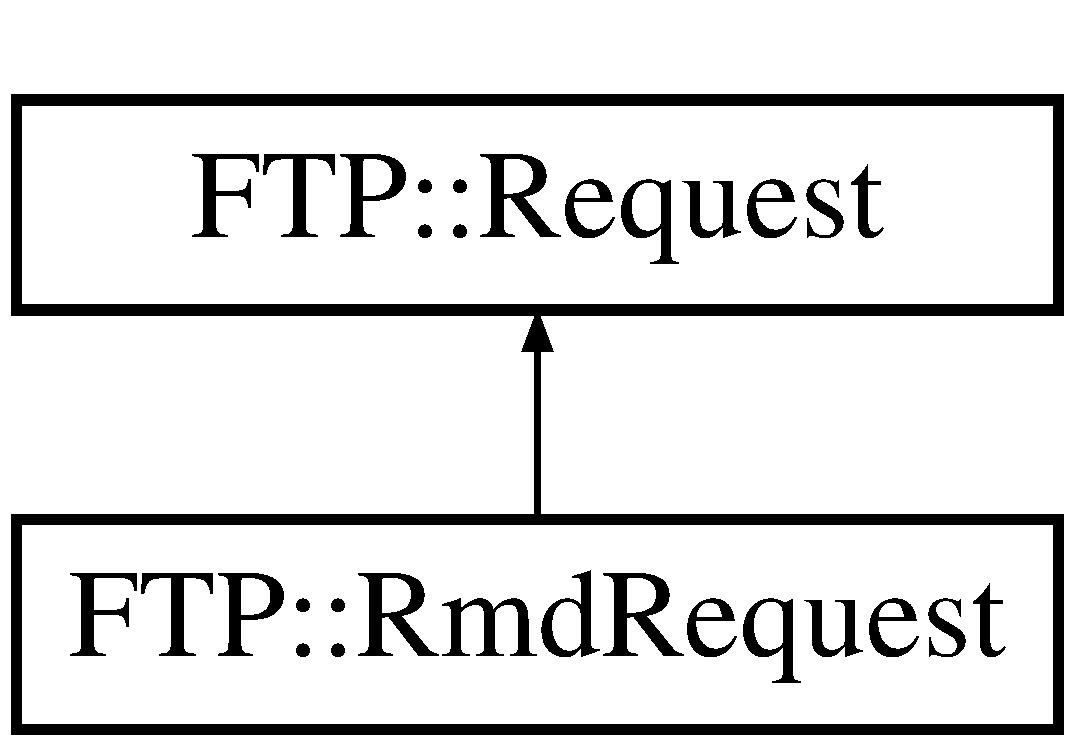
\includegraphics[height=2.000000cm]{classFTP_1_1RmdRequest}
\end{center}
\end{figure}
\subsection*{Public Member Functions}
\begin{DoxyCompactItemize}
\item 
\hyperlink{classFTP_1_1RmdRequest_a3448c5596eaa91cecc3f28ed11daff21}{Rmd\+Request} (const std\+::string \&name)
\begin{DoxyCompactList}\small\item\em \hyperlink{classFTP_1_1RmdRequest}{Rmd\+Request} constructor. \end{DoxyCompactList}\item 
\hypertarget{classFTP_1_1RmdRequest_a35c6a64e5187959710215f04598a6320}{}const std\+::string \& {\bfseries get\+Name} () const \label{classFTP_1_1RmdRequest_a35c6a64e5187959710215f04598a6320}

\end{DoxyCompactItemize}
\subsection*{Static Public Attributes}
\begin{DoxyCompactItemize}
\item 
\hypertarget{classFTP_1_1RmdRequest_ae3771e8e3f539659d04cd4219ad09930}{}static constexpr const char $\ast$ {\bfseries Command\+Name} = \char`\"{}R\+M\+D\char`\"{}\label{classFTP_1_1RmdRequest_ae3771e8e3f539659d04cd4219ad09930}

\end{DoxyCompactItemize}


\subsection{Detailed Description}
Rmd request. 

Asks the server to delete a folder in the current directory. 

\subsection{Constructor \& Destructor Documentation}
\hypertarget{classFTP_1_1RmdRequest_a3448c5596eaa91cecc3f28ed11daff21}{}\index{F\+T\+P\+::\+Rmd\+Request@{F\+T\+P\+::\+Rmd\+Request}!Rmd\+Request@{Rmd\+Request}}
\index{Rmd\+Request@{Rmd\+Request}!F\+T\+P\+::\+Rmd\+Request@{F\+T\+P\+::\+Rmd\+Request}}
\subsubsection[{Rmd\+Request}]{\setlength{\rightskip}{0pt plus 5cm}F\+T\+P\+::\+Rmd\+Request\+::\+Rmd\+Request (
\begin{DoxyParamCaption}
\item[{const std\+::string \&}]{name}
\end{DoxyParamCaption}
)}\label{classFTP_1_1RmdRequest_a3448c5596eaa91cecc3f28ed11daff21}


\hyperlink{classFTP_1_1RmdRequest}{Rmd\+Request} constructor. 


\begin{DoxyParams}{Parameters}
{\em name} & The name of the folder to delete. \\
\hline
\end{DoxyParams}


The documentation for this class was generated from the following file\+:\begin{DoxyCompactItemize}
\item 
C\+:/\+Users/\+Nicolas Cachera/\+Documents/\+Programmation/\+C\+A\+R\+\_\+\+Furet\+T\+P/include/core/message/request/Rmd\+Request.\+h\end{DoxyCompactItemize}

\hypertarget{classFTP_1_1ServerConfiguration}{}\section{F\+T\+P\+:\+:Server\+Configuration Class Reference}
\label{classFTP_1_1ServerConfiguration}\index{F\+T\+P\+::\+Server\+Configuration@{F\+T\+P\+::\+Server\+Configuration}}


Current configuration of the server.  




{\ttfamily \#include $<$Server\+Configuration.\+h$>$}

\subsection*{Public Member Functions}
\begin{DoxyCompactItemize}
\item 
\hypertarget{classFTP_1_1ServerConfiguration_a3bd14902cfa646699d2d782d95de673a}{}\hyperlink{classFTP_1_1ServerConfiguration_a3bd14902cfa646699d2d782d95de673a}{Server\+Configuration} ()\label{classFTP_1_1ServerConfiguration_a3bd14902cfa646699d2d782d95de673a}

\begin{DoxyCompactList}\small\item\em \hyperlink{classFTP_1_1ServerConfiguration}{Server\+Configuration} constructor. \end{DoxyCompactList}\item 
\hypertarget{classFTP_1_1ServerConfiguration_a11b98a6266117f6a3e18640dbd532c2b}{}void \hyperlink{classFTP_1_1ServerConfiguration_a11b98a6266117f6a3e18640dbd532c2b}{load\+Default} ()\label{classFTP_1_1ServerConfiguration_a11b98a6266117f6a3e18640dbd532c2b}

\begin{DoxyCompactList}\small\item\em Load the default server configuration. \end{DoxyCompactList}\item 
\hypertarget{classFTP_1_1ServerConfiguration_aef31c0113abb25ab40875212fda7172e}{}\hyperlink{classFTP_1_1UserList}{User\+List} \& {\bfseries get\+User\+List} ()\label{classFTP_1_1ServerConfiguration_aef31c0113abb25ab40875212fda7172e}

\item 
\hypertarget{classFTP_1_1ServerConfiguration_a08aced6da32db6cdc904f5a8292869d7}{}const \hyperlink{classFTP_1_1UserList}{User\+List} \& {\bfseries get\+User\+List} () const \label{classFTP_1_1ServerConfiguration_a08aced6da32db6cdc904f5a8292869d7}

\item 
\hypertarget{classFTP_1_1ServerConfiguration_ac1247c63b4e2501931137f3d2093a94f}{}const std\+::string \& {\bfseries get\+User\+Configuration\+Pathname} () const \label{classFTP_1_1ServerConfiguration_ac1247c63b4e2501931137f3d2093a94f}

\item 
\hypertarget{classFTP_1_1ServerConfiguration_a511395794c7c6ec3d14241ae46089891}{}unsigned int {\bfseries get\+Bind\+Port} () const \label{classFTP_1_1ServerConfiguration_a511395794c7c6ec3d14241ae46089891}

\item 
\hypertarget{classFTP_1_1ServerConfiguration_a6a943d6b2299fcc9e335ae8afad8a565}{}const std\+::string \& {\bfseries get\+M\+O\+T\+D} () const \label{classFTP_1_1ServerConfiguration_a6a943d6b2299fcc9e335ae8afad8a565}

\item 
\hypertarget{classFTP_1_1ServerConfiguration_a4fc696bd9844369a9c494b4df1d6e87e}{}void {\bfseries set\+Bind\+Port} (unsigned int port)\label{classFTP_1_1ServerConfiguration_a4fc696bd9844369a9c494b4df1d6e87e}

\end{DoxyCompactItemize}


\subsection{Detailed Description}
Current configuration of the server. 

Contains user\textquotesingle{}s account informations, communication port and message of the day 

The documentation for this class was generated from the following file\+:\begin{DoxyCompactItemize}
\item 
C\+:/\+Users/\+Nicolas Cachera/\+Documents/\+Programmation/\+C\+A\+R\+\_\+\+Furet\+T\+P/include/core/Server\+Configuration.\+h\end{DoxyCompactItemize}

\hypertarget{classFTP_1_1TCP_1_1Socket}{}\section{F\+T\+P\+:\+:T\+C\+P\+:\+:Socket Class Reference}
\label{classFTP_1_1TCP_1_1Socket}\index{F\+T\+P\+::\+T\+C\+P\+::\+Socket@{F\+T\+P\+::\+T\+C\+P\+::\+Socket}}
\subsection*{Public Member Functions}
\begin{DoxyCompactItemize}
\item 
\hypertarget{classFTP_1_1TCP_1_1Socket_a38968f94a259b3052b4aada84ed7bcca}{}\hyperlink{classFTP_1_1TCP_1_1Socket_a38968f94a259b3052b4aada84ed7bcca}{Socket} ()\label{classFTP_1_1TCP_1_1Socket_a38968f94a259b3052b4aada84ed7bcca}

\begin{DoxyCompactList}\small\item\em create on non connected socket \end{DoxyCompactList}\item 
\hypertarget{classFTP_1_1TCP_1_1Socket_a13f3818892ac508f3240ca55db98459b}{}\hyperlink{classFTP_1_1TCP_1_1Socket_a13f3818892ac508f3240ca55db98459b}{Socket} (\hyperlink{classFTP_1_1TCP_1_1Socket}{Socket} \&\&that)\label{classFTP_1_1TCP_1_1Socket_a13f3818892ac508f3240ca55db98459b}

\begin{DoxyCompactList}\small\item\em move the socket from \textquotesingle{}that\textquotesingle{} \end{DoxyCompactList}\item 
\hypertarget{classFTP_1_1TCP_1_1Socket_a17e008f492188ab6f9114ff68b0c160b}{}\hyperlink{classFTP_1_1TCP_1_1Socket_a17e008f492188ab6f9114ff68b0c160b}{$\sim$\+Socket} ()\label{classFTP_1_1TCP_1_1Socket_a17e008f492188ab6f9114ff68b0c160b}

\begin{DoxyCompactList}\small\item\em destroy socket and close it connection if he is connected \end{DoxyCompactList}\item 
void \hyperlink{classFTP_1_1TCP_1_1Socket_a220e0105754cdf9378411b24809a4f04}{connect} (const \hyperlink{classFTP_1_1IP_1_1Address}{I\+P\+::\+Address} \&address, unsigned int port)
\begin{DoxyCompactList}\small\item\em connect the socket to the target \textquotesingle{}address\textquotesingle{} \+: \textquotesingle{}port\textquotesingle{} socket \end{DoxyCompactList}\item 
void \hyperlink{classFTP_1_1TCP_1_1Socket_a1a06bb837f2a2d82f3477ecf4da373c7}{receive} (\hyperlink{classFTP_1_1Packet}{Packet} \&packet)
\begin{DoxyCompactList}\small\item\em wait and receive a packet and transfere it content into \textquotesingle{}packet\textquotesingle{} \end{DoxyCompactList}\item 
void \hyperlink{classFTP_1_1TCP_1_1Socket_a7ebcedc1c8baba1a838bdb46babea2eb}{send} (const \hyperlink{classFTP_1_1Packet}{Packet} \&packet)
\begin{DoxyCompactList}\small\item\em send a packet with the content of \textquotesingle{}packet\textquotesingle{} \end{DoxyCompactList}\item 
\hypertarget{classFTP_1_1TCP_1_1Socket_a783815d519b4f76ac7f25e946e8be21e}{}void \hyperlink{classFTP_1_1TCP_1_1Socket_a783815d519b4f76ac7f25e946e8be21e}{close} ()\label{classFTP_1_1TCP_1_1Socket_a783815d519b4f76ac7f25e946e8be21e}

\begin{DoxyCompactList}\small\item\em close the socket connection \end{DoxyCompactList}\item 
\hypertarget{classFTP_1_1TCP_1_1Socket_a9323b1947771c55468a303199742a840}{}bool \hyperlink{classFTP_1_1TCP_1_1Socket_a9323b1947771c55468a303199742a840}{is\+Open} () const \label{classFTP_1_1TCP_1_1Socket_a9323b1947771c55468a303199742a840}

\begin{DoxyCompactList}\small\item\em return true if the socket is currently connected with another socket, false otherwhise \end{DoxyCompactList}\item 
\hypertarget{classFTP_1_1TCP_1_1Socket_a79f3892a2088f566286baf5e4e89f939}{}const \hyperlink{classFTP_1_1IP_1_1Address}{I\+P\+::\+Address} \& {\bfseries get\+Address} () const \label{classFTP_1_1TCP_1_1Socket_a79f3892a2088f566286baf5e4e89f939}

\end{DoxyCompactItemize}
\subsection*{Friends}
\begin{DoxyCompactItemize}
\item 
\hypertarget{classFTP_1_1TCP_1_1Socket_a53a20affc0dd32b432b7e596a68002fe}{}class {\bfseries Listener}\label{classFTP_1_1TCP_1_1Socket_a53a20affc0dd32b432b7e596a68002fe}

\end{DoxyCompactItemize}


\subsection{Member Function Documentation}
\hypertarget{classFTP_1_1TCP_1_1Socket_a220e0105754cdf9378411b24809a4f04}{}\index{F\+T\+P\+::\+T\+C\+P\+::\+Socket@{F\+T\+P\+::\+T\+C\+P\+::\+Socket}!connect@{connect}}
\index{connect@{connect}!F\+T\+P\+::\+T\+C\+P\+::\+Socket@{F\+T\+P\+::\+T\+C\+P\+::\+Socket}}
\subsubsection[{connect}]{\setlength{\rightskip}{0pt plus 5cm}void F\+T\+P\+::\+T\+C\+P\+::\+Socket\+::connect (
\begin{DoxyParamCaption}
\item[{const {\bf I\+P\+::\+Address} \&}]{address, }
\item[{unsigned int}]{port}
\end{DoxyParamCaption}
)}\label{classFTP_1_1TCP_1_1Socket_a220e0105754cdf9378411b24809a4f04}


connect the socket to the target \textquotesingle{}address\textquotesingle{} \+: \textquotesingle{}port\textquotesingle{} socket 


\begin{DoxyExceptions}{Exceptions}
{\em \hyperlink{classFTP_1_1SystemException}{System\+Exception}} & if the connection fail \\
\hline
\end{DoxyExceptions}
\hypertarget{classFTP_1_1TCP_1_1Socket_a1a06bb837f2a2d82f3477ecf4da373c7}{}\index{F\+T\+P\+::\+T\+C\+P\+::\+Socket@{F\+T\+P\+::\+T\+C\+P\+::\+Socket}!receive@{receive}}
\index{receive@{receive}!F\+T\+P\+::\+T\+C\+P\+::\+Socket@{F\+T\+P\+::\+T\+C\+P\+::\+Socket}}
\subsubsection[{receive}]{\setlength{\rightskip}{0pt plus 5cm}void F\+T\+P\+::\+T\+C\+P\+::\+Socket\+::receive (
\begin{DoxyParamCaption}
\item[{{\bf Packet} \&}]{packet}
\end{DoxyParamCaption}
)}\label{classFTP_1_1TCP_1_1Socket_a1a06bb837f2a2d82f3477ecf4da373c7}


wait and receive a packet and transfere it content into \textquotesingle{}packet\textquotesingle{} 


\begin{DoxyParams}{Parameters}
{\em packet} & is an packet for store the received message. this one need to be allocated during all the receive execution \\
\hline
\end{DoxyParams}

\begin{DoxyExceptions}{Exceptions}
{\em \hyperlink{classFTP_1_1SocketClosedException}{Socket\+Closed\+Exception}} & if the socket is closed \\
\hline
\end{DoxyExceptions}
\hypertarget{classFTP_1_1TCP_1_1Socket_a7ebcedc1c8baba1a838bdb46babea2eb}{}\index{F\+T\+P\+::\+T\+C\+P\+::\+Socket@{F\+T\+P\+::\+T\+C\+P\+::\+Socket}!send@{send}}
\index{send@{send}!F\+T\+P\+::\+T\+C\+P\+::\+Socket@{F\+T\+P\+::\+T\+C\+P\+::\+Socket}}
\subsubsection[{send}]{\setlength{\rightskip}{0pt plus 5cm}void F\+T\+P\+::\+T\+C\+P\+::\+Socket\+::send (
\begin{DoxyParamCaption}
\item[{const {\bf Packet} \&}]{packet}
\end{DoxyParamCaption}
)}\label{classFTP_1_1TCP_1_1Socket_a7ebcedc1c8baba1a838bdb46babea2eb}


send a packet with the content of \textquotesingle{}packet\textquotesingle{} 


\begin{DoxyParams}{Parameters}
{\em packet} & is an packet which contain the message. this one need to be allocated during all the receive execution \\
\hline
\end{DoxyParams}

\begin{DoxyExceptions}{Exceptions}
{\em \hyperlink{classFTP_1_1SocketClosedException}{Socket\+Closed\+Exception}} & if the socket is closed \\
\hline
\end{DoxyExceptions}


The documentation for this class was generated from the following file\+:\begin{DoxyCompactItemize}
\item 
C\+:/\+Users/\+Nicolas Cachera/\+Documents/\+Programmation/\+C\+A\+R\+\_\+\+Furet\+T\+P/include/network/tcp/Socket.\+h\end{DoxyCompactItemize}

\hypertarget{classFTP_1_1SocketClosedException}{}\section{F\+T\+P\+:\+:Socket\+Closed\+Exception Class Reference}
\label{classFTP_1_1SocketClosedException}\index{F\+T\+P\+::\+Socket\+Closed\+Exception@{F\+T\+P\+::\+Socket\+Closed\+Exception}}


\hyperlink{classFTP_1_1Exception}{Exception} launched when a socket close at an unexpected moment.  




{\ttfamily \#include $<$Socket\+Closed\+Exception.\+h$>$}

Inheritance diagram for F\+T\+P\+:\+:Socket\+Closed\+Exception\+:\begin{figure}[H]
\begin{center}
\leavevmode
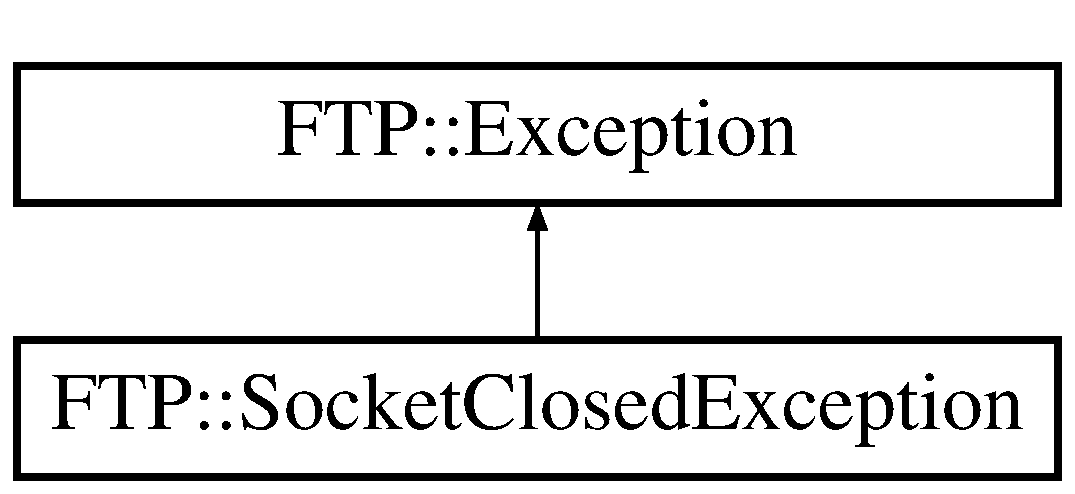
\includegraphics[height=2.000000cm]{classFTP_1_1SocketClosedException}
\end{center}
\end{figure}
\subsection*{Public Member Functions}
\begin{DoxyCompactItemize}
\item 
\hyperlink{classFTP_1_1SocketClosedException_a7cb19ab266ad0cea447bae3ded2be68a}{Socket\+Closed\+Exception} (const std\+::string \&message)
\begin{DoxyCompactList}\small\item\em \hyperlink{classFTP_1_1SocketClosedException}{Socket\+Closed\+Exception} constructor. \end{DoxyCompactList}\end{DoxyCompactItemize}


\subsection{Detailed Description}
\hyperlink{classFTP_1_1Exception}{Exception} launched when a socket close at an unexpected moment. 

\subsection{Constructor \& Destructor Documentation}
\hypertarget{classFTP_1_1SocketClosedException_a7cb19ab266ad0cea447bae3ded2be68a}{}\index{F\+T\+P\+::\+Socket\+Closed\+Exception@{F\+T\+P\+::\+Socket\+Closed\+Exception}!Socket\+Closed\+Exception@{Socket\+Closed\+Exception}}
\index{Socket\+Closed\+Exception@{Socket\+Closed\+Exception}!F\+T\+P\+::\+Socket\+Closed\+Exception@{F\+T\+P\+::\+Socket\+Closed\+Exception}}
\subsubsection[{Socket\+Closed\+Exception}]{\setlength{\rightskip}{0pt plus 5cm}F\+T\+P\+::\+Socket\+Closed\+Exception\+::\+Socket\+Closed\+Exception (
\begin{DoxyParamCaption}
\item[{const std\+::string \&}]{message}
\end{DoxyParamCaption}
)}\label{classFTP_1_1SocketClosedException_a7cb19ab266ad0cea447bae3ded2be68a}


\hyperlink{classFTP_1_1SocketClosedException}{Socket\+Closed\+Exception} constructor. 


\begin{DoxyParams}{Parameters}
{\em message} & A message to print \\
\hline
\end{DoxyParams}


The documentation for this class was generated from the following file\+:\begin{DoxyCompactItemize}
\item 
C\+:/\+Users/\+Nicolas Cachera/\+Documents/\+Programmation/\+C\+A\+R\+\_\+\+Furet\+T\+P/include/exception/Socket\+Closed\+Exception.\+h\end{DoxyCompactItemize}

\hypertarget{classFTP_1_1StorRequest}{}\section{F\+T\+P\+:\+:Stor\+Request Class Reference}
\label{classFTP_1_1StorRequest}\index{F\+T\+P\+::\+Stor\+Request@{F\+T\+P\+::\+Stor\+Request}}


Stor request.  




{\ttfamily \#include $<$Stor\+Request.\+h$>$}

Inheritance diagram for F\+T\+P\+:\+:Stor\+Request\+:\begin{figure}[H]
\begin{center}
\leavevmode
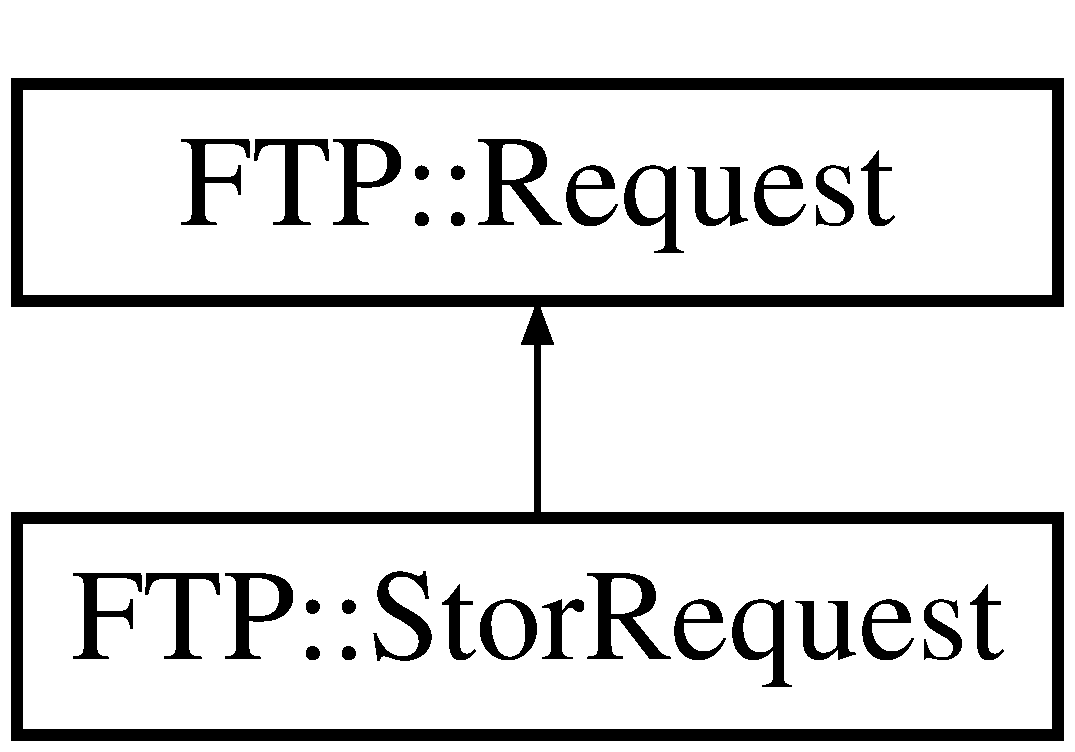
\includegraphics[height=2.000000cm]{classFTP_1_1StorRequest}
\end{center}
\end{figure}
\subsection*{Public Member Functions}
\begin{DoxyCompactItemize}
\item 
\hyperlink{classFTP_1_1StorRequest_a264af2e26c14e3523e61806e81d2025a}{Stor\+Request} (const std\+::string \&filename)
\begin{DoxyCompactList}\small\item\em \hyperlink{classFTP_1_1StorRequest}{Stor\+Request} constructor. \end{DoxyCompactList}\item 
\hypertarget{classFTP_1_1StorRequest_a21b00910bb4c7624c069054de1dfa362}{}const std\+::string \& {\bfseries get\+Filename} () const \label{classFTP_1_1StorRequest_a21b00910bb4c7624c069054de1dfa362}

\end{DoxyCompactItemize}
\subsection*{Static Public Attributes}
\begin{DoxyCompactItemize}
\item 
\hypertarget{classFTP_1_1StorRequest_af5bd83c0e967012958f8b4ee2af952b6}{}static constexpr const char $\ast$ {\bfseries Command\+Name} = \char`\"{}S\+T\+O\+R\char`\"{}\label{classFTP_1_1StorRequest_af5bd83c0e967012958f8b4ee2af952b6}

\end{DoxyCompactItemize}


\subsection{Detailed Description}
Stor request. 

Command sent by the client to upload a file on the server. 

\subsection{Constructor \& Destructor Documentation}
\hypertarget{classFTP_1_1StorRequest_a264af2e26c14e3523e61806e81d2025a}{}\index{F\+T\+P\+::\+Stor\+Request@{F\+T\+P\+::\+Stor\+Request}!Stor\+Request@{Stor\+Request}}
\index{Stor\+Request@{Stor\+Request}!F\+T\+P\+::\+Stor\+Request@{F\+T\+P\+::\+Stor\+Request}}
\subsubsection[{Stor\+Request}]{\setlength{\rightskip}{0pt plus 5cm}F\+T\+P\+::\+Stor\+Request\+::\+Stor\+Request (
\begin{DoxyParamCaption}
\item[{const std\+::string \&}]{filename}
\end{DoxyParamCaption}
)}\label{classFTP_1_1StorRequest_a264af2e26c14e3523e61806e81d2025a}


\hyperlink{classFTP_1_1StorRequest}{Stor\+Request} constructor. 


\begin{DoxyParams}{Parameters}
{\em filename} & the file to upload on the server \\
\hline
\end{DoxyParams}


The documentation for this class was generated from the following file\+:\begin{DoxyCompactItemize}
\item 
C\+:/\+Users/\+Nicolas Cachera/\+Documents/\+Programmation/\+C\+A\+R\+\_\+\+Furet\+T\+P/include/core/message/request/Stor\+Request.\+h\end{DoxyCompactItemize}

\hypertarget{classFTP_1_1SystemException}{}\section{F\+T\+P\+:\+:System\+Exception Class Reference}
\label{classFTP_1_1SystemException}\index{F\+T\+P\+::\+System\+Exception@{F\+T\+P\+::\+System\+Exception}}


\hyperlink{classFTP_1_1Exception}{Exception} for Operating system error.  




{\ttfamily \#include $<$System\+Exception.\+h$>$}

Inheritance diagram for F\+T\+P\+:\+:System\+Exception\+:\begin{figure}[H]
\begin{center}
\leavevmode
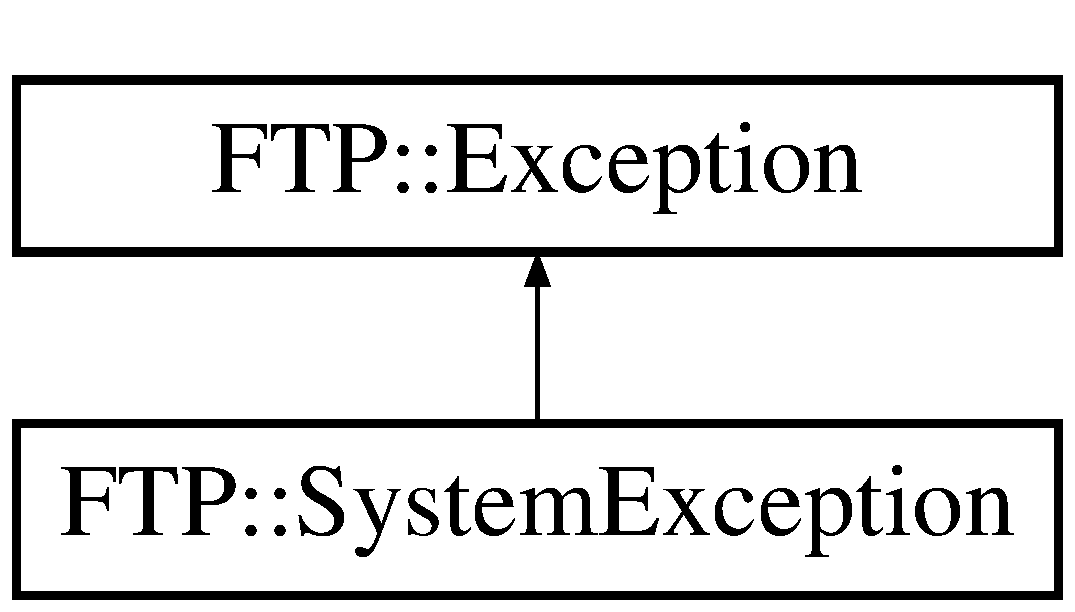
\includegraphics[height=2.000000cm]{classFTP_1_1SystemException}
\end{center}
\end{figure}
\subsection*{Public Member Functions}
\begin{DoxyCompactItemize}
\item 
\hyperlink{classFTP_1_1SystemException_a155bdb10f7e02738979d00e0510554fb}{System\+Exception} (const std\+::string \&message, int error)
\begin{DoxyCompactList}\small\item\em \hyperlink{classFTP_1_1SystemException}{System\+Exception} constructor. \end{DoxyCompactList}\end{DoxyCompactItemize}


\subsection{Detailed Description}
\hyperlink{classFTP_1_1Exception}{Exception} for Operating system error. 

\subsection{Constructor \& Destructor Documentation}
\hypertarget{classFTP_1_1SystemException_a155bdb10f7e02738979d00e0510554fb}{}\index{F\+T\+P\+::\+System\+Exception@{F\+T\+P\+::\+System\+Exception}!System\+Exception@{System\+Exception}}
\index{System\+Exception@{System\+Exception}!F\+T\+P\+::\+System\+Exception@{F\+T\+P\+::\+System\+Exception}}
\subsubsection[{System\+Exception}]{\setlength{\rightskip}{0pt plus 5cm}F\+T\+P\+::\+System\+Exception\+::\+System\+Exception (
\begin{DoxyParamCaption}
\item[{const std\+::string \&}]{message, }
\item[{int}]{error}
\end{DoxyParamCaption}
)}\label{classFTP_1_1SystemException_a155bdb10f7e02738979d00e0510554fb}


\hyperlink{classFTP_1_1SystemException}{System\+Exception} constructor. 


\begin{DoxyParams}{Parameters}
{\em message} & A message to print \\
\hline
{\em error} & The system error\textquotesingle{}s number \\
\hline
\end{DoxyParams}


The documentation for this class was generated from the following file\+:\begin{DoxyCompactItemize}
\item 
C\+:/\+Users/\+Nicolas Cachera/\+Documents/\+Programmation/\+C\+A\+R\+\_\+\+Furet\+T\+P/include/exception/System\+Exception.\+h\end{DoxyCompactItemize}

\hypertarget{classFTP_1_1SystRequest}{}\section{F\+T\+P\+:\+:Syst\+Request Class Reference}
\label{classFTP_1_1SystRequest}\index{F\+T\+P\+::\+Syst\+Request@{F\+T\+P\+::\+Syst\+Request}}


Syst request.  




{\ttfamily \#include $<$Syst\+Request.\+h$>$}

Inheritance diagram for F\+T\+P\+:\+:Syst\+Request\+:\begin{figure}[H]
\begin{center}
\leavevmode
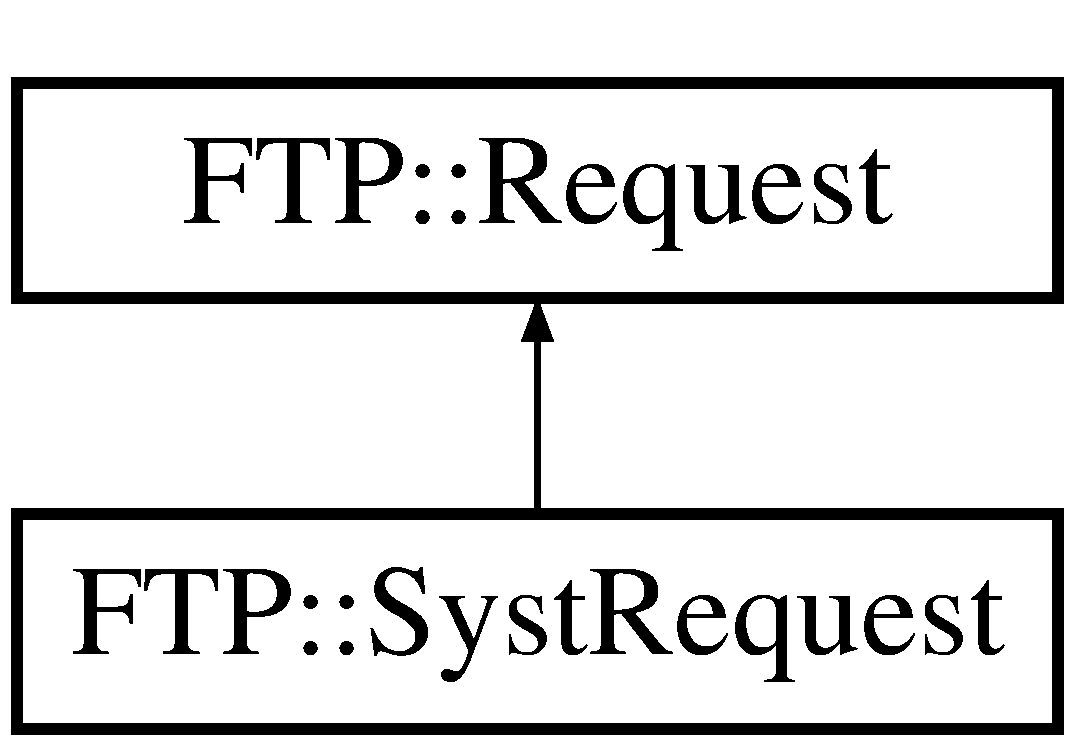
\includegraphics[height=2.000000cm]{classFTP_1_1SystRequest}
\end{center}
\end{figure}
\subsection*{Public Member Functions}
\begin{DoxyCompactItemize}
\item 
\hypertarget{classFTP_1_1SystRequest_aefe3807c83831af30762ec46f83743af}{}\hyperlink{classFTP_1_1SystRequest_aefe3807c83831af30762ec46f83743af}{Syst\+Request} ()\label{classFTP_1_1SystRequest_aefe3807c83831af30762ec46f83743af}

\begin{DoxyCompactList}\small\item\em \hyperlink{classFTP_1_1SystRequest}{Syst\+Request} constructor. \end{DoxyCompactList}\end{DoxyCompactItemize}
\subsection*{Static Public Attributes}
\begin{DoxyCompactItemize}
\item 
\hypertarget{classFTP_1_1SystRequest_a8342518a6ae8cc1f7de4aef78cbc345e}{}static constexpr const char $\ast$ {\bfseries Command\+Name} = \char`\"{}S\+Y\+S\+T\char`\"{}\label{classFTP_1_1SystRequest_a8342518a6ae8cc1f7de4aef78cbc345e}

\end{DoxyCompactItemize}


\subsection{Detailed Description}
Syst request. 

Asks the server\textquotesingle{}s system. 

The documentation for this class was generated from the following file\+:\begin{DoxyCompactItemize}
\item 
C\+:/\+Users/\+Nicolas Cachera/\+Documents/\+Programmation/\+C\+A\+R\+\_\+\+Furet\+T\+P/include/core/message/request/Syst\+Request.\+h\end{DoxyCompactItemize}

\hypertarget{classFTP_1_1Thread}{}\section{F\+T\+P\+:\+:Thread$<$ T $>$ Class Template Reference}
\label{classFTP_1_1Thread}\index{F\+T\+P\+::\+Thread$<$ T $>$@{F\+T\+P\+::\+Thread$<$ T $>$}}
\subsection*{Public Member Functions}
\begin{DoxyCompactItemize}
\item 
\hypertarget{classFTP_1_1Thread_a05e8388a05898b5e12ad102686bc370f}{}\hyperlink{classFTP_1_1Thread_a05e8388a05898b5e12ad102686bc370f}{Thread} (T $\ast$target)\label{classFTP_1_1Thread_a05e8388a05898b5e12ad102686bc370f}

\begin{DoxyCompactList}\small\item\em Create new thread with class instance target of type T. \end{DoxyCompactList}\item 
\hypertarget{classFTP_1_1Thread_adb6eb9864223b888a2d20e7349e0d57a}{}void \hyperlink{classFTP_1_1Thread_adb6eb9864223b888a2d20e7349e0d57a}{run} ()\label{classFTP_1_1Thread_adb6eb9864223b888a2d20e7349e0d57a}

\begin{DoxyCompactList}\small\item\em Launch thread. \end{DoxyCompactList}\end{DoxyCompactItemize}


The documentation for this class was generated from the following file\+:\begin{DoxyCompactItemize}
\item 
C\+:/\+Users/\+Nicolas Cachera/\+Documents/\+Programmation/\+C\+A\+R\+\_\+\+Furet\+T\+P/include/system/Thread.\+h\end{DoxyCompactItemize}

\hypertarget{classFTP_1_1Thread_3_01T_01_4}{}\section{F\+T\+P\+:\+:Thread$<$ T $>$ Class Reference}
\label{classFTP_1_1Thread_3_01T_01_4}\index{F\+T\+P\+::\+Thread$<$ T $>$@{F\+T\+P\+::\+Thread$<$ T $>$}}


\hyperlink{classFTP_1_1Thread}{Thread} managment class.  




{\ttfamily \#include $<$Thread.\+h$>$}



\subsection{Detailed Description}
\hyperlink{classFTP_1_1Thread}{Thread} managment class. 

Enscapsulate P\+O\+S\+I\+X thread (pthread). Template parameter is the class to launch in a thread. this one need to implement method void run() 

The documentation for this class was generated from the following file\+:\begin{DoxyCompactItemize}
\item 
C\+:/\+Users/\+Nicolas Cachera/\+Documents/\+Programmation/\+C\+A\+R\+\_\+\+Furet\+T\+P/include/system/Thread.\+h\end{DoxyCompactItemize}

\hypertarget{classFTP_1_1TypeRequest}{}\section{F\+T\+P\+:\+:Type\+Request Class Reference}
\label{classFTP_1_1TypeRequest}\index{F\+T\+P\+::\+Type\+Request@{F\+T\+P\+::\+Type\+Request}}


Type request.  




{\ttfamily \#include $<$Type\+Request.\+h$>$}

Inheritance diagram for F\+T\+P\+:\+:Type\+Request\+:\begin{figure}[H]
\begin{center}
\leavevmode
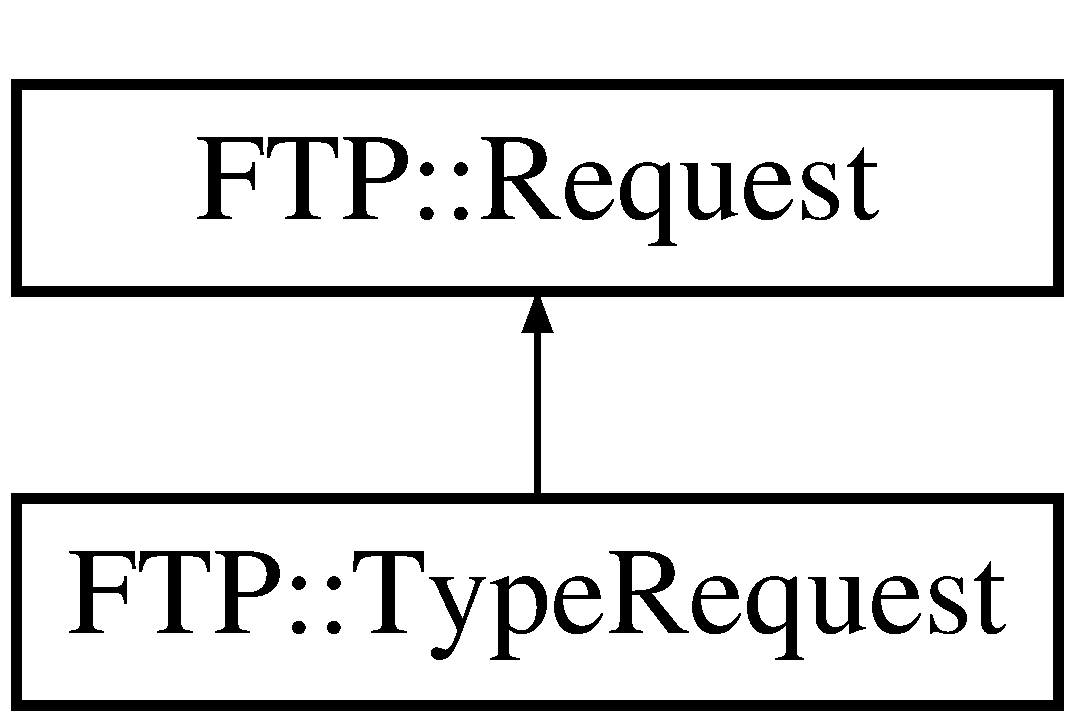
\includegraphics[height=2.000000cm]{classFTP_1_1TypeRequest}
\end{center}
\end{figure}
\subsection*{Public Types}
\begin{DoxyCompactItemize}
\item 
\hypertarget{classFTP_1_1TypeRequest_a504950a6fadf9efc043b6819170fca40}{}enum \hyperlink{classFTP_1_1TypeRequest_a504950a6fadf9efc043b6819170fca40}{Type} \{ {\bfseries Ascii}, 
{\bfseries Ebcdic}, 
{\bfseries Image}, 
{\bfseries Local}
 \}\label{classFTP_1_1TypeRequest_a504950a6fadf9efc043b6819170fca40}

\begin{DoxyCompactList}\small\item\em File type enumeration. \end{DoxyCompactList}\end{DoxyCompactItemize}
\subsection*{Public Member Functions}
\begin{DoxyCompactItemize}
\item 
\hyperlink{classFTP_1_1TypeRequest_a9583c30f4e96a6a76afe3c8864c7ad32}{Type\+Request} (\hyperlink{classFTP_1_1TypeRequest_a504950a6fadf9efc043b6819170fca40}{Type} type)
\begin{DoxyCompactList}\small\item\em \hyperlink{classFTP_1_1TypeRequest}{Type\+Request} constructor. \end{DoxyCompactList}\item 
\hypertarget{classFTP_1_1TypeRequest_a35f4fa506d33c326f6ee69435491f70f}{}\hyperlink{classFTP_1_1TypeRequest_a504950a6fadf9efc043b6819170fca40}{Type} {\bfseries get\+Type} () const \label{classFTP_1_1TypeRequest_a35f4fa506d33c326f6ee69435491f70f}

\end{DoxyCompactItemize}
\subsection*{Static Public Attributes}
\begin{DoxyCompactItemize}
\item 
\hypertarget{classFTP_1_1TypeRequest_ac9e0e4d01ceae1d3e37c8935728b39e5}{}static constexpr const char $\ast$ {\bfseries Command\+Name} = \char`\"{}T\+Y\+P\+E\char`\"{}\label{classFTP_1_1TypeRequest_ac9e0e4d01ceae1d3e37c8935728b39e5}

\end{DoxyCompactItemize}


\subsection{Detailed Description}
Type request. 

Set the type of file to be transferred 

\subsection{Constructor \& Destructor Documentation}
\hypertarget{classFTP_1_1TypeRequest_a9583c30f4e96a6a76afe3c8864c7ad32}{}\index{F\+T\+P\+::\+Type\+Request@{F\+T\+P\+::\+Type\+Request}!Type\+Request@{Type\+Request}}
\index{Type\+Request@{Type\+Request}!F\+T\+P\+::\+Type\+Request@{F\+T\+P\+::\+Type\+Request}}
\subsubsection[{Type\+Request}]{\setlength{\rightskip}{0pt plus 5cm}F\+T\+P\+::\+Type\+Request\+::\+Type\+Request (
\begin{DoxyParamCaption}
\item[{{\bf Type}}]{type}
\end{DoxyParamCaption}
)}\label{classFTP_1_1TypeRequest_a9583c30f4e96a6a76afe3c8864c7ad32}


\hyperlink{classFTP_1_1TypeRequest}{Type\+Request} constructor. 


\begin{DoxyParams}{Parameters}
{\em type} & File type to set \\
\hline
\end{DoxyParams}


The documentation for this class was generated from the following file\+:\begin{DoxyCompactItemize}
\item 
C\+:/\+Users/\+Nicolas Cachera/\+Documents/\+Programmation/\+C\+A\+R\+\_\+\+Furet\+T\+P/include/core/message/request/Type\+Request.\+h\end{DoxyCompactItemize}

\hypertarget{classFTP_1_1UnrecognizedMessageException}{}\section{F\+T\+P\+:\+:Unrecognized\+Message\+Exception Class Reference}
\label{classFTP_1_1UnrecognizedMessageException}\index{F\+T\+P\+::\+Unrecognized\+Message\+Exception@{F\+T\+P\+::\+Unrecognized\+Message\+Exception}}


\hyperlink{classFTP_1_1Exception}{Exception} launched when a message send by user isn\textquotesingle{}t recognized.  




{\ttfamily \#include $<$Unrecognized\+Message\+Exception.\+h$>$}

Inheritance diagram for F\+T\+P\+:\+:Unrecognized\+Message\+Exception\+:\begin{figure}[H]
\begin{center}
\leavevmode
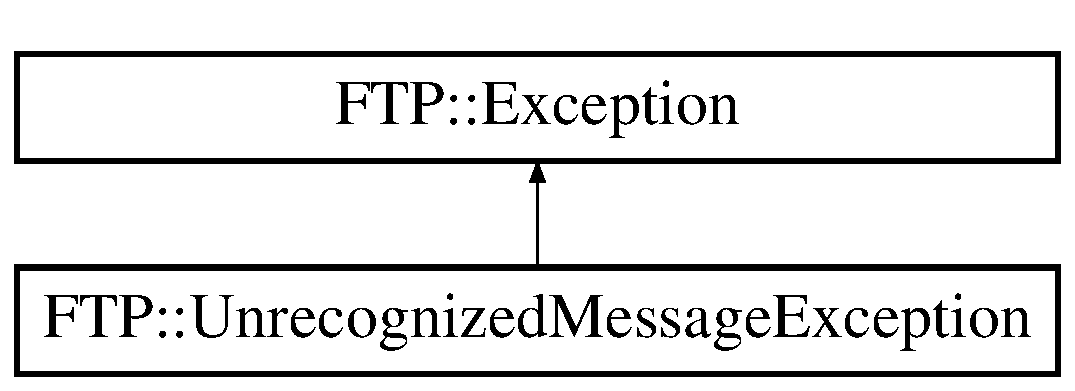
\includegraphics[height=2.000000cm]{classFTP_1_1UnrecognizedMessageException}
\end{center}
\end{figure}
\subsection*{Public Member Functions}
\begin{DoxyCompactItemize}
\item 
\hyperlink{classFTP_1_1UnrecognizedMessageException_ab4fc5bbfce2fd43536fd17ea6fc3aa4a}{Unrecognized\+Message\+Exception} (const std\+::string \&command, const std\+::string \&reason=\char`\"{}\char`\"{})
\begin{DoxyCompactList}\small\item\em \hyperlink{classFTP_1_1UnrecognizedMessageException}{Unrecognized\+Message\+Exception} constructor. \end{DoxyCompactList}\end{DoxyCompactItemize}


\subsection{Detailed Description}
\hyperlink{classFTP_1_1Exception}{Exception} launched when a message send by user isn\textquotesingle{}t recognized. 

\subsection{Constructor \& Destructor Documentation}
\hypertarget{classFTP_1_1UnrecognizedMessageException_ab4fc5bbfce2fd43536fd17ea6fc3aa4a}{}\index{F\+T\+P\+::\+Unrecognized\+Message\+Exception@{F\+T\+P\+::\+Unrecognized\+Message\+Exception}!Unrecognized\+Message\+Exception@{Unrecognized\+Message\+Exception}}
\index{Unrecognized\+Message\+Exception@{Unrecognized\+Message\+Exception}!F\+T\+P\+::\+Unrecognized\+Message\+Exception@{F\+T\+P\+::\+Unrecognized\+Message\+Exception}}
\subsubsection[{Unrecognized\+Message\+Exception}]{\setlength{\rightskip}{0pt plus 5cm}F\+T\+P\+::\+Unrecognized\+Message\+Exception\+::\+Unrecognized\+Message\+Exception (
\begin{DoxyParamCaption}
\item[{const std\+::string \&}]{command, }
\item[{const std\+::string \&}]{reason = {\ttfamily \char`\"{}\char`\"{}}}
\end{DoxyParamCaption}
)}\label{classFTP_1_1UnrecognizedMessageException_ab4fc5bbfce2fd43536fd17ea6fc3aa4a}


\hyperlink{classFTP_1_1UnrecognizedMessageException}{Unrecognized\+Message\+Exception} constructor. 


\begin{DoxyParams}{Parameters}
{\em command} & The command send by user \\
\hline
{\em reason} & The reason of unrecognition \\
\hline
\end{DoxyParams}


The documentation for this class was generated from the following file\+:\begin{DoxyCompactItemize}
\item 
C\+:/\+Users/\+Nicolas Cachera/\+Documents/\+Programmation/\+C\+A\+R\+\_\+\+Furet\+T\+P/include/exception/Unrecognized\+Message\+Exception.\+h\end{DoxyCompactItemize}

\hypertarget{structFTP_1_1User}{}\section{F\+T\+P\+:\+:User Struct Reference}
\label{structFTP_1_1User}\index{F\+T\+P\+::\+User@{F\+T\+P\+::\+User}}


Represents an user.  




{\ttfamily \#include $<$User.\+h$>$}

\subsection*{Public Member Functions}
\begin{DoxyCompactItemize}
\item 
\hypertarget{structFTP_1_1User_a1c8caf1199845f651ed9c2e259425af7}{}\hyperlink{structFTP_1_1User_a1c8caf1199845f651ed9c2e259425af7}{User} ()\label{structFTP_1_1User_a1c8caf1199845f651ed9c2e259425af7}

\begin{DoxyCompactList}\small\item\em \hyperlink{structFTP_1_1User}{User} constructor. \end{DoxyCompactList}\item 
\hyperlink{structFTP_1_1User_a9935dc6d5520daa68c4c03109723c9f2}{User} (const std\+::string \&username, const std\+::string \&password, const std\+::string \&home\+Dir, int mode)
\begin{DoxyCompactList}\small\item\em \hyperlink{structFTP_1_1User}{User} constructor. \end{DoxyCompactList}\item 
\hypertarget{structFTP_1_1User_a2de8d6c570a2b686eb751988a61fa80a}{}const std\+::string \& {\bfseries get\+Username} () const \label{structFTP_1_1User_a2de8d6c570a2b686eb751988a61fa80a}

\item 
\hypertarget{structFTP_1_1User_ae160530513b0c797a0c8c73ce3ad7349}{}const std\+::string \& {\bfseries get\+Password} () const \label{structFTP_1_1User_ae160530513b0c797a0c8c73ce3ad7349}

\item 
\hypertarget{structFTP_1_1User_a01a8869fd116660896b5fe91233719b1}{}const std\+::string \& {\bfseries get\+Home\+Dir} () const \label{structFTP_1_1User_a01a8869fd116660896b5fe91233719b1}

\item 
\hypertarget{structFTP_1_1User_abc8ec6b66316c4635d3afa42253826bc}{}int {\bfseries get\+Mode} () const \label{structFTP_1_1User_abc8ec6b66316c4635d3afa42253826bc}

\end{DoxyCompactItemize}
\subsection*{Static Public Attributes}
\begin{DoxyCompactItemize}
\item 
\hypertarget{structFTP_1_1User_ac70c77da1cd6933e556bf8f49246beb9}{}static const int {\bfseries Read\+Flag} = 0x1\label{structFTP_1_1User_ac70c77da1cd6933e556bf8f49246beb9}

\item 
\hypertarget{structFTP_1_1User_a316d807487a0e99a1019d83a5f4b2af9}{}static const int {\bfseries Write\+Flag} = 0x2\label{structFTP_1_1User_a316d807487a0e99a1019d83a5f4b2af9}

\end{DoxyCompactItemize}


\subsection{Detailed Description}
Represents an user. 

Represents an user connected to the server. 

\subsection{Constructor \& Destructor Documentation}
\hypertarget{structFTP_1_1User_a9935dc6d5520daa68c4c03109723c9f2}{}\index{F\+T\+P\+::\+User@{F\+T\+P\+::\+User}!User@{User}}
\index{User@{User}!F\+T\+P\+::\+User@{F\+T\+P\+::\+User}}
\subsubsection[{User}]{\setlength{\rightskip}{0pt plus 5cm}F\+T\+P\+::\+User\+::\+User (
\begin{DoxyParamCaption}
\item[{const std\+::string \&}]{username, }
\item[{const std\+::string \&}]{password, }
\item[{const std\+::string \&}]{home\+Dir, }
\item[{int}]{mode}
\end{DoxyParamCaption}
)}\label{structFTP_1_1User_a9935dc6d5520daa68c4c03109723c9f2}


\hyperlink{structFTP_1_1User}{User} constructor. 


\begin{DoxyParams}{Parameters}
{\em username} & \hyperlink{structFTP_1_1User}{User}\textquotesingle{}s username \\
\hline
{\em password} & \hyperlink{structFTP_1_1User}{User}\textquotesingle{}s password \\
\hline
{\em home\+Dir} & \hyperlink{structFTP_1_1User}{User}\textquotesingle{}s root directory \\
\hline
{\em user} & mode (read/write) \\
\hline
\end{DoxyParams}


The documentation for this struct was generated from the following file\+:\begin{DoxyCompactItemize}
\item 
C\+:/\+Users/\+Nicolas Cachera/\+Documents/\+Programmation/\+C\+A\+R\+\_\+\+Furet\+T\+P/include/core/User.\+h\end{DoxyCompactItemize}

\hypertarget{classFTP_1_1UserConfigurationReader}{}\section{F\+T\+P\+:\+:User\+Configuration\+Reader Class Reference}
\label{classFTP_1_1UserConfigurationReader}\index{F\+T\+P\+::\+User\+Configuration\+Reader@{F\+T\+P\+::\+User\+Configuration\+Reader}}


A class used to read a file which contains user\textquotesingle{}s account information.  




{\ttfamily \#include $<$User\+Configuration\+Reader.\+h$>$}

\subsection*{Static Public Member Functions}
\begin{DoxyCompactItemize}
\item 
static void \hyperlink{classFTP_1_1UserConfigurationReader_a2e522080a3cc4b378e82b75fc3ceb529}{process} (const std\+::string \&pathname, \hyperlink{classFTP_1_1ServerConfiguration}{Server\+Configuration} \&configuration)
\begin{DoxyCompactList}\small\item\em Read the file pathname and add the users to configuration. \end{DoxyCompactList}\end{DoxyCompactItemize}


\subsection{Detailed Description}
A class used to read a file which contains user\textquotesingle{}s account information. 

\hyperlink{classFTP_1_1UserConfigurationReader}{User\+Configuration\+Reader} is a static class. It reads a file to retrieve information about server users accounts and add them to the server configuration \hyperlink{classFTP_1_1UserList}{User\+List} 

\subsection{Member Function Documentation}
\hypertarget{classFTP_1_1UserConfigurationReader_a2e522080a3cc4b378e82b75fc3ceb529}{}\index{F\+T\+P\+::\+User\+Configuration\+Reader@{F\+T\+P\+::\+User\+Configuration\+Reader}!process@{process}}
\index{process@{process}!F\+T\+P\+::\+User\+Configuration\+Reader@{F\+T\+P\+::\+User\+Configuration\+Reader}}
\subsubsection[{process}]{\setlength{\rightskip}{0pt plus 5cm}static void F\+T\+P\+::\+User\+Configuration\+Reader\+::process (
\begin{DoxyParamCaption}
\item[{const std\+::string \&}]{pathname, }
\item[{{\bf Server\+Configuration} \&}]{configuration}
\end{DoxyParamCaption}
)\hspace{0.3cm}{\ttfamily [static]}}\label{classFTP_1_1UserConfigurationReader_a2e522080a3cc4b378e82b75fc3ceb529}


Read the file pathname and add the users to configuration. 


\begin{DoxyParams}{Parameters}
{\em pathname} & the file to read \\
\hline
{\em configuration} & the configuration where the methods will add users\\
\hline
\end{DoxyParams}
The read must contains n lines for n user. Each lines must be in the following format \+: $<$username$>$ $<$password$>$ $<$home\+\_\+dir$>$ If the file doesn\textquotesingle{}t respect this syntax, the method will throw an \hyperlink{classFTP_1_1IncorrecteFileFormatException}{Incorrecte\+File\+Format\+Exception} 

The documentation for this class was generated from the following file\+:\begin{DoxyCompactItemize}
\item 
C\+:/\+Users/\+Nicolas Cachera/\+Documents/\+Programmation/\+C\+A\+R\+\_\+\+Furet\+T\+P/include/core/User\+Configuration\+Reader.\+h\end{DoxyCompactItemize}

\hypertarget{classFTP_1_1UserList}{}\section{F\+T\+P\+:\+:User\+List Class Reference}
\label{classFTP_1_1UserList}\index{F\+T\+P\+::\+User\+List@{F\+T\+P\+::\+User\+List}}


Represents a list of users.  




{\ttfamily \#include $<$User.\+h$>$}

\subsection*{Public Member Functions}
\begin{DoxyCompactItemize}
\item 
\hypertarget{classFTP_1_1UserList_af2f3d0d0df23f6a00bea95f0be707601}{}\hyperlink{classFTP_1_1UserList_af2f3d0d0df23f6a00bea95f0be707601}{User\+List} ()\label{classFTP_1_1UserList_af2f3d0d0df23f6a00bea95f0be707601}

\begin{DoxyCompactList}\small\item\em \hyperlink{classFTP_1_1UserList}{User\+List} constructor. \end{DoxyCompactList}\item 
bool \hyperlink{classFTP_1_1UserList_a0427b71d7f5c0ed383cb6254f36d210c}{add\+User} (const \hyperlink{structFTP_1_1User}{User} \&user)
\begin{DoxyCompactList}\small\item\em Add an user to the list. \end{DoxyCompactList}\item 
const \hyperlink{structFTP_1_1User}{User} \& \hyperlink{classFTP_1_1UserList_a260d4aa185854aefa9266e762fb5a0dc}{find\+User} (const std\+::string \&username) const 
\begin{DoxyCompactList}\small\item\em Find an user with his username in the list. \end{DoxyCompactList}\item 
bool \hyperlink{classFTP_1_1UserList_a9b6441c5595dbdcdd872d4c3182da44a}{has\+User} (const std\+::string \&username) const 
\begin{DoxyCompactList}\small\item\em has\+User Says if the list contains an user with the username username \end{DoxyCompactList}\end{DoxyCompactItemize}


\subsection{Detailed Description}
Represents a list of users. 

Represents a list of users connected to the server. 

\subsection{Member Function Documentation}
\hypertarget{classFTP_1_1UserList_a0427b71d7f5c0ed383cb6254f36d210c}{}\index{F\+T\+P\+::\+User\+List@{F\+T\+P\+::\+User\+List}!add\+User@{add\+User}}
\index{add\+User@{add\+User}!F\+T\+P\+::\+User\+List@{F\+T\+P\+::\+User\+List}}
\subsubsection[{add\+User}]{\setlength{\rightskip}{0pt plus 5cm}bool F\+T\+P\+::\+User\+List\+::add\+User (
\begin{DoxyParamCaption}
\item[{const {\bf User} \&}]{user}
\end{DoxyParamCaption}
)}\label{classFTP_1_1UserList_a0427b71d7f5c0ed383cb6254f36d210c}


Add an user to the list. 


\begin{DoxyParams}{Parameters}
{\em user} & The user to add \\
\hline
\end{DoxyParams}
\begin{DoxyReturn}{Returns}
True if the user is added, false otherwise 
\end{DoxyReturn}
\hypertarget{classFTP_1_1UserList_a260d4aa185854aefa9266e762fb5a0dc}{}\index{F\+T\+P\+::\+User\+List@{F\+T\+P\+::\+User\+List}!find\+User@{find\+User}}
\index{find\+User@{find\+User}!F\+T\+P\+::\+User\+List@{F\+T\+P\+::\+User\+List}}
\subsubsection[{find\+User}]{\setlength{\rightskip}{0pt plus 5cm}const {\bf User}\& F\+T\+P\+::\+User\+List\+::find\+User (
\begin{DoxyParamCaption}
\item[{const std\+::string \&}]{username}
\end{DoxyParamCaption}
) const}\label{classFTP_1_1UserList_a260d4aa185854aefa9266e762fb5a0dc}


Find an user with his username in the list. 


\begin{DoxyParams}{Parameters}
{\em username} & the username of the user we\textquotesingle{}re searching for \\
\hline
\end{DoxyParams}
\begin{DoxyReturn}{Returns}
the user if he\textquotesingle{}s finded, throw an \hyperlink{classFTP_1_1UserNotFoundException}{User\+Not\+Found\+Exception} otherwise 
\end{DoxyReturn}
\hypertarget{classFTP_1_1UserList_a9b6441c5595dbdcdd872d4c3182da44a}{}\index{F\+T\+P\+::\+User\+List@{F\+T\+P\+::\+User\+List}!has\+User@{has\+User}}
\index{has\+User@{has\+User}!F\+T\+P\+::\+User\+List@{F\+T\+P\+::\+User\+List}}
\subsubsection[{has\+User}]{\setlength{\rightskip}{0pt plus 5cm}bool F\+T\+P\+::\+User\+List\+::has\+User (
\begin{DoxyParamCaption}
\item[{const std\+::string \&}]{username}
\end{DoxyParamCaption}
) const}\label{classFTP_1_1UserList_a9b6441c5595dbdcdd872d4c3182da44a}


has\+User Says if the list contains an user with the username username 


\begin{DoxyParams}{Parameters}
{\em username} & \\
\hline
\end{DoxyParams}
\begin{DoxyReturn}{Returns}
True if the list contains the user username, False otherwise 
\end{DoxyReturn}


The documentation for this class was generated from the following file\+:\begin{DoxyCompactItemize}
\item 
C\+:/\+Users/\+Nicolas Cachera/\+Documents/\+Programmation/\+C\+A\+R\+\_\+\+Furet\+T\+P/include/core/User.\+h\end{DoxyCompactItemize}

\input{classftp_1_1UserList}
\hypertarget{classFTP_1_1UserNotFoundException}{}\section{F\+T\+P\+:\+:User\+Not\+Found\+Exception Class Reference}
\label{classFTP_1_1UserNotFoundException}\index{F\+T\+P\+::\+User\+Not\+Found\+Exception@{F\+T\+P\+::\+User\+Not\+Found\+Exception}}


\hyperlink{classFTP_1_1Exception}{Exception} launched when a user isn\textquotesingle{}t found.  




{\ttfamily \#include $<$User\+Not\+Found\+Exception.\+h$>$}

Inheritance diagram for F\+T\+P\+:\+:User\+Not\+Found\+Exception\+:\begin{figure}[H]
\begin{center}
\leavevmode
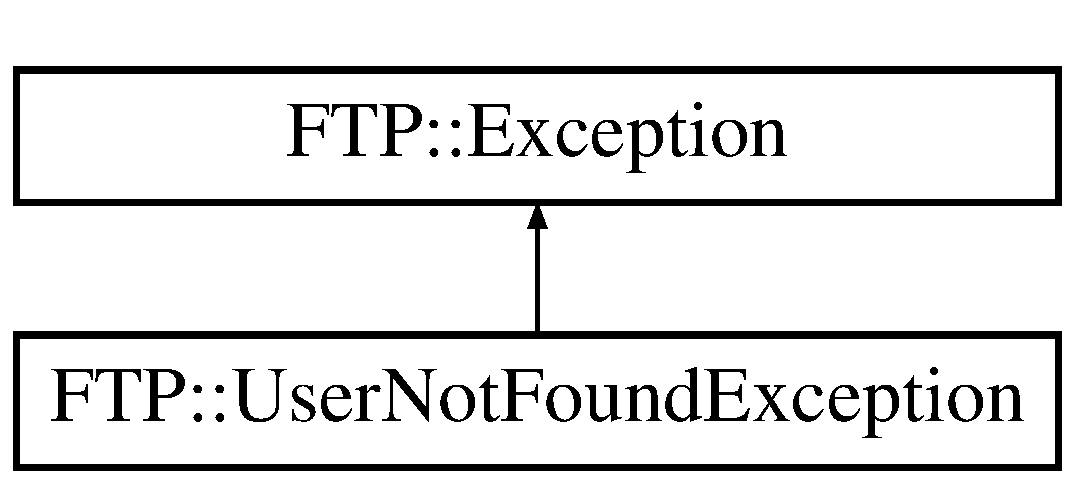
\includegraphics[height=2.000000cm]{classFTP_1_1UserNotFoundException}
\end{center}
\end{figure}
\subsection*{Public Member Functions}
\begin{DoxyCompactItemize}
\item 
\hyperlink{classFTP_1_1UserNotFoundException_af6320749bd19931a899717361fd71739}{User\+Not\+Found\+Exception} (const std\+::string \&username)
\begin{DoxyCompactList}\small\item\em \hyperlink{classFTP_1_1UserNotFoundException}{User\+Not\+Found\+Exception} constructor. \end{DoxyCompactList}\end{DoxyCompactItemize}


\subsection{Detailed Description}
\hyperlink{classFTP_1_1Exception}{Exception} launched when a user isn\textquotesingle{}t found. 

\subsection{Constructor \& Destructor Documentation}
\hypertarget{classFTP_1_1UserNotFoundException_af6320749bd19931a899717361fd71739}{}\index{F\+T\+P\+::\+User\+Not\+Found\+Exception@{F\+T\+P\+::\+User\+Not\+Found\+Exception}!User\+Not\+Found\+Exception@{User\+Not\+Found\+Exception}}
\index{User\+Not\+Found\+Exception@{User\+Not\+Found\+Exception}!F\+T\+P\+::\+User\+Not\+Found\+Exception@{F\+T\+P\+::\+User\+Not\+Found\+Exception}}
\subsubsection[{User\+Not\+Found\+Exception}]{\setlength{\rightskip}{0pt plus 5cm}F\+T\+P\+::\+User\+Not\+Found\+Exception\+::\+User\+Not\+Found\+Exception (
\begin{DoxyParamCaption}
\item[{const std\+::string \&}]{username}
\end{DoxyParamCaption}
)}\label{classFTP_1_1UserNotFoundException_af6320749bd19931a899717361fd71739}


\hyperlink{classFTP_1_1UserNotFoundException}{User\+Not\+Found\+Exception} constructor. 


\begin{DoxyParams}{Parameters}
{\em username} & The name of the user \\
\hline
\end{DoxyParams}


The documentation for this class was generated from the following file\+:\begin{DoxyCompactItemize}
\item 
C\+:/\+Users/\+Nicolas Cachera/\+Documents/\+Programmation/\+C\+A\+R\+\_\+\+Furet\+T\+P/include/exception/User\+Not\+Found\+Exception.\+h\end{DoxyCompactItemize}

\hypertarget{classFTP_1_1UserRequest}{}\section{F\+T\+P\+:\+:User\+Request Class Reference}
\label{classFTP_1_1UserRequest}\index{F\+T\+P\+::\+User\+Request@{F\+T\+P\+::\+User\+Request}}


\hyperlink{structFTP_1_1User}{User} request.  




{\ttfamily \#include $<$User\+Request.\+h$>$}

Inheritance diagram for F\+T\+P\+:\+:User\+Request\+:\begin{figure}[H]
\begin{center}
\leavevmode
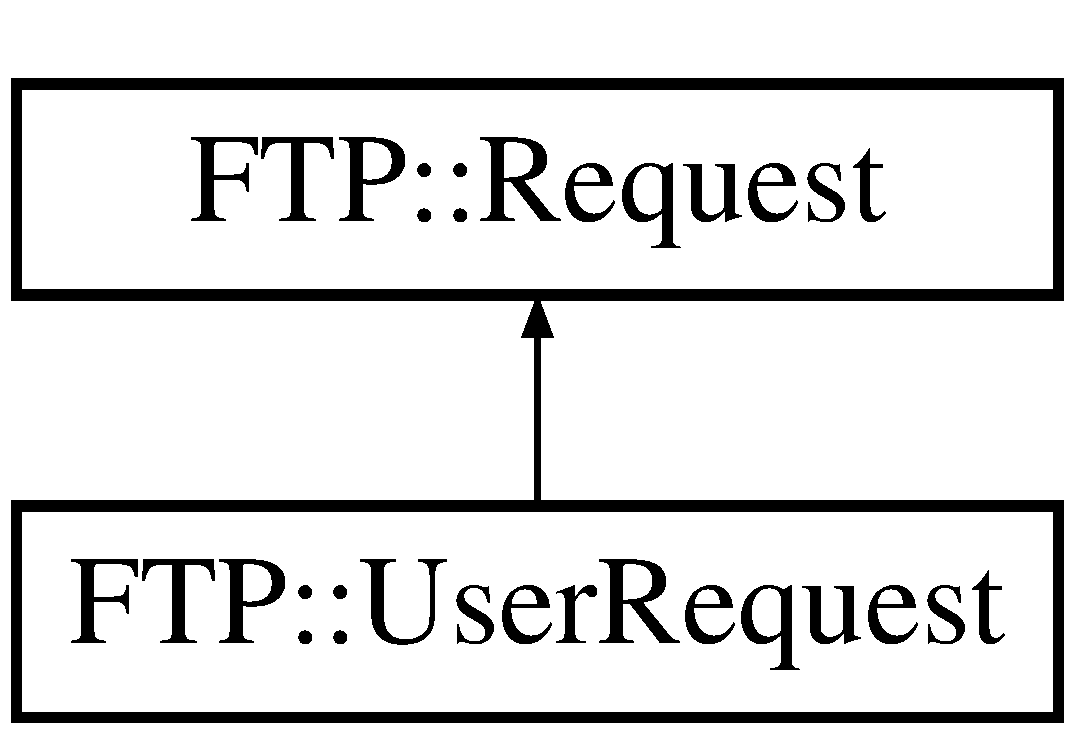
\includegraphics[height=2.000000cm]{classFTP_1_1UserRequest}
\end{center}
\end{figure}
\subsection*{Public Member Functions}
\begin{DoxyCompactItemize}
\item 
\hyperlink{classFTP_1_1UserRequest_a385e73c2e46f88f757c20748a0f52a0f}{User\+Request} (const std\+::string \&username)
\begin{DoxyCompactList}\small\item\em \hyperlink{classFTP_1_1UserRequest}{User\+Request} constructor. \end{DoxyCompactList}\item 
\hypertarget{classFTP_1_1UserRequest_a0a795f933d6b956aa1ea20e41f22f45b}{}const std\+::string \& {\bfseries get\+Username} () const \label{classFTP_1_1UserRequest_a0a795f933d6b956aa1ea20e41f22f45b}

\end{DoxyCompactItemize}
\subsection*{Static Public Attributes}
\begin{DoxyCompactItemize}
\item 
\hypertarget{classFTP_1_1UserRequest_a1d62befcdffbc41a256e92954fa0fb4c}{}static constexpr const char $\ast$ {\bfseries Command\+Name} = \char`\"{}U\+S\+E\+R\char`\"{}\label{classFTP_1_1UserRequest_a1d62befcdffbc41a256e92954fa0fb4c}

\end{DoxyCompactItemize}


\subsection{Detailed Description}
\hyperlink{structFTP_1_1User}{User} request. 

\hyperlink{classFTP_1_1Request}{Request} sent when user begins login. This command contains the username as first argument. 

\subsection{Constructor \& Destructor Documentation}
\hypertarget{classFTP_1_1UserRequest_a385e73c2e46f88f757c20748a0f52a0f}{}\index{F\+T\+P\+::\+User\+Request@{F\+T\+P\+::\+User\+Request}!User\+Request@{User\+Request}}
\index{User\+Request@{User\+Request}!F\+T\+P\+::\+User\+Request@{F\+T\+P\+::\+User\+Request}}
\subsubsection[{User\+Request}]{\setlength{\rightskip}{0pt plus 5cm}F\+T\+P\+::\+User\+Request\+::\+User\+Request (
\begin{DoxyParamCaption}
\item[{const std\+::string \&}]{username}
\end{DoxyParamCaption}
)}\label{classFTP_1_1UserRequest_a385e73c2e46f88f757c20748a0f52a0f}


\hyperlink{classFTP_1_1UserRequest}{User\+Request} constructor. 


\begin{DoxyParams}{Parameters}
{\em username} & \hyperlink{structFTP_1_1User}{User}\textquotesingle{}s username \\
\hline
\end{DoxyParams}


The documentation for this class was generated from the following file\+:\begin{DoxyCompactItemize}
\item 
C\+:/\+Users/\+Nicolas Cachera/\+Documents/\+Programmation/\+C\+A\+R\+\_\+\+Furet\+T\+P/include/core/message/request/User\+Request.\+h\end{DoxyCompactItemize}

%--- End generated contents ---

% Index
\backmatter
\newpage
\phantomsection
\clearemptydoublepage
\addcontentsline{toc}{chapter}{Index}
\printindex

\end{document}
